\section{Results}

As the complete stucture to analize was symmetrical, only a half of it was modeled with a transfinite mesh and studied, as shown bellow.

The complete thickness of the structure was defined as 20 mm.

\begin{figure}[H]
    \centering
    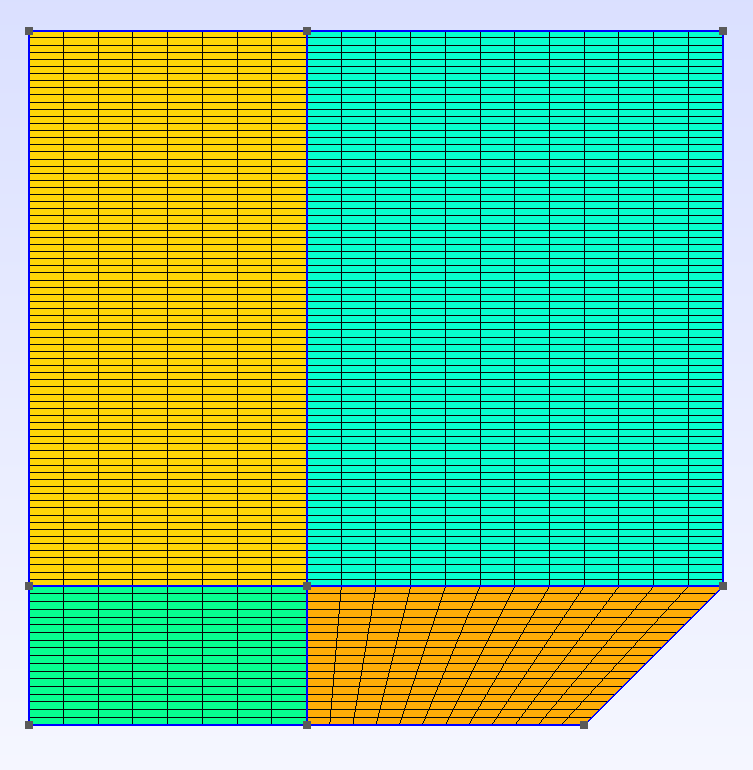
\includegraphics[width=0.5\textwidth]{img/geometria.png}
    \caption{Half structure modeled in GMSH}
    \label{fig:half_structure}
\end{figure}

\subsection{Part b)}

In this section, a stress analysis was made over 4 different mesh sizes using two refinment techniques, global and local refinment, for both element types.

For the global refinment, the characteristic size h was modified uniformly across the entire mesh, varying its value from 2 mm up to 1.25 mm. These values were determined based on the time required for the simulation to run and the capacity of the software to refine the mesh.

In the case of local refinment, the characteristic size h was modified in a specific region of the mesh, near the stress concentration area, in other words, the right border. For this to be studied, the number of elements was higher in that zone compared to the left border.

The results of refining the mesh globally and locally are shown in the following sections.

\subsubsection{Quad4 Element}

The following maps shows how the stress distribution changes with the mesh size as it is refined using Quad4 elements.

\begin{figure}[H]
  \centering
  \begin{subfigure}[b]{0.45\textwidth}
    \centering
    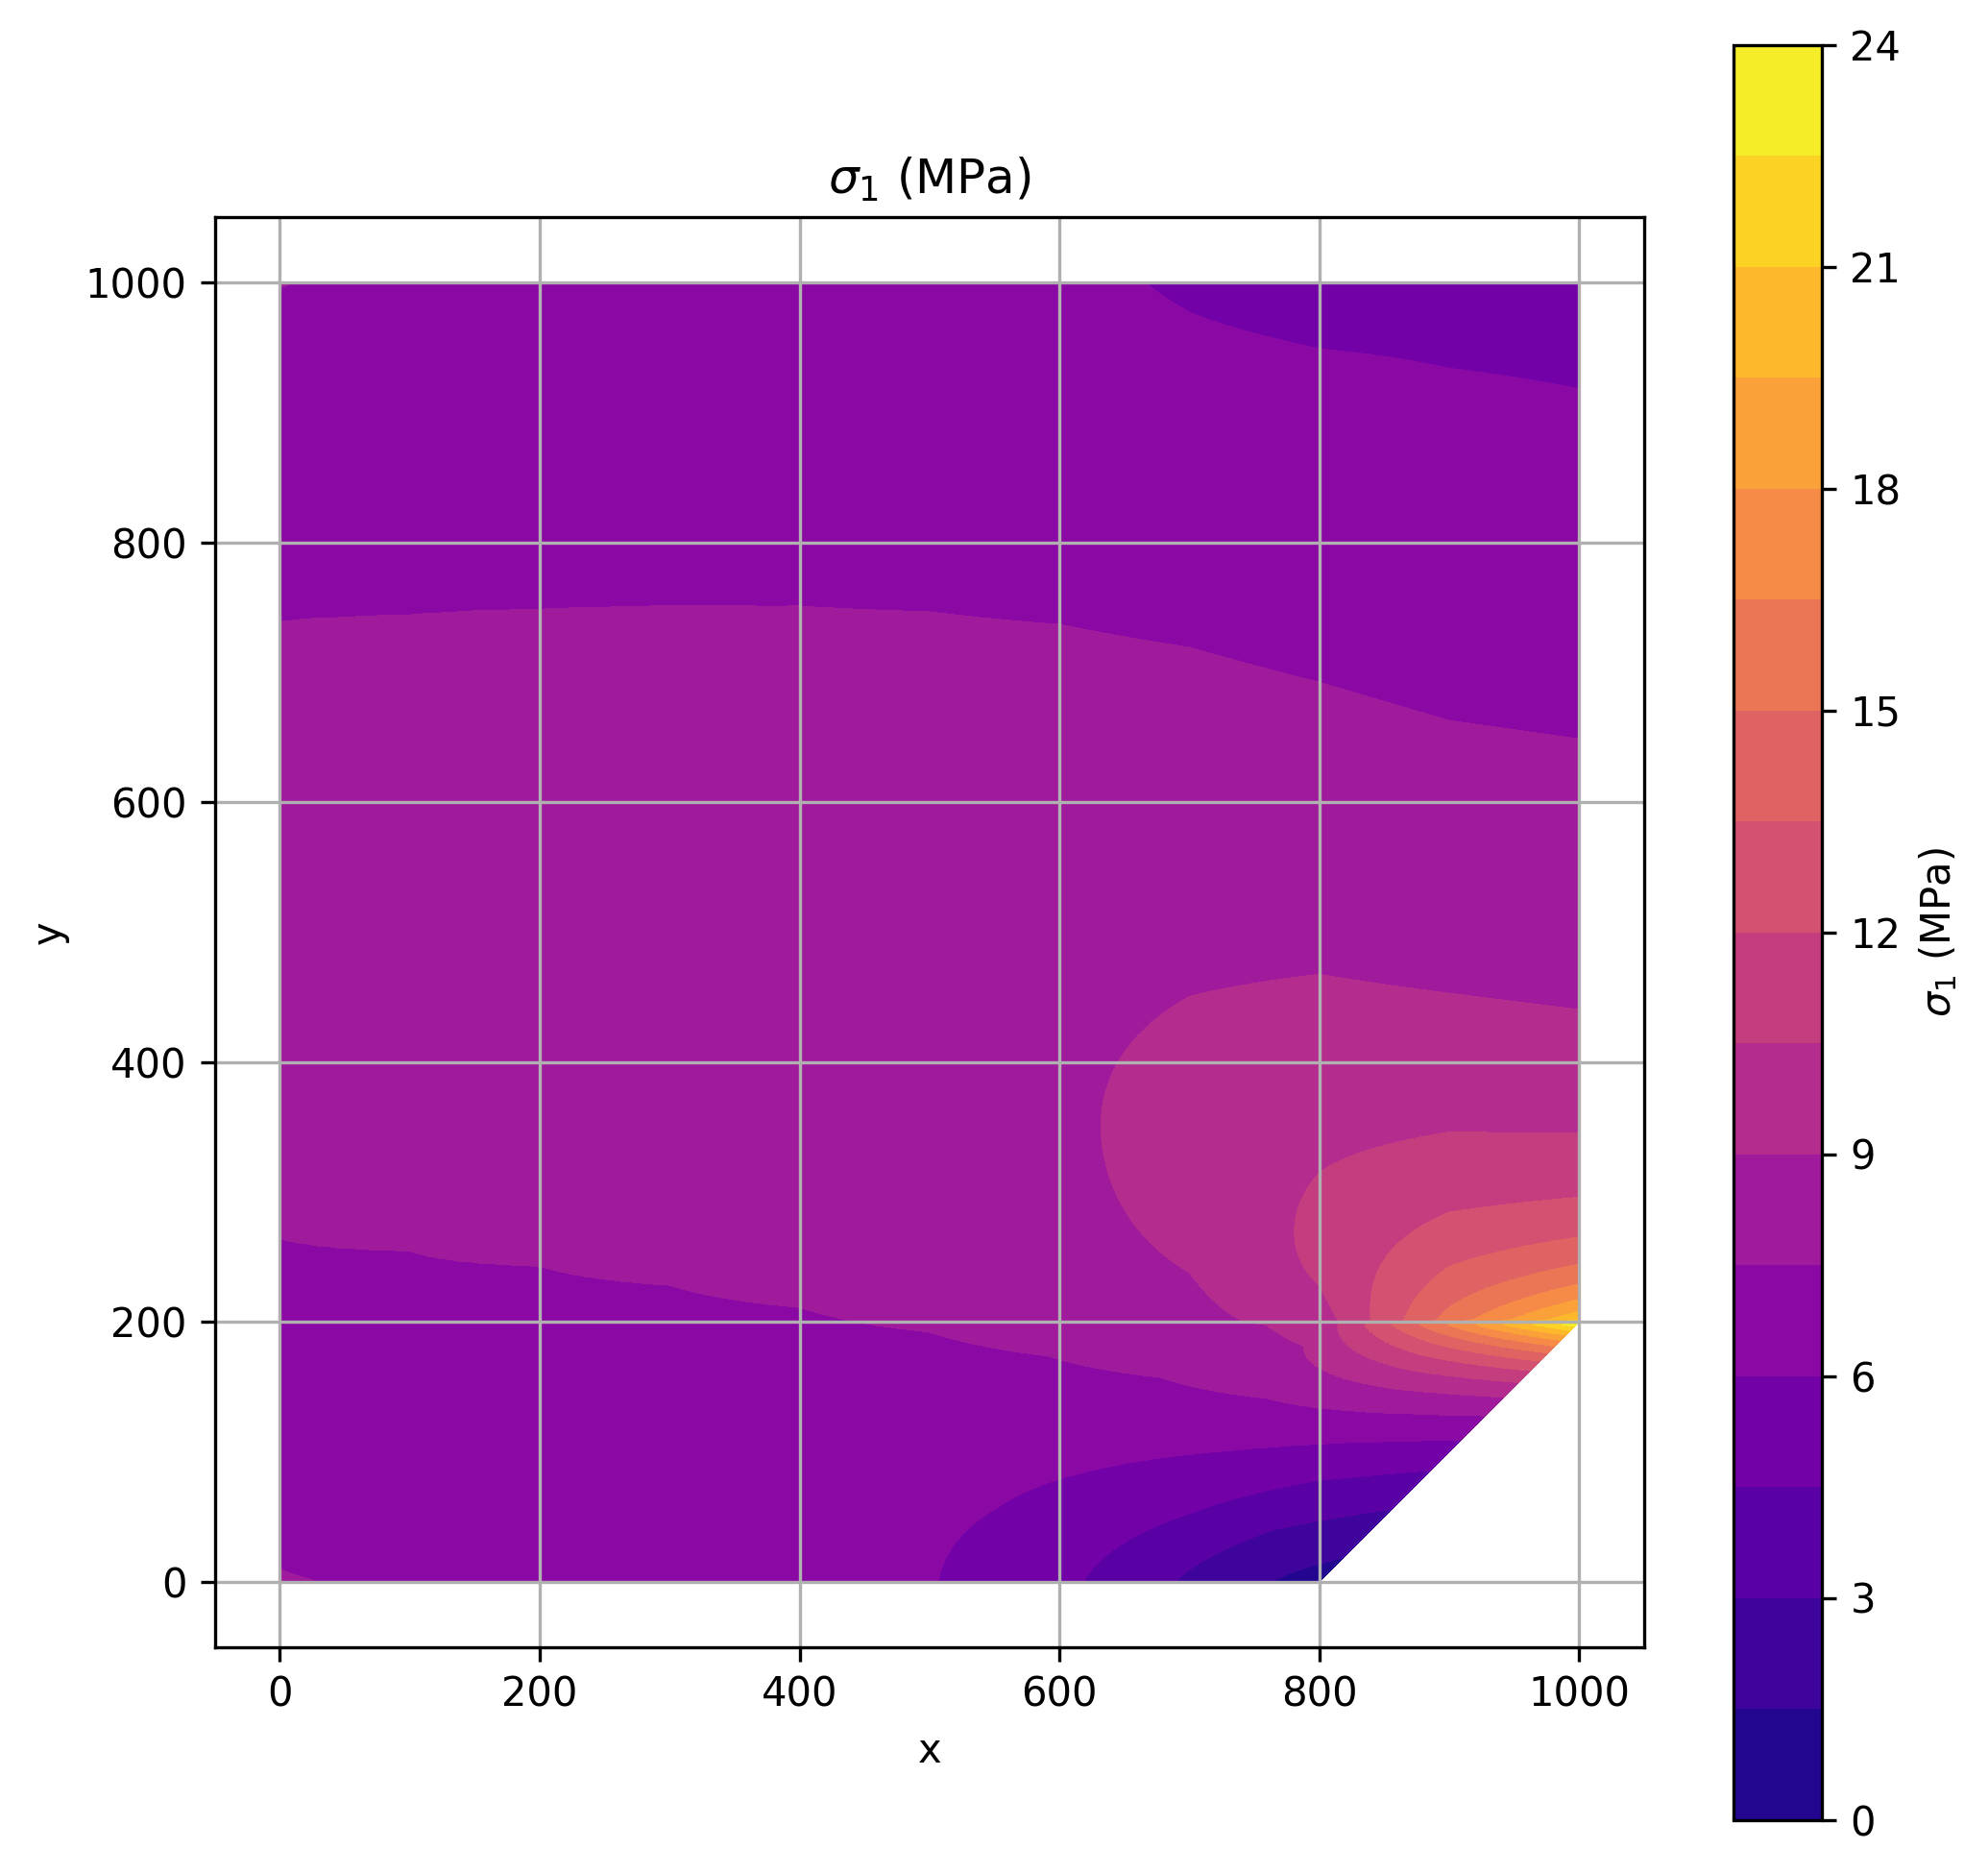
\includegraphics[width=\textwidth]{GRAFICOS/Quad4/2mm_global/resultados - sigma_1.png}
    \caption{Global mesh refinement - $h=2mm$}
    \label{fig:img1}
  \end{subfigure}
  \hfill
  \begin{subfigure}[b]{0.45\textwidth}
    \centering
    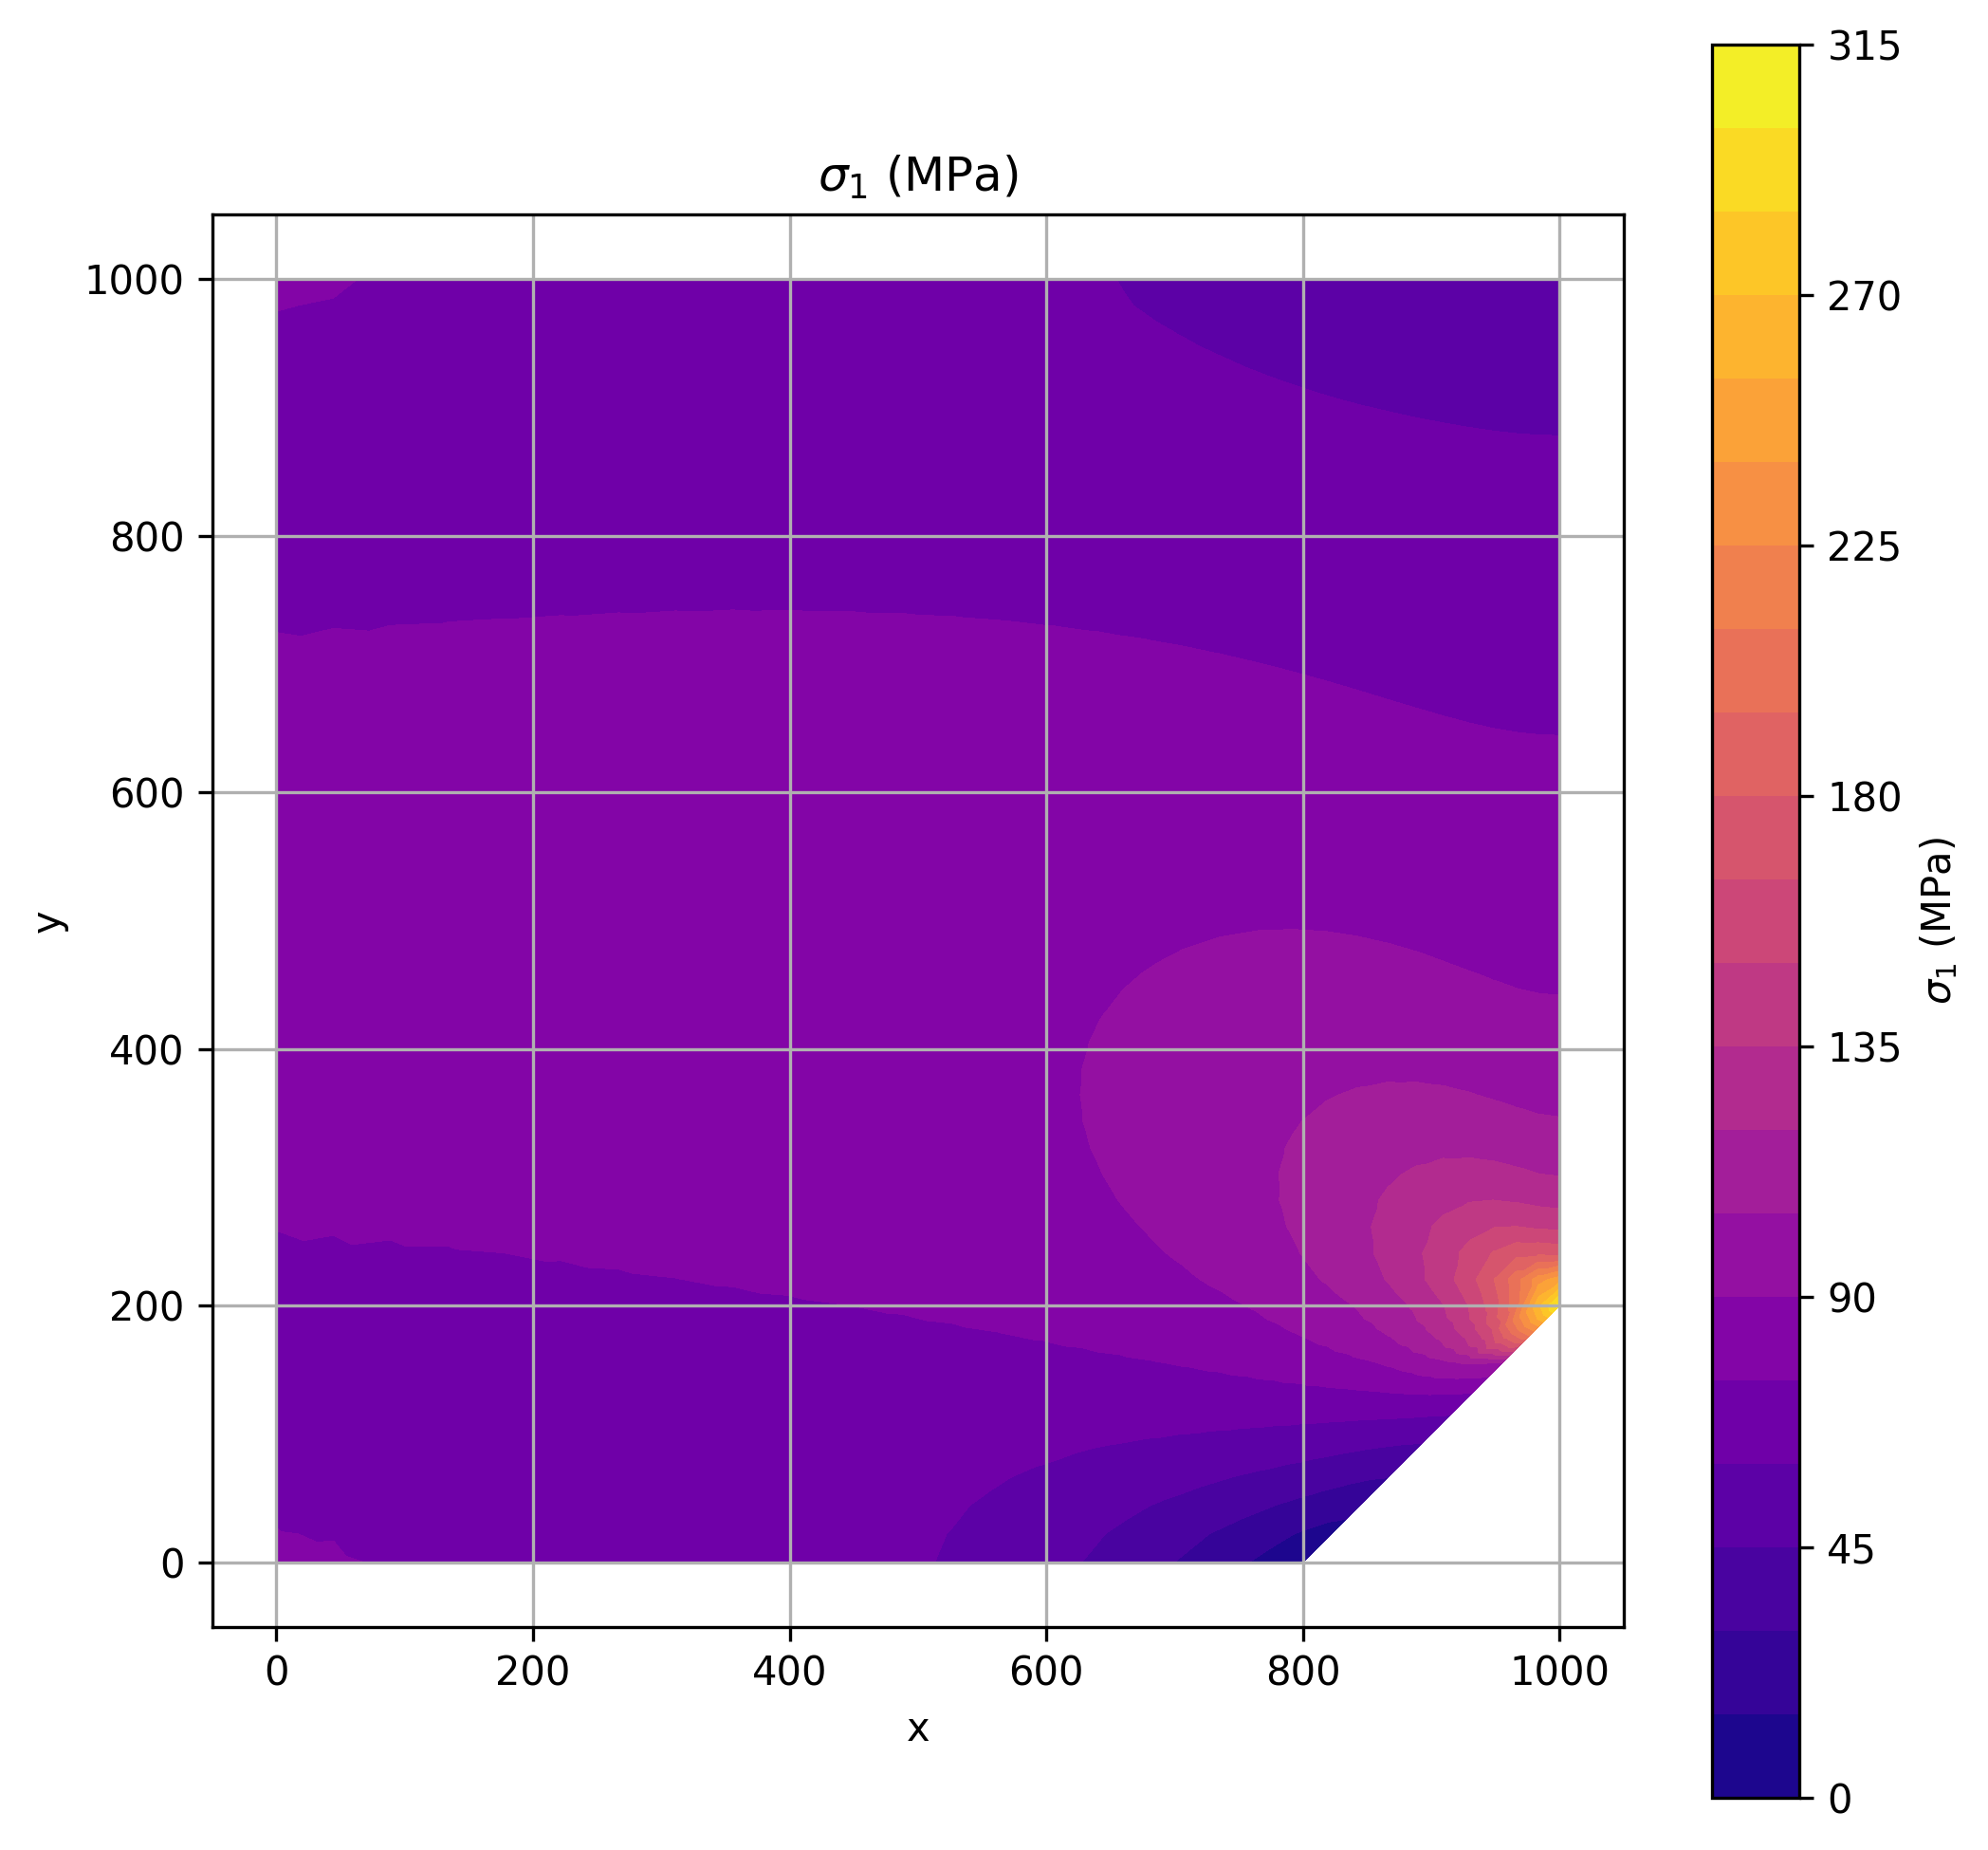
\includegraphics[width=\textwidth]{GRAFICOS/Quad4/2mm_local/resultados - sigma_1.png}
    \caption{Local mesh refinement - $h=2mm$}
    \label{fig:img2}
  \end{subfigure}
\end{figure}

\begin{figure}[H]
  \centering
  \begin{subfigure}[b]{0.45\textwidth}
    \centering
    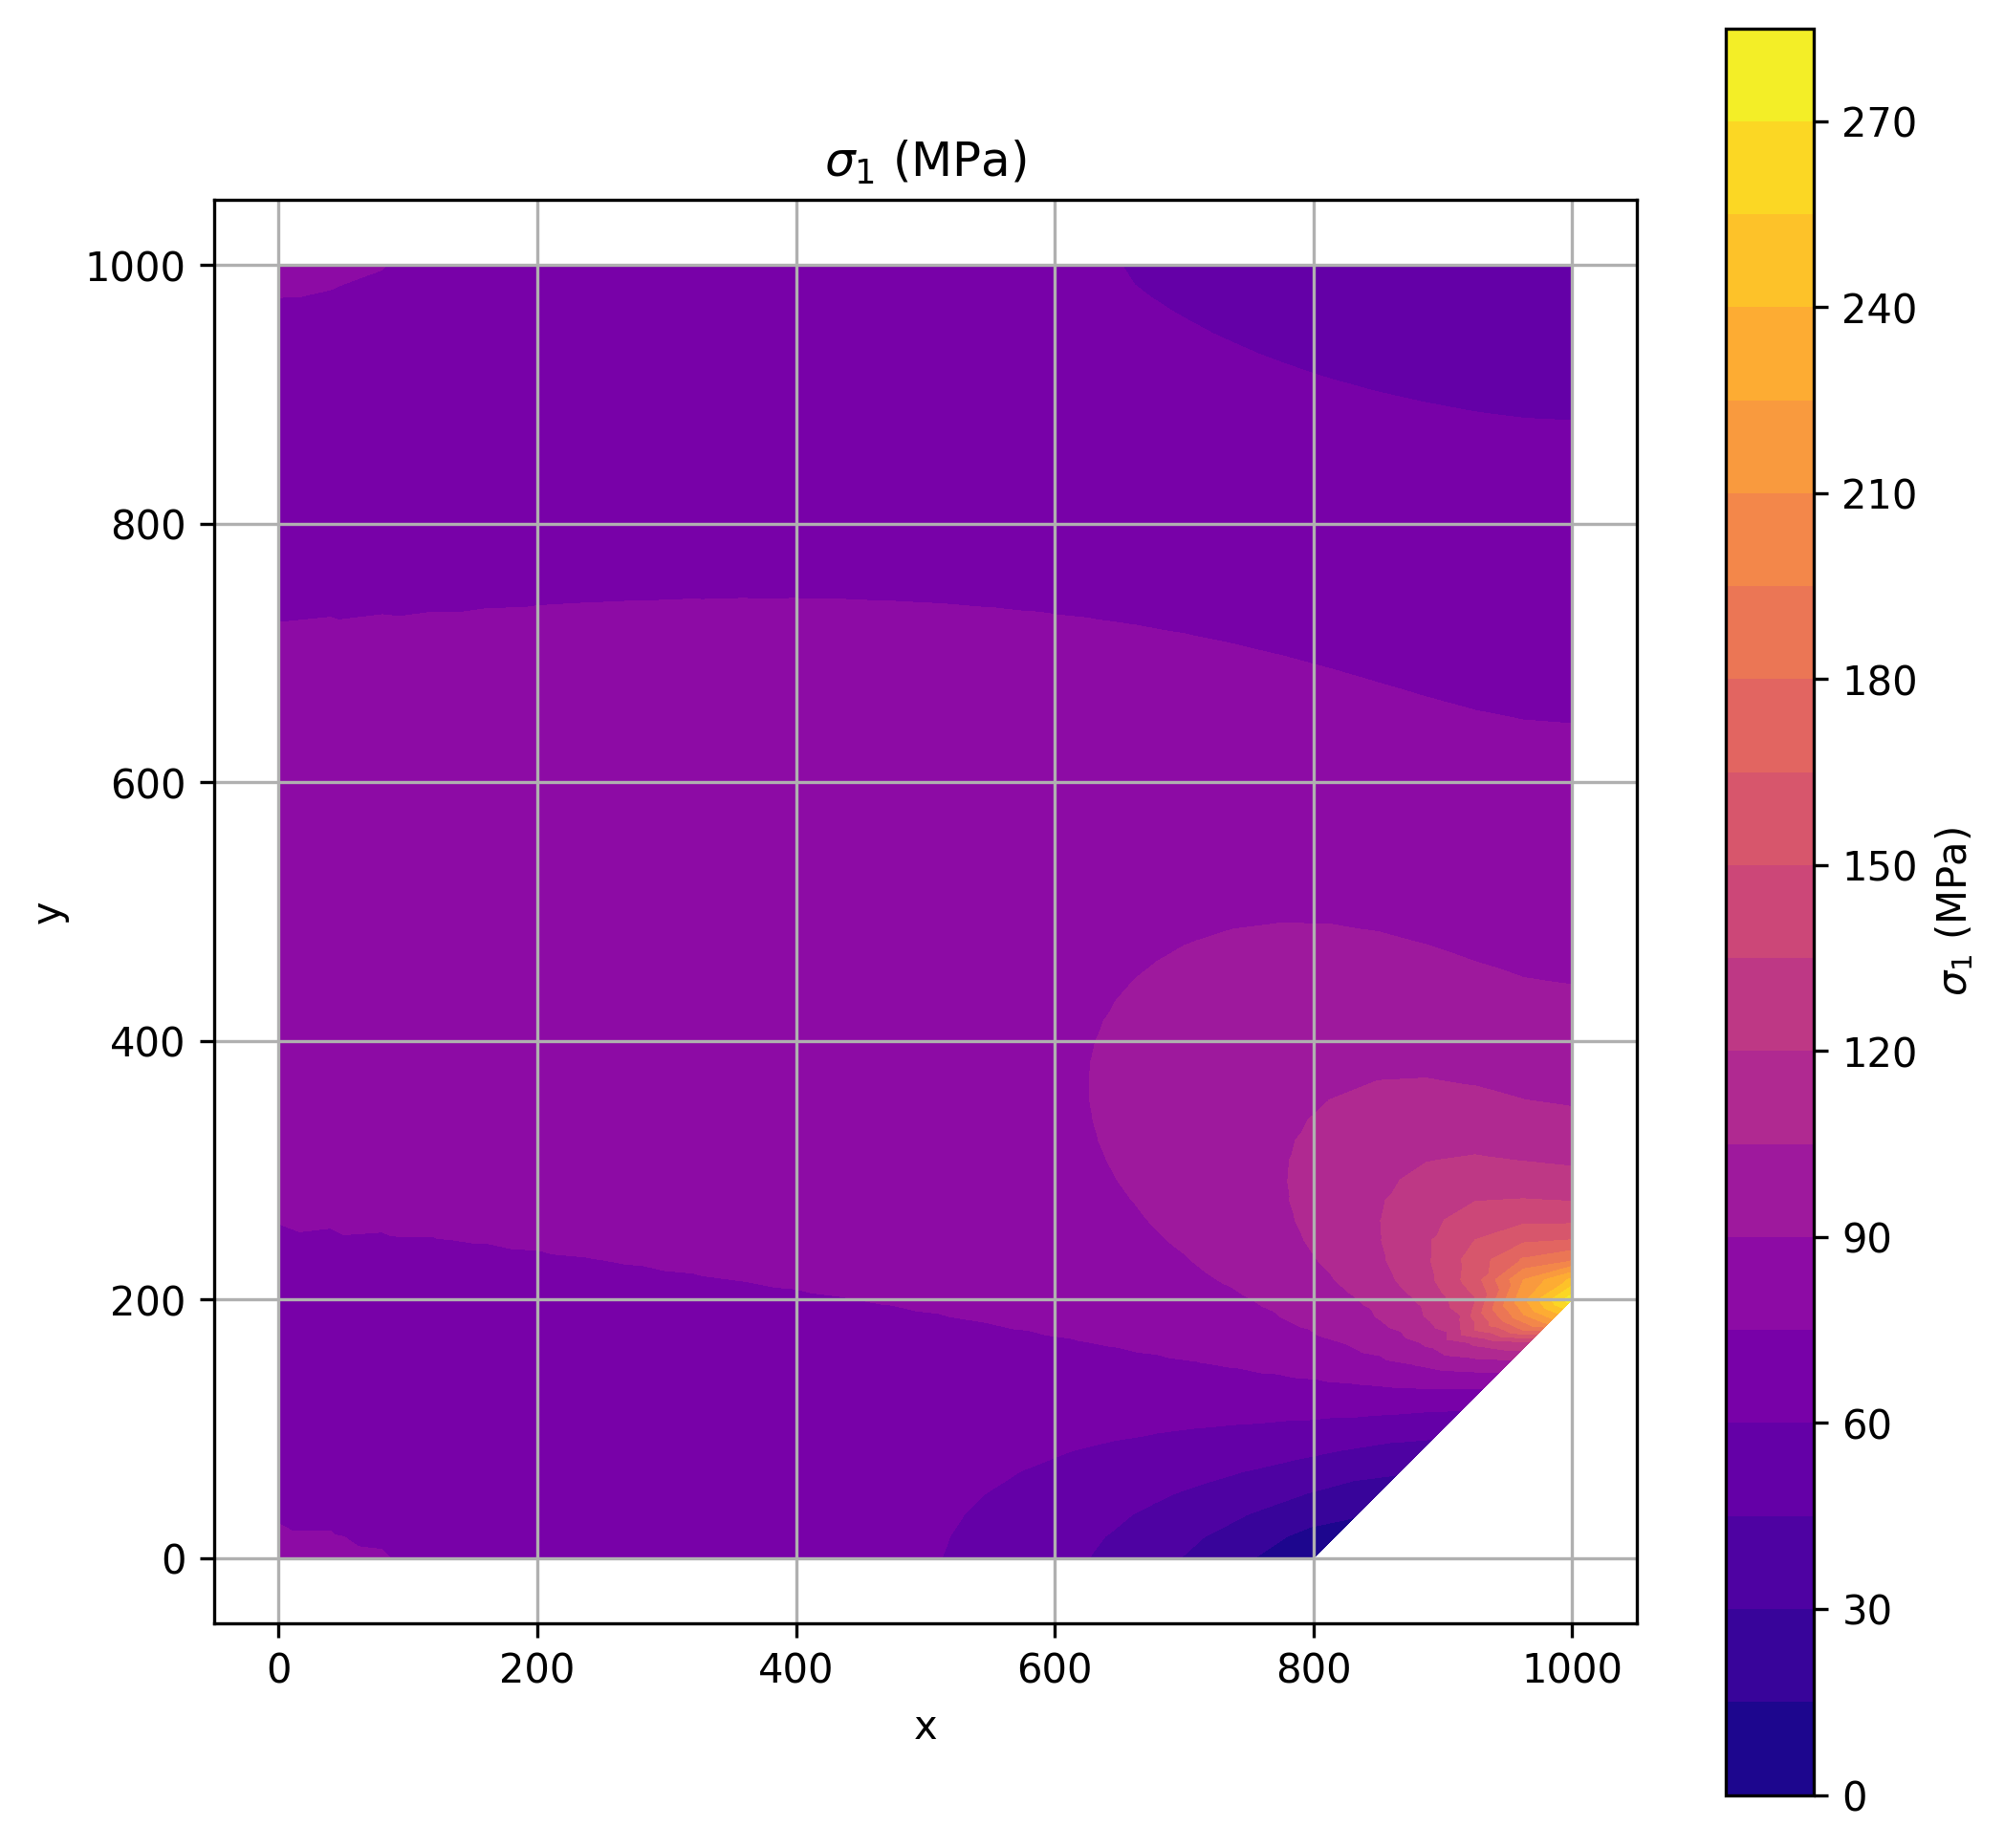
\includegraphics[width=\textwidth]{GRAFICOS/Quad4/1.75mm_global/resultados - sigma_1.png}
    \caption{Global mesh refinement - $h=1.75mm$}
    \label{fig:img11}
  \end{subfigure}
  \hfill
  \begin{subfigure}[b]{0.45\textwidth}
    \centering
    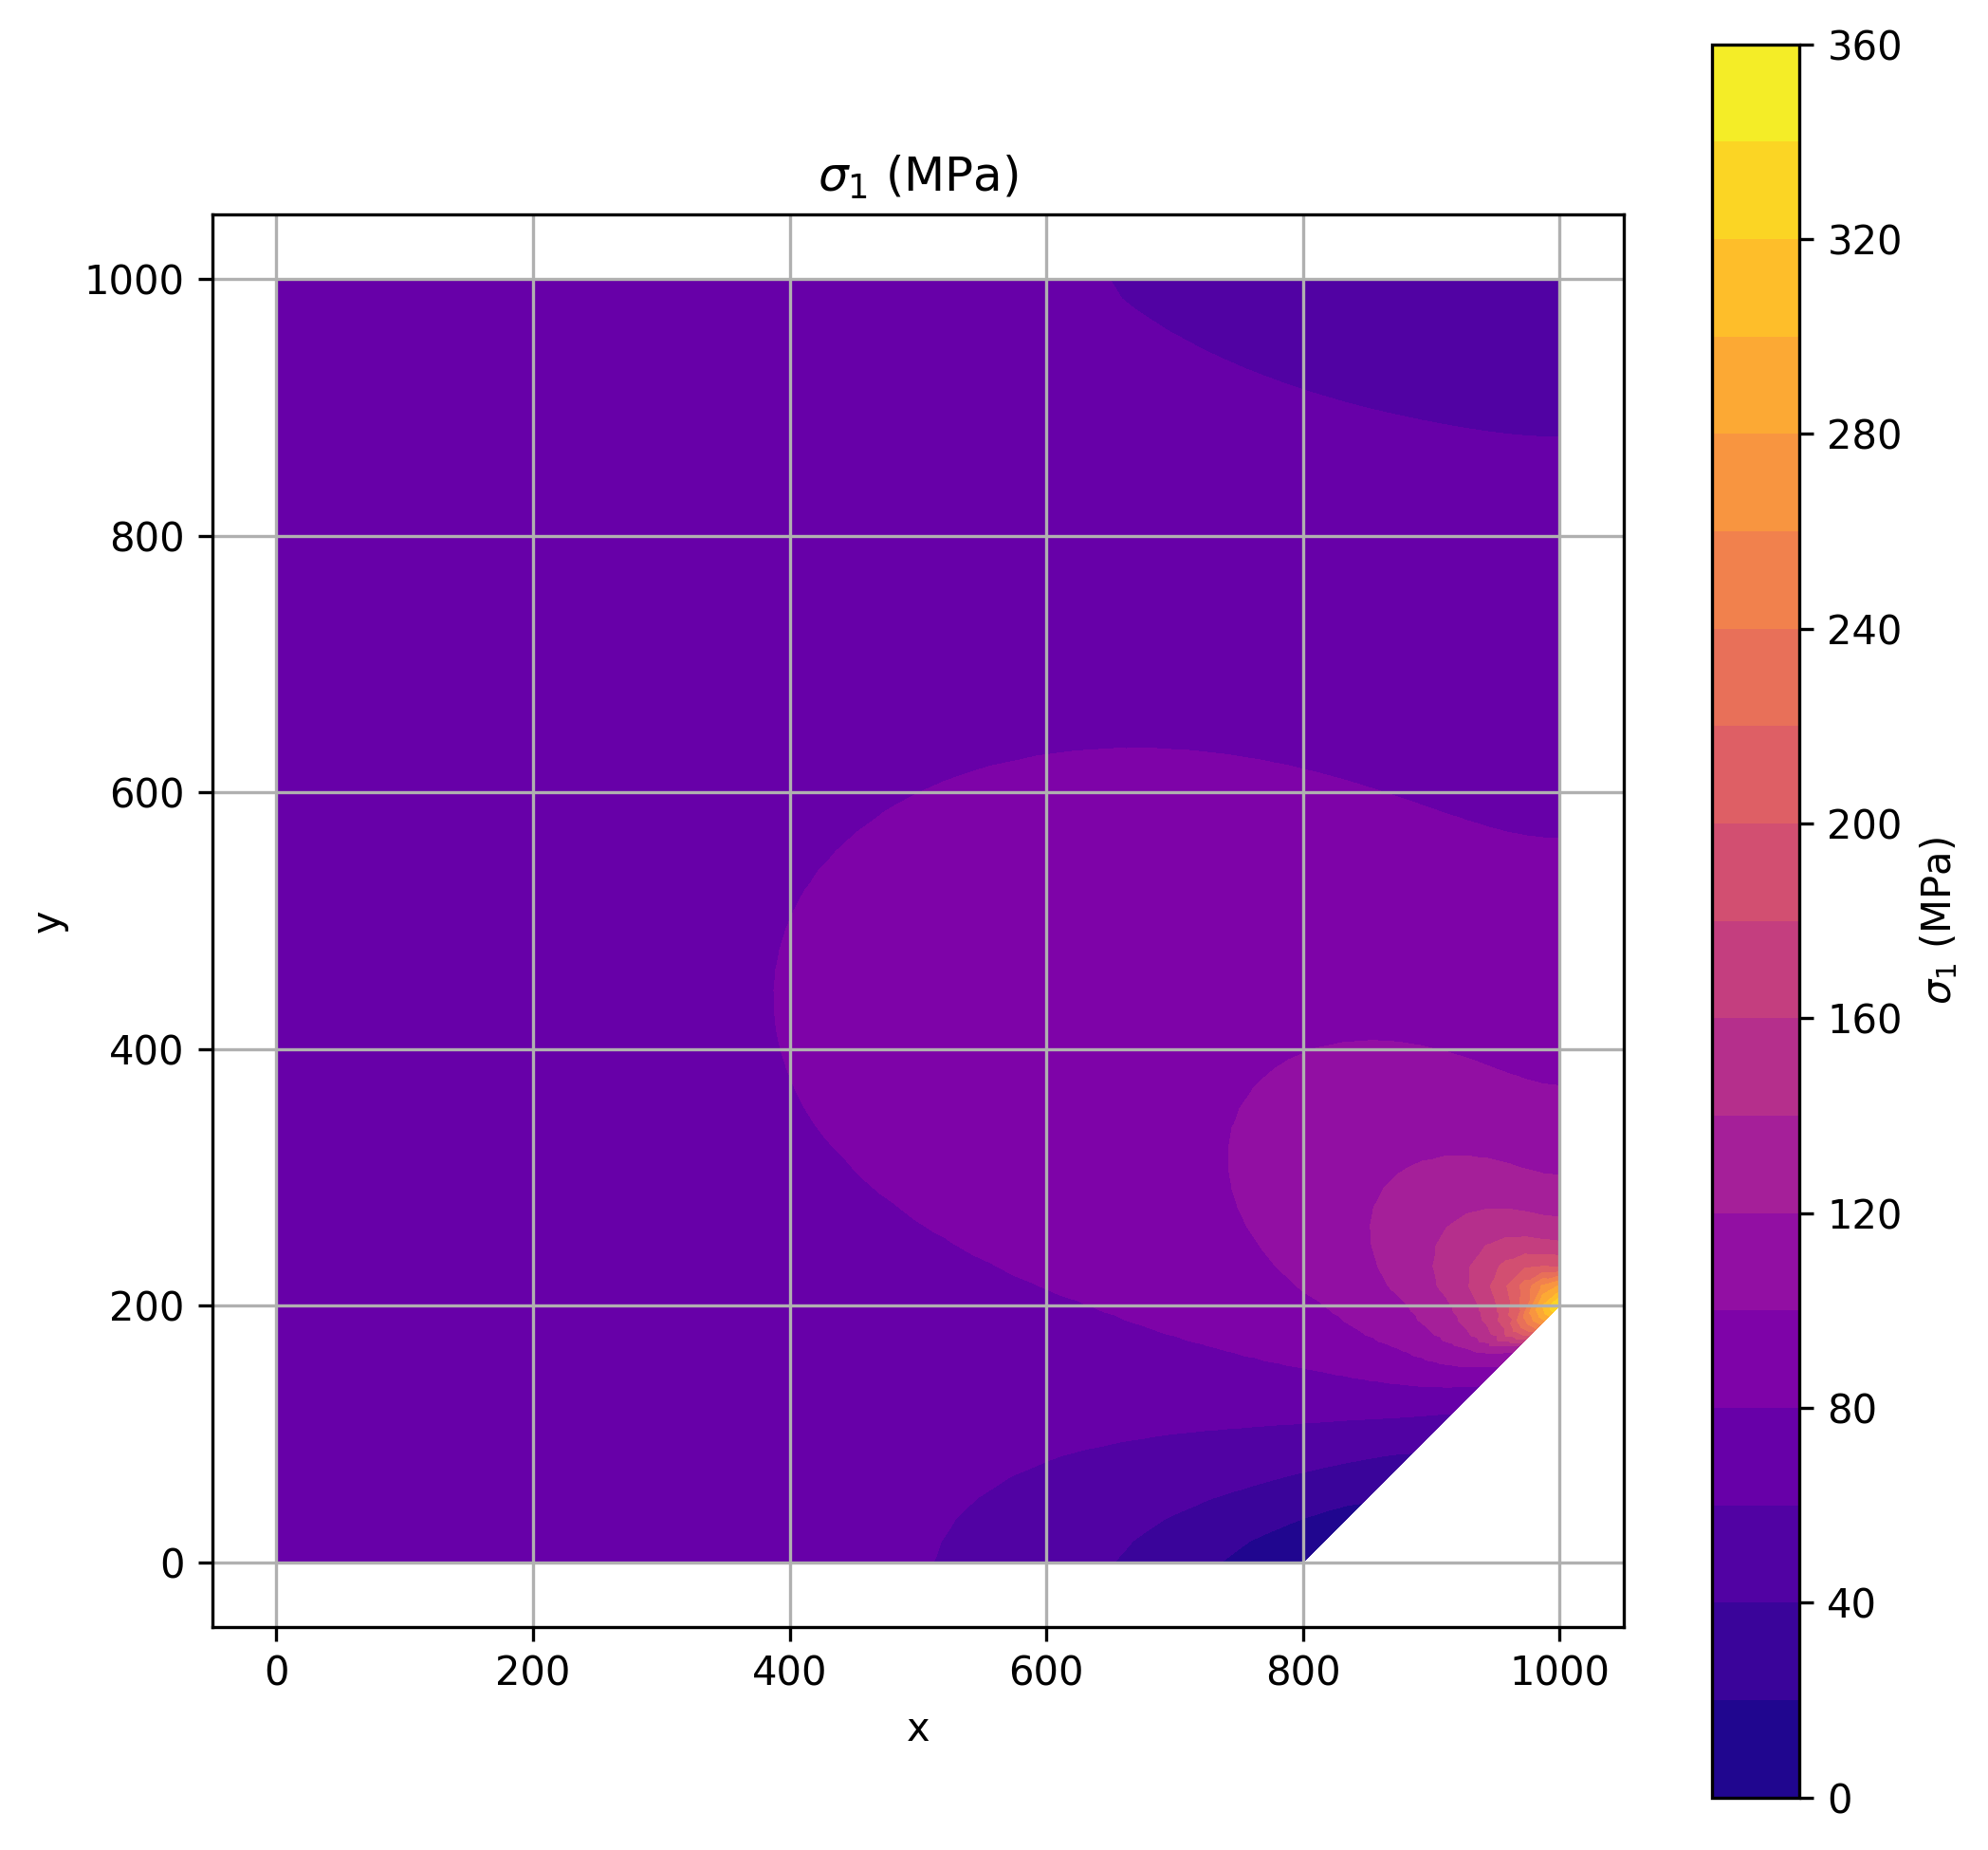
\includegraphics[width=\textwidth]{GRAFICOS/Quad4/1.75mm_local/resultados - sigma_1.png}
    \caption{Local mesh refinement - $h=1.75mm$}
    \label{fig:img21}
  \end{subfigure}
\end{figure}

\begin{figure}[H]
  \centering
  \begin{subfigure}[b]{0.45\textwidth}
    \centering
    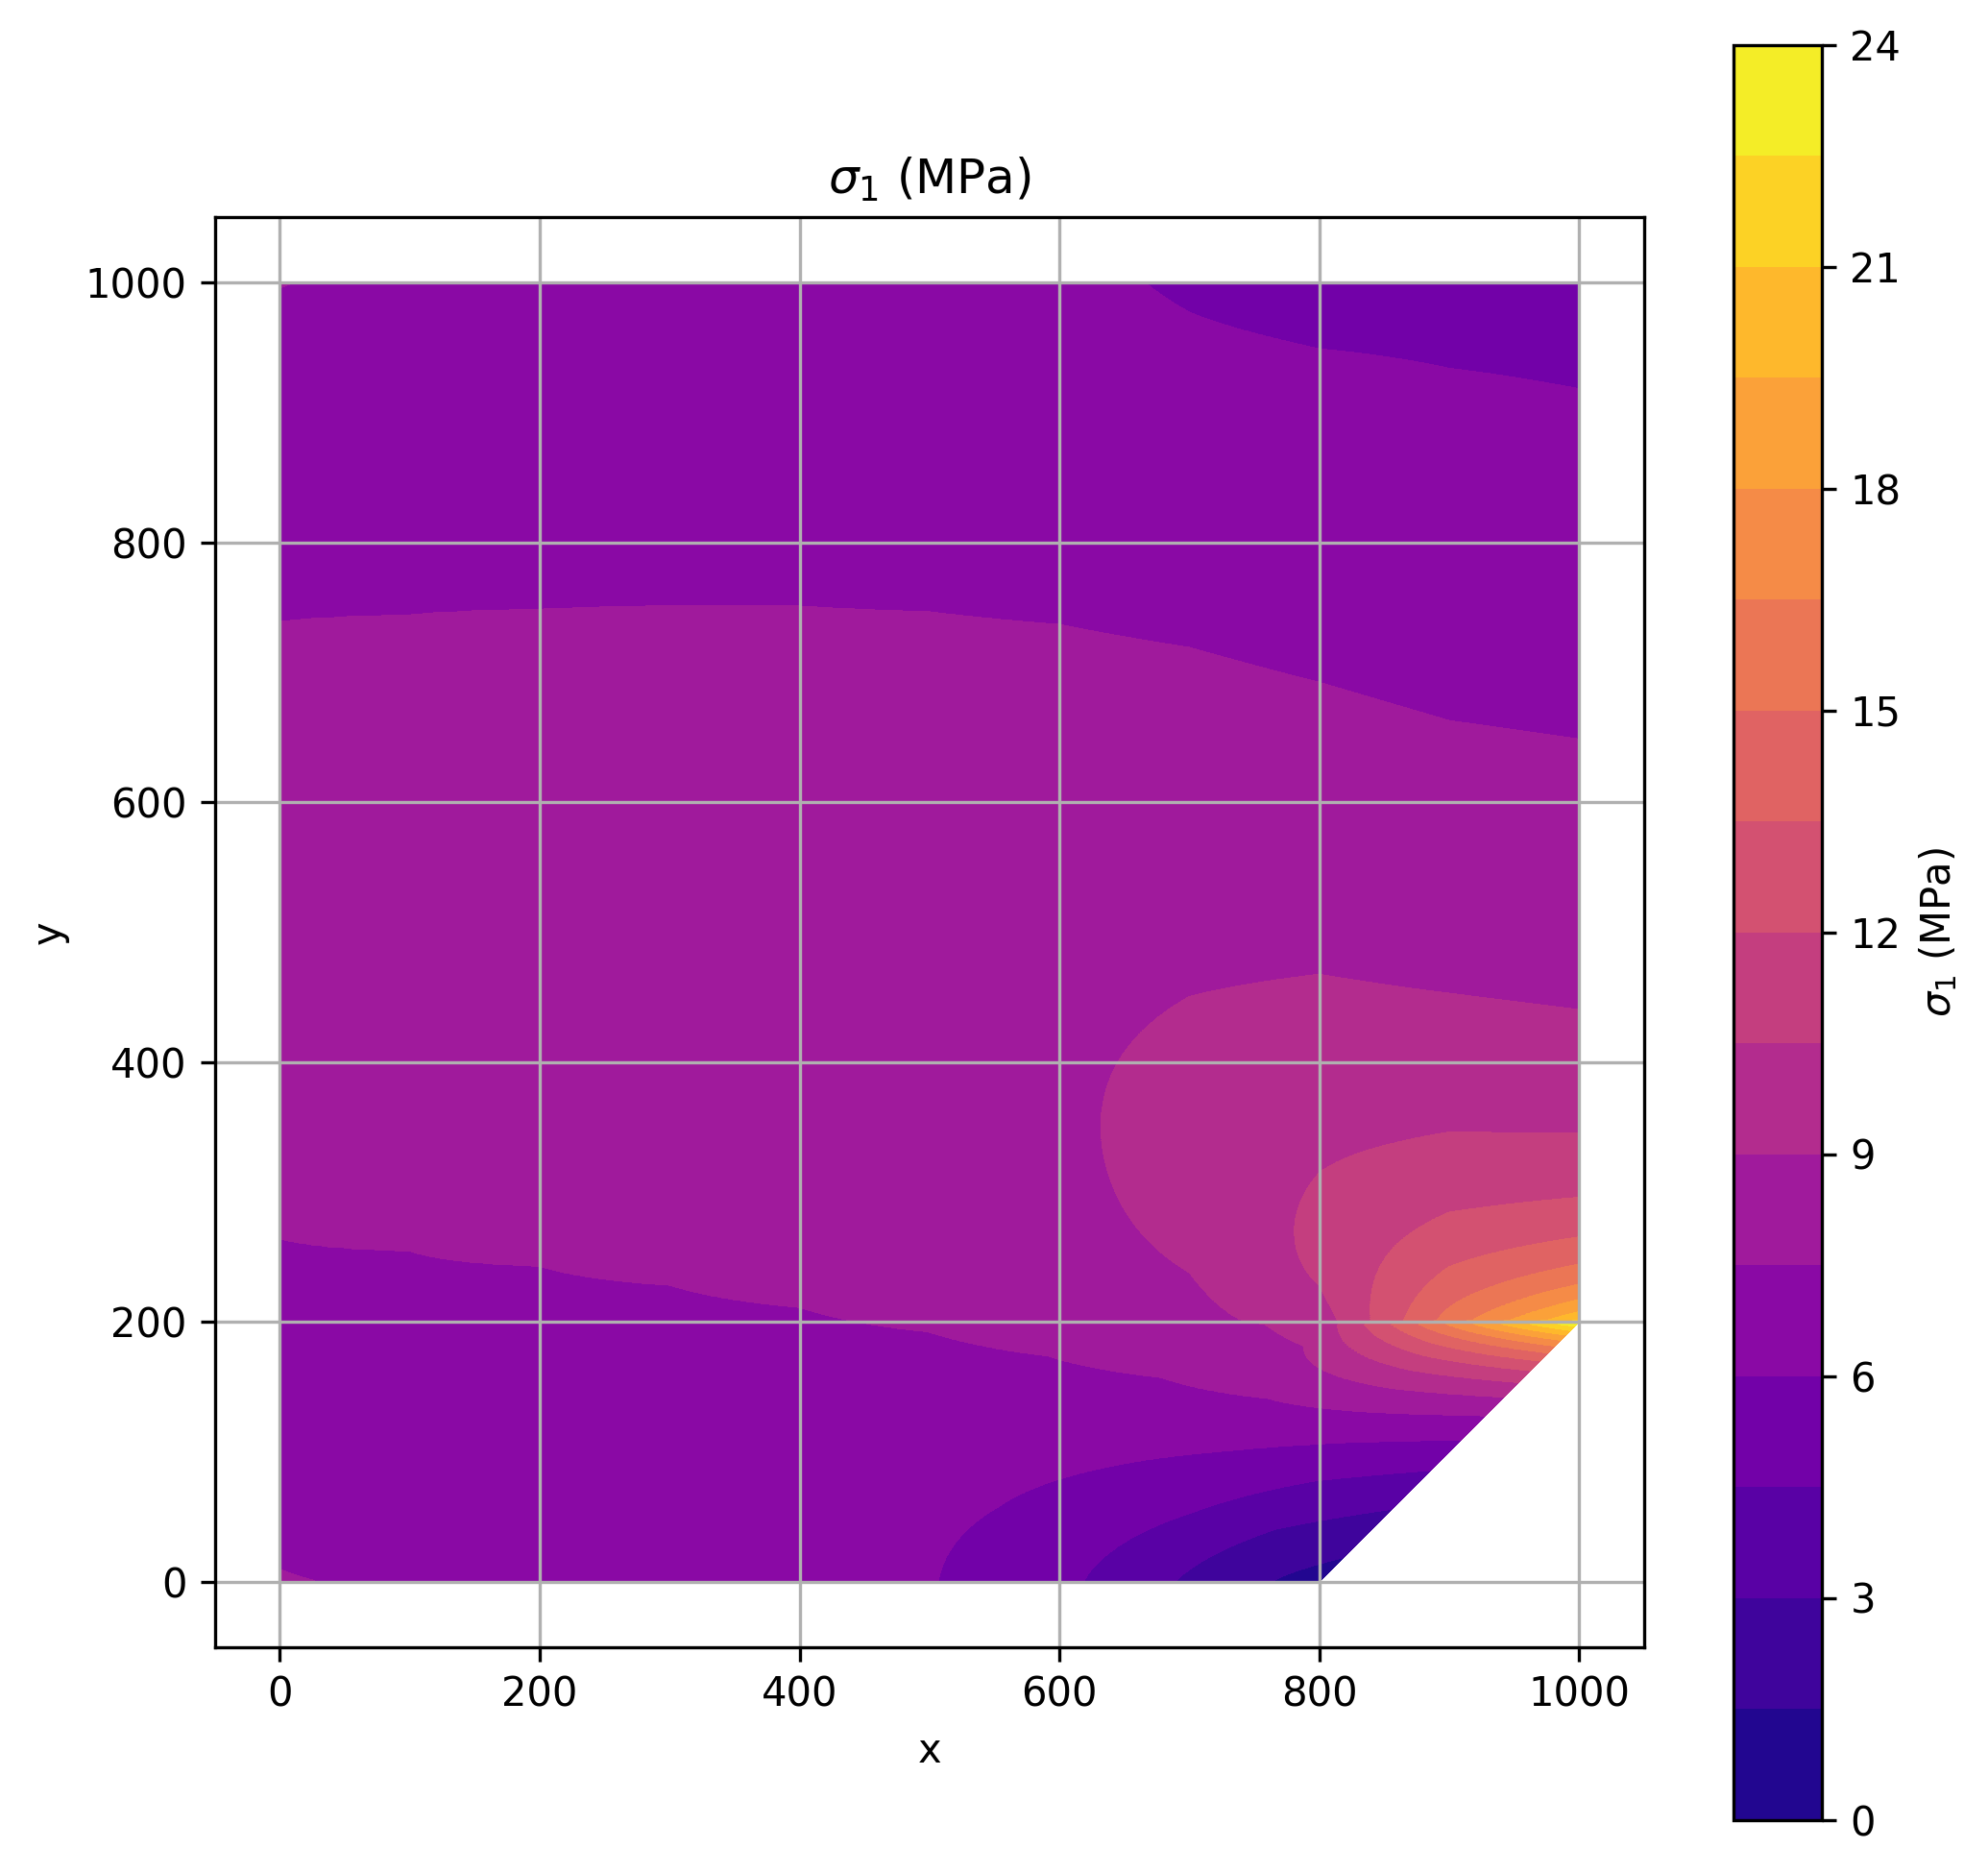
\includegraphics[width=\textwidth]{GRAFICOS/Quad4/1.5mm_global/resultados - sigma_1.png}
    \caption{Global mesh refinement - $h=1.5mm$}
    \label{fig:img12}
  \end{subfigure}
  \hfill
  \begin{subfigure}[b]{0.45\textwidth}
    \centering
    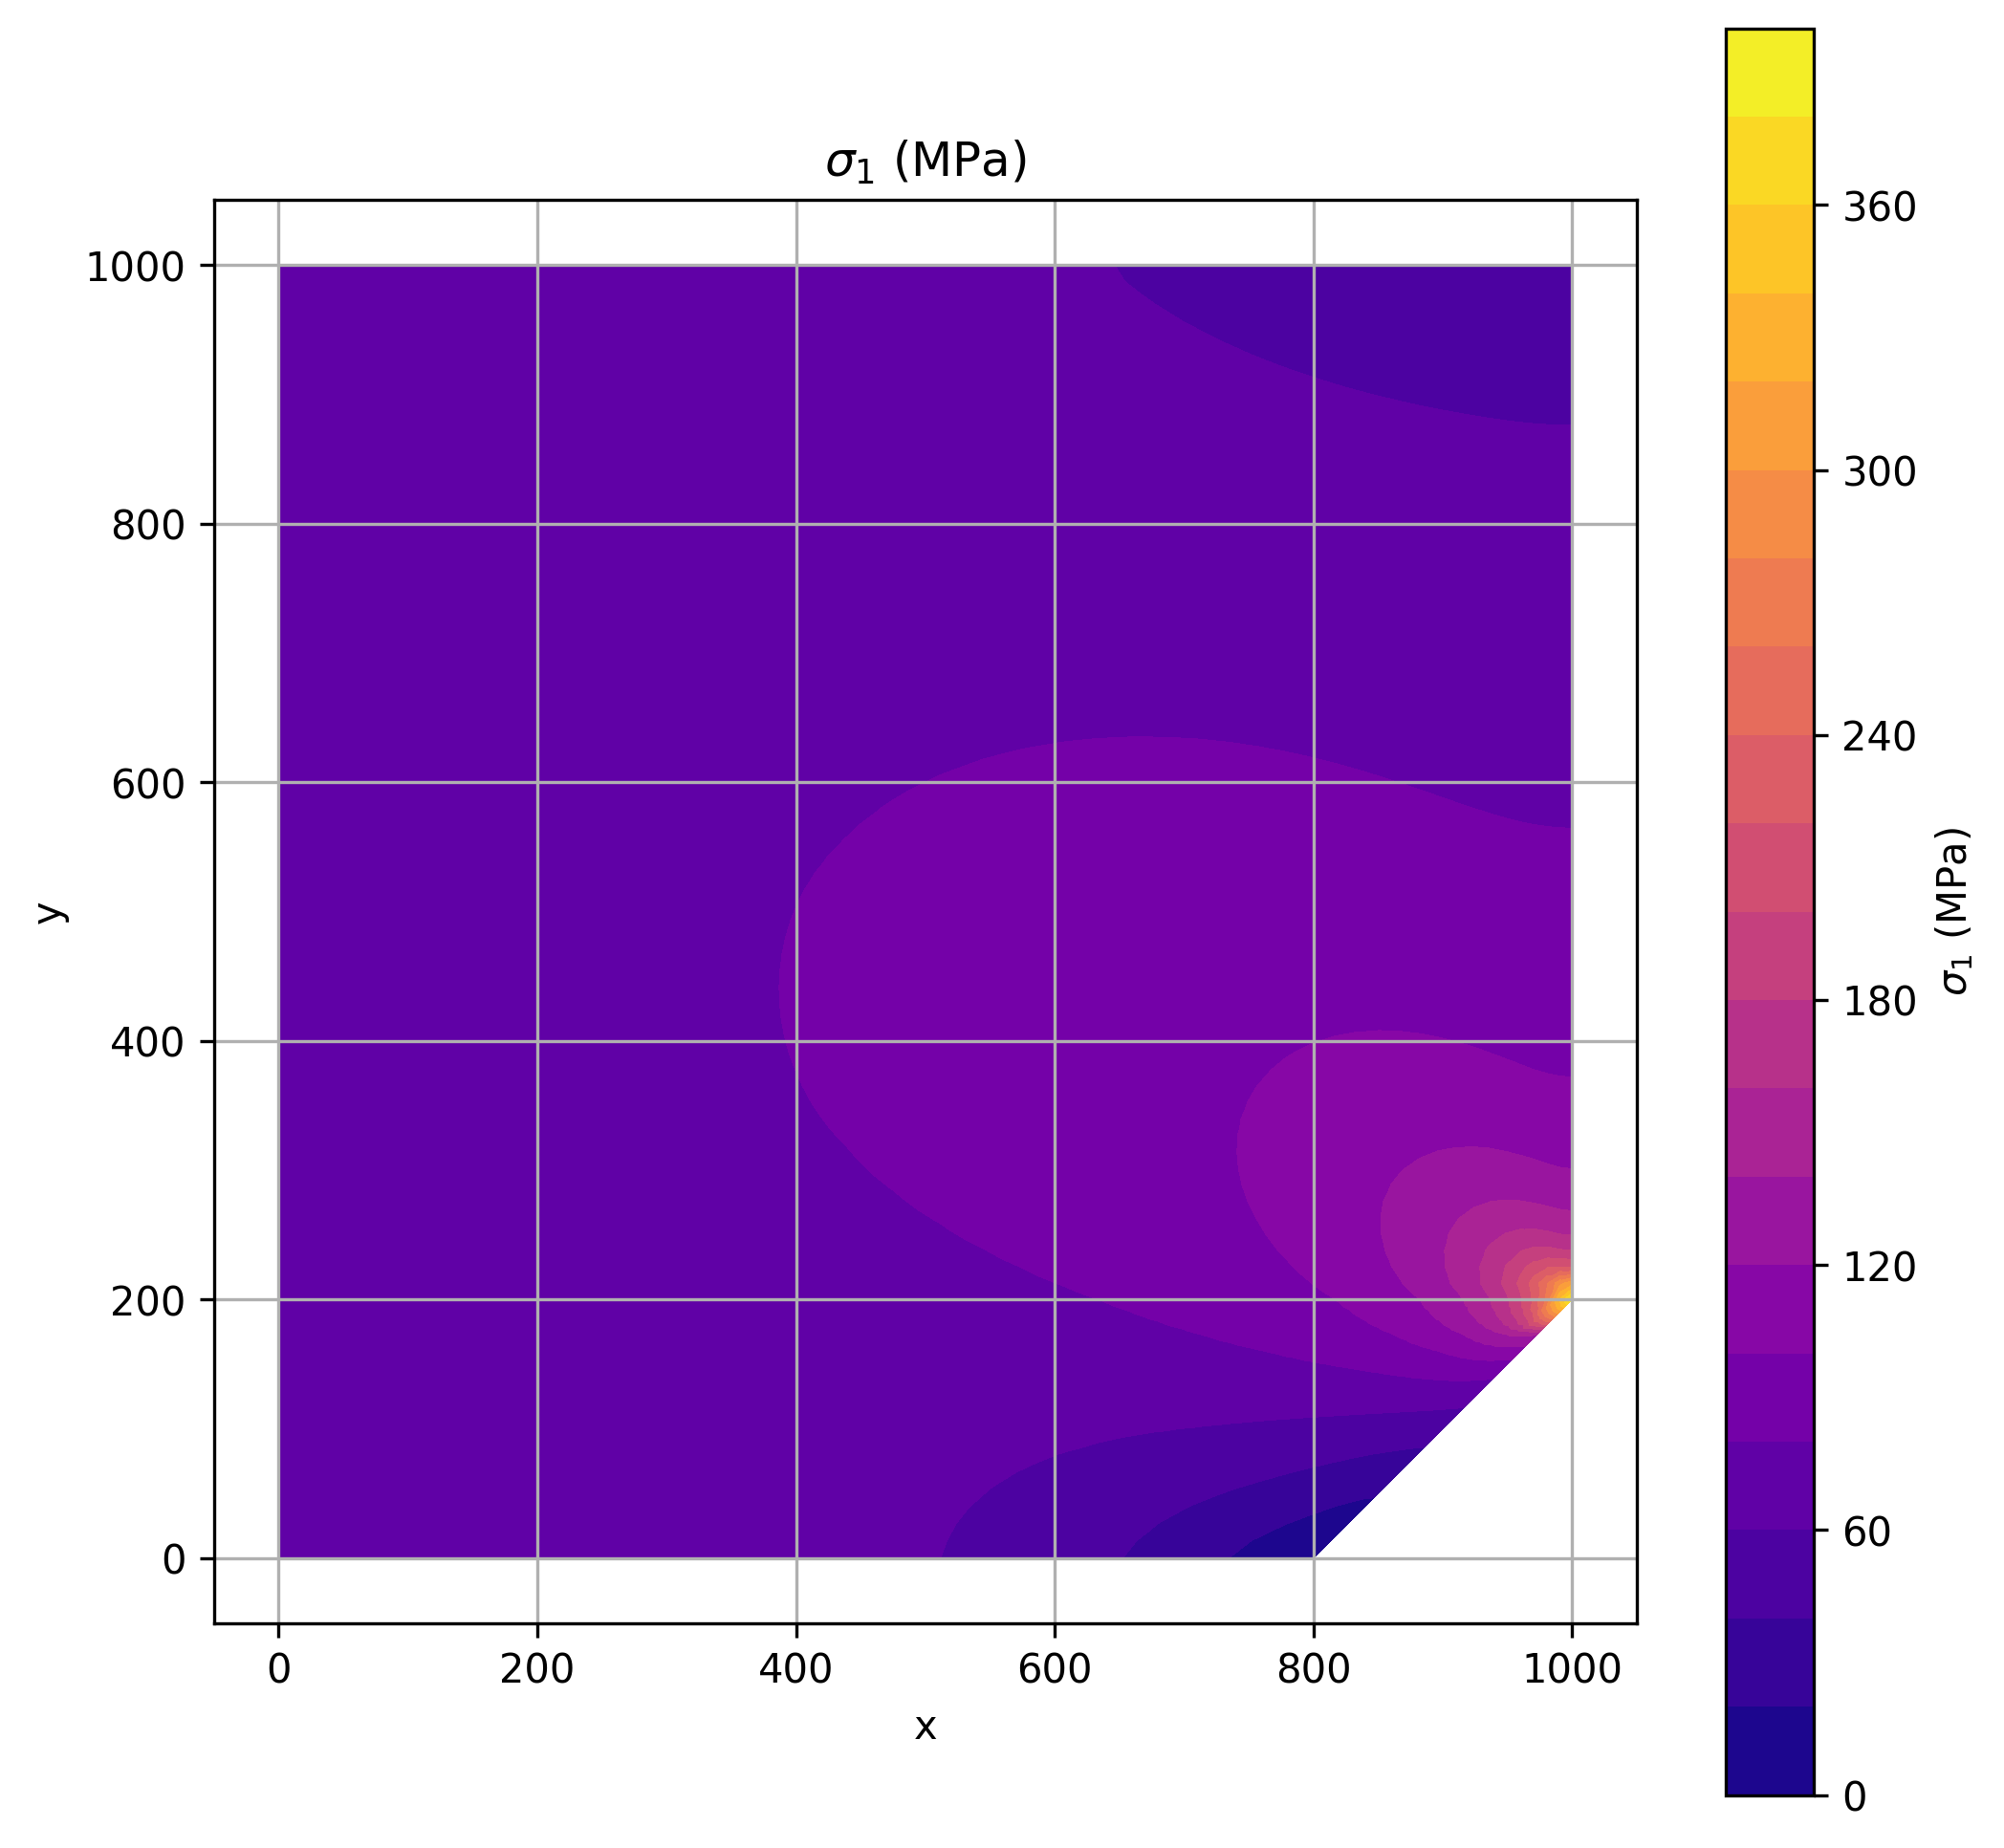
\includegraphics[width=\textwidth]{GRAFICOS/Quad4/1.5mm_local/resultados - sigma_1.png}
    \caption{Local mesh refinement - $h=1.5mm$}
    \label{fig:img22}
  \end{subfigure}
\end{figure}

\begin{figure}[H]
  \centering
  \begin{subfigure}[b]{0.45\textwidth}
    \centering
    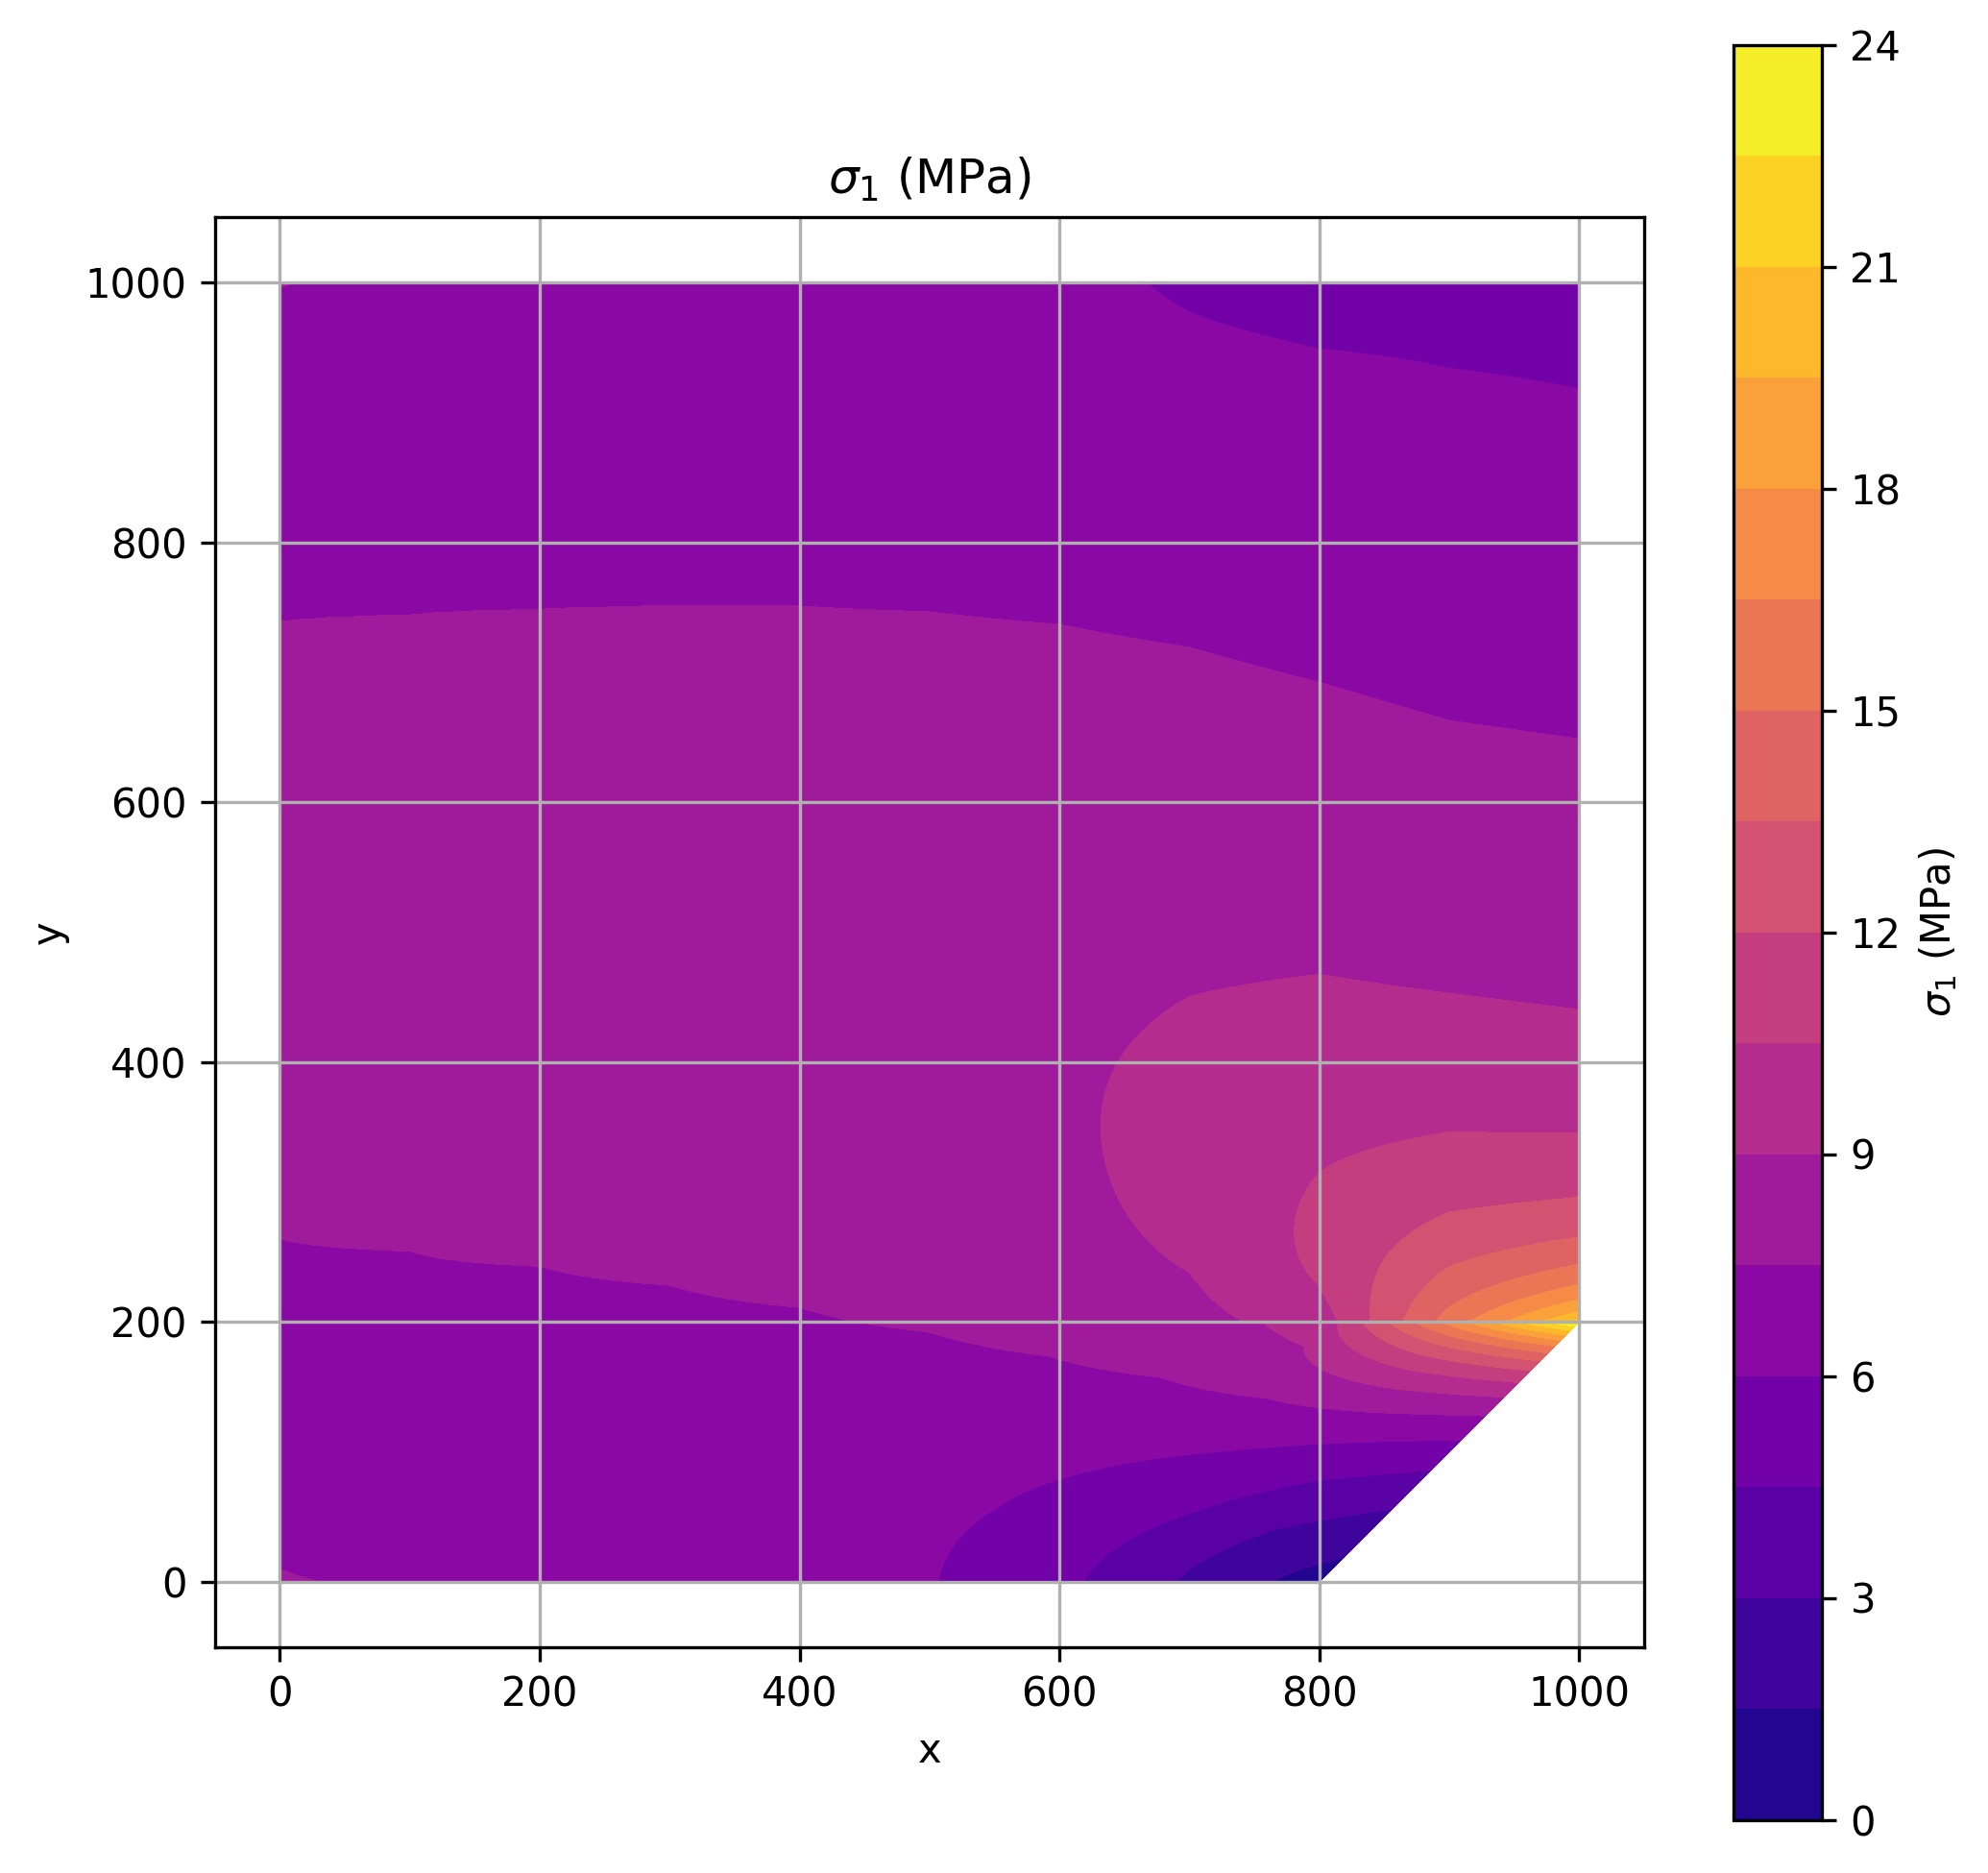
\includegraphics[width=\textwidth]{GRAFICOS/Quad4/1.25mm_global/resultados - sigma_1.png}
    \caption{Global mesh refinement - $h=1.25mm$}
    \label{fig:img13}
  \end{subfigure}
  \hfill
  \begin{subfigure}[b]{0.45\textwidth}
    \centering
    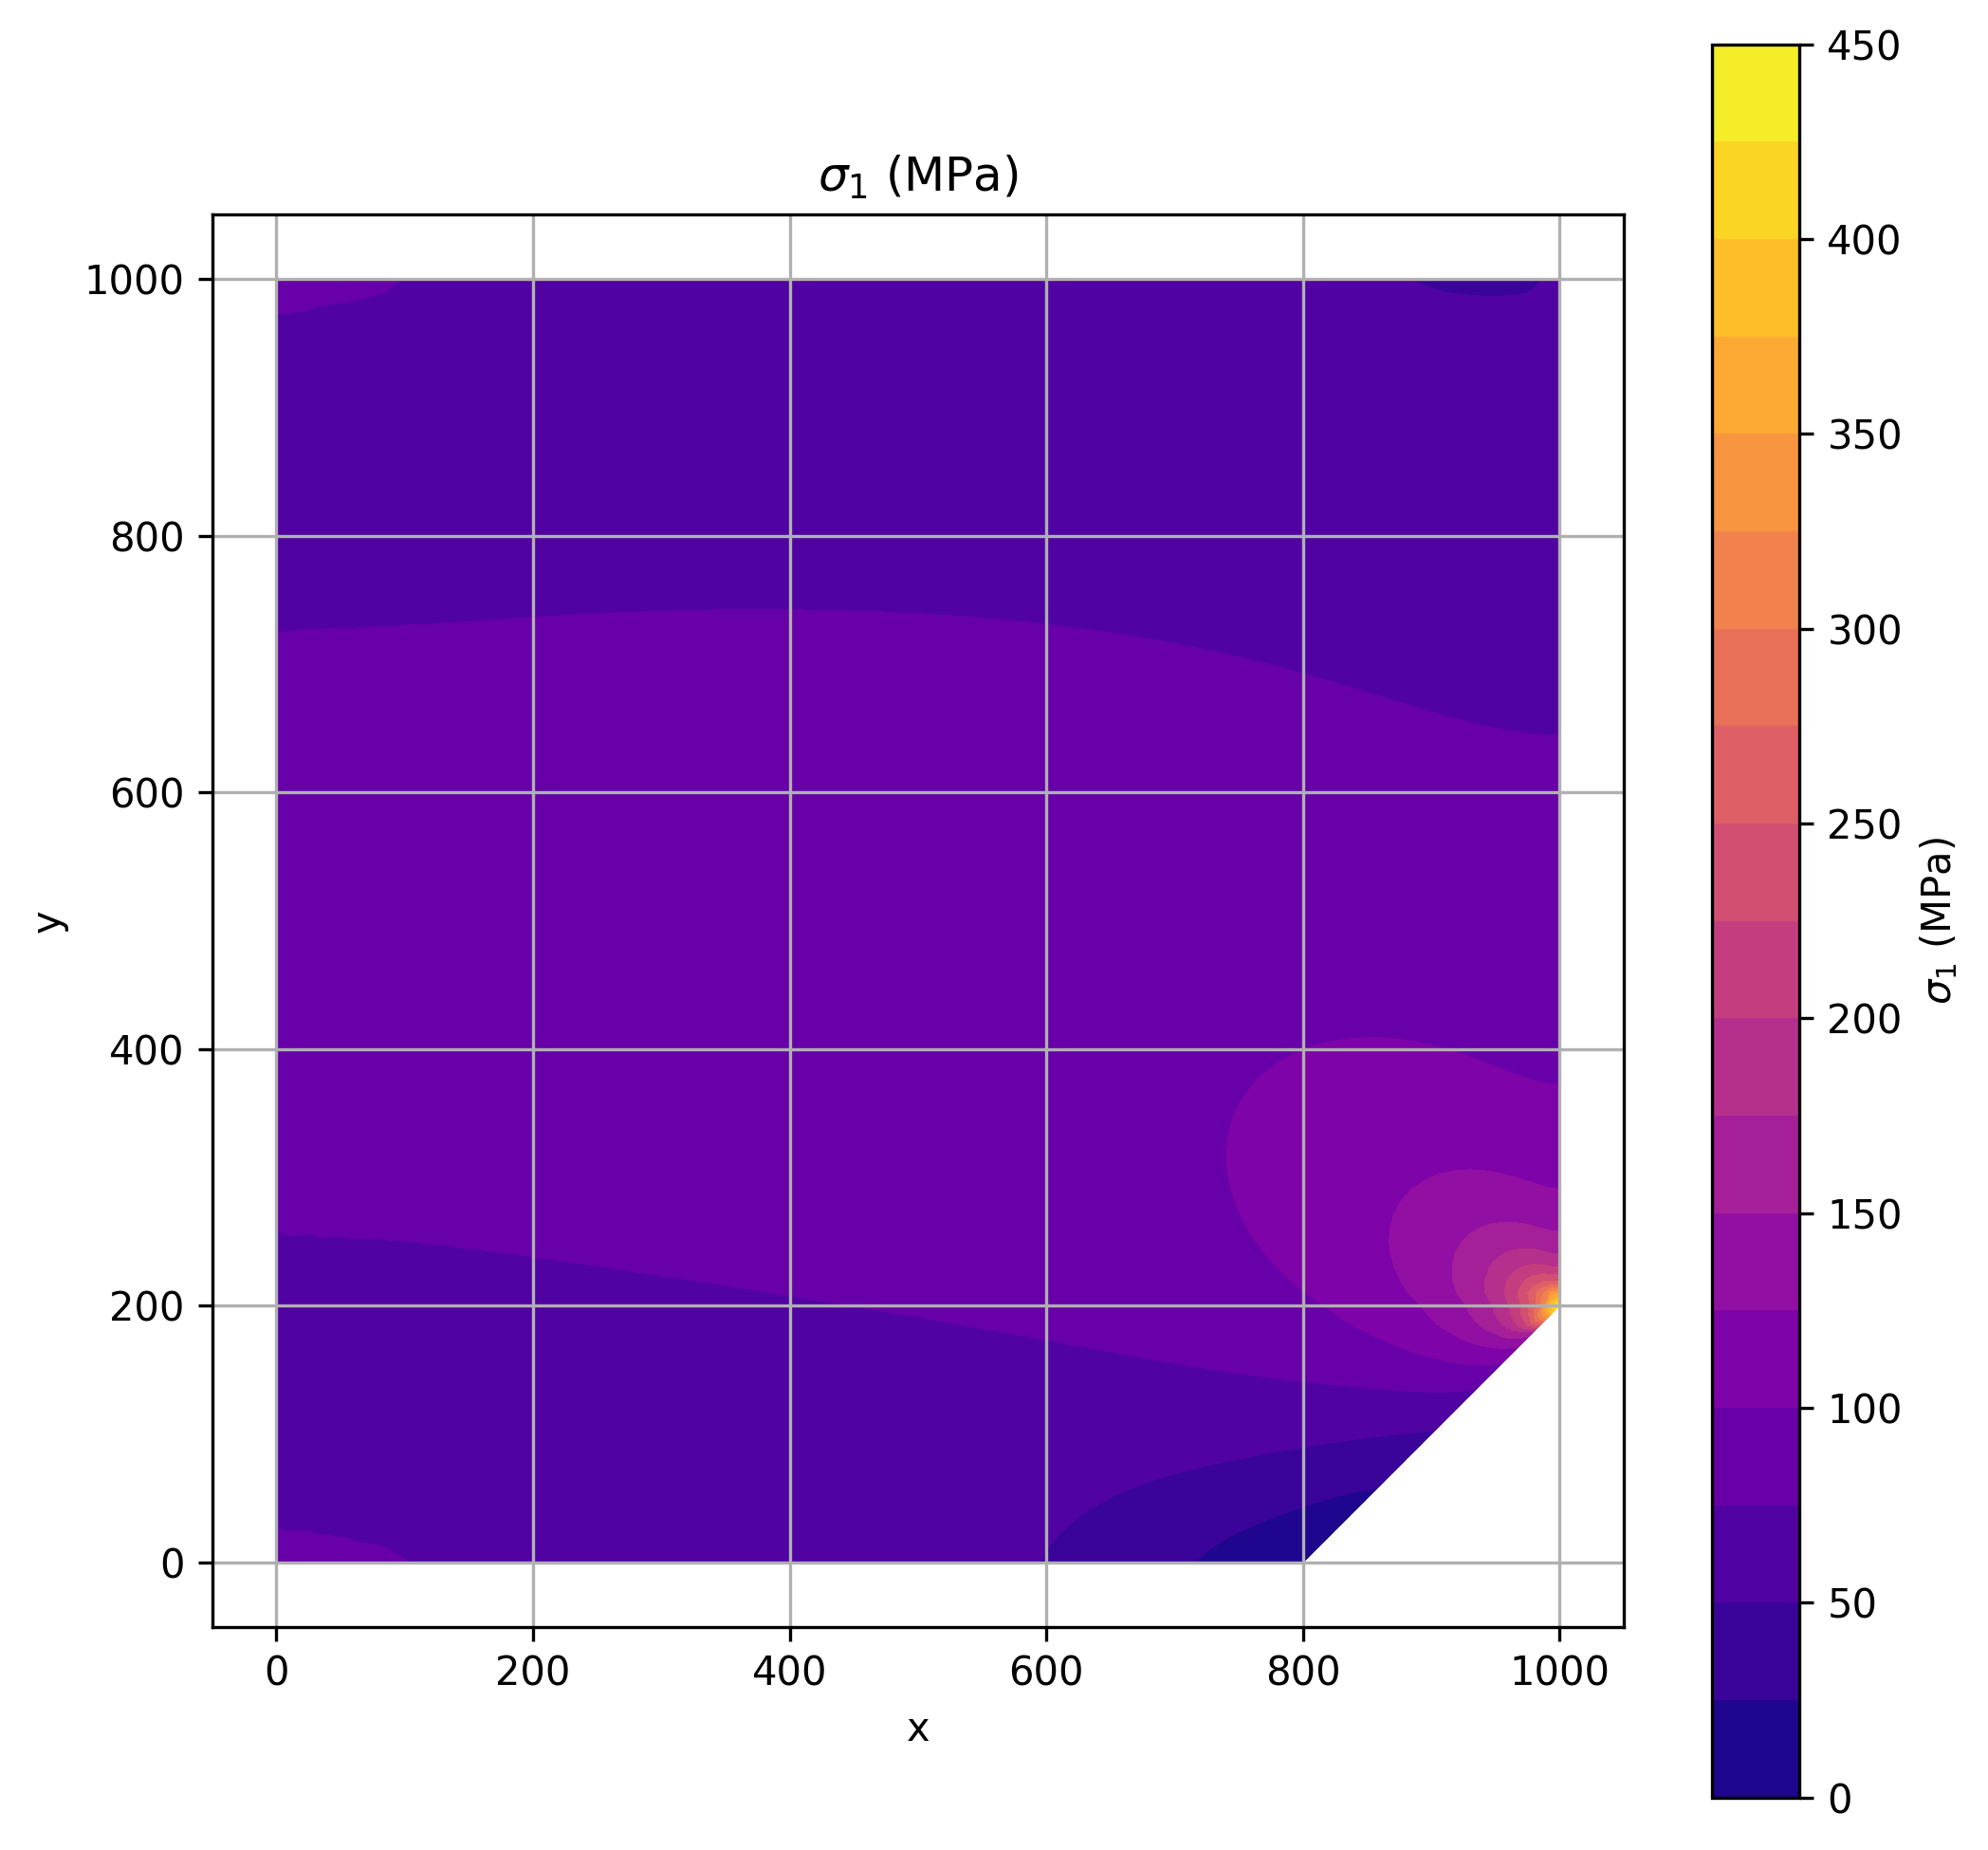
\includegraphics[width=\textwidth]{GRAFICOS/Quad4/1.25mm_local/resultados - sigma_1.png}
    \caption{Local mesh refinement - $h=1.25mm$}
    \label{fig:img23}
  \end{subfigure}
\end{figure}

\begin{table}[H]
  \centering
\caption{Table of $\sigma_{\max}$ with global and local refinement for different $h$ - Quad4 Elements}
  \begin{tabular}{|c|c|c|}
    \hline
    \multicolumn{3}{|c|}{$\sigma_{max} (MPa)$} \\ \hline
    $h$ (mm) & Global & Local \\ \hline
    2 & 236.13 & 282.74 \\ \hline
    1.75 & 260.26 & 320.69 \\ \hline
    1.5 & 284.55 & 360.88 \\ \hline
    1.25 & 313.78 & 409.92 \\ \hline
  \end{tabular}
  \label{tab:5x2}
\end{table}

\subsubsection{Quad9 Element}

In this section, the same procedure was followed, but increasing the order of the mesh elements to Quad9.

\begin{figure}[H]
  \centering
  \begin{subfigure}[b]{0.45\textwidth}
    \centering
    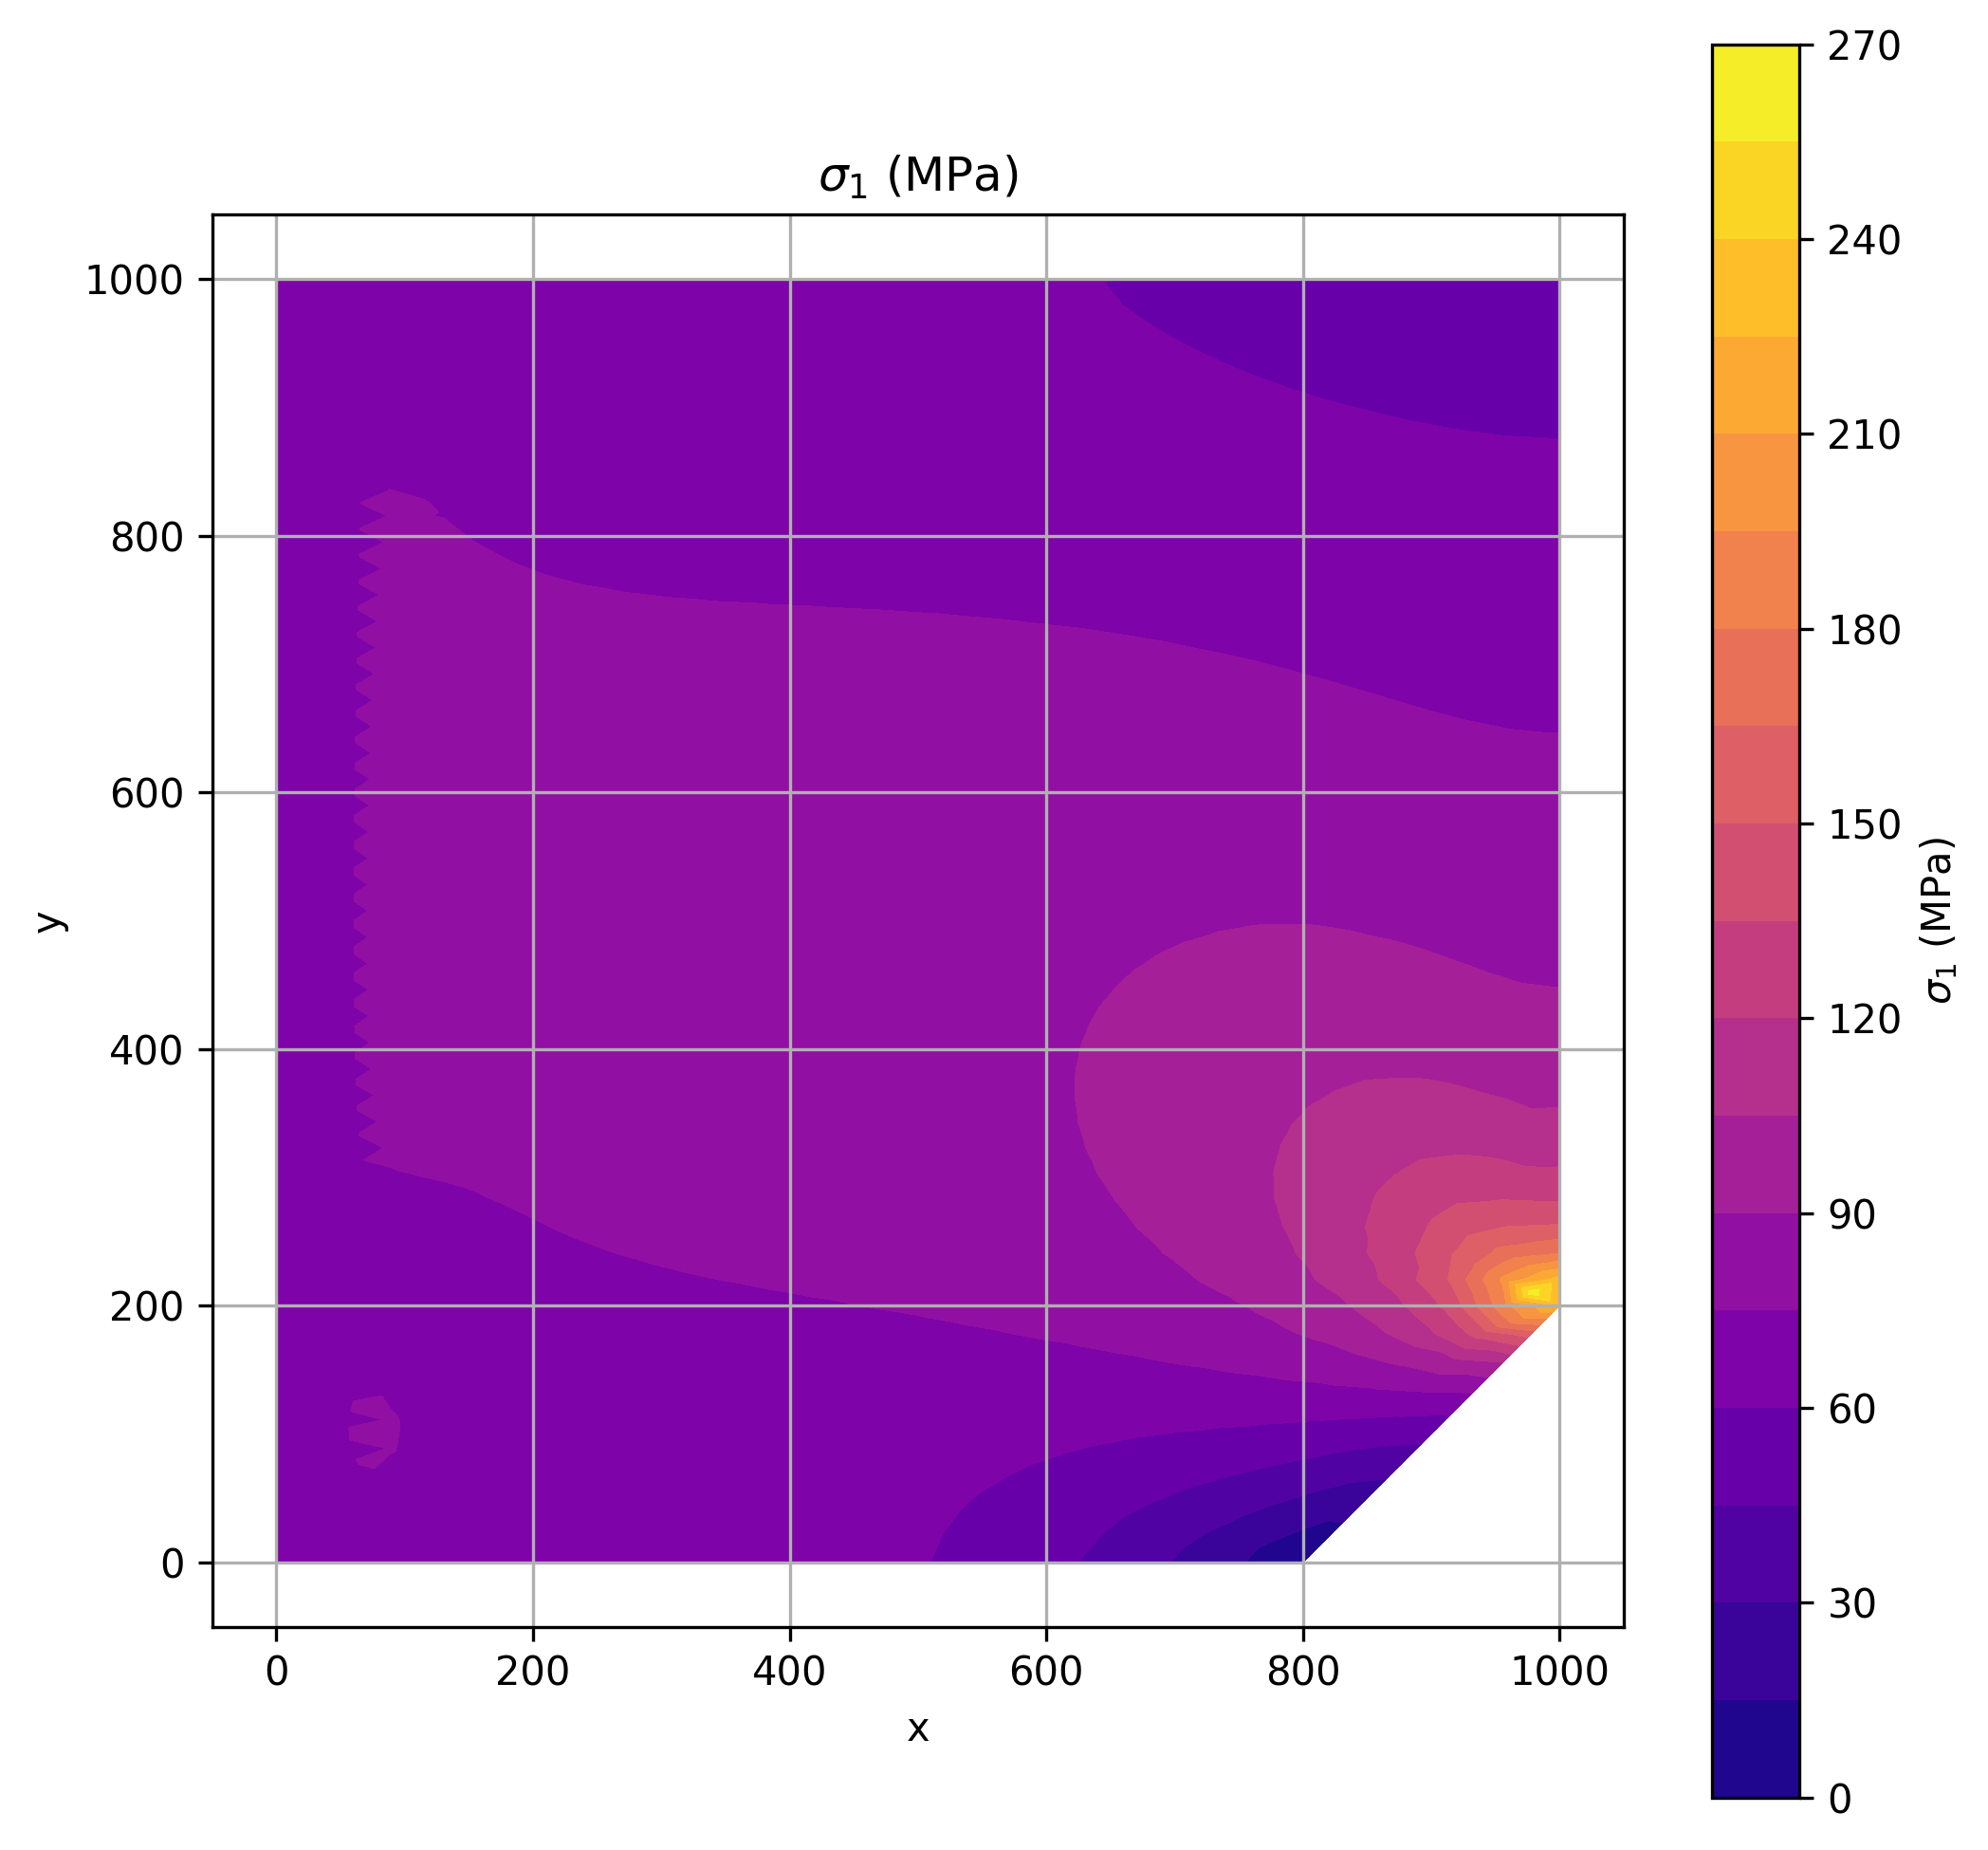
\includegraphics[width=\textwidth]{GRAFICOS/Quad9/2mm_global/resultados - sigma_1.png}
    \caption{Global mesh refinement - $h=2mm$}
    \label{fig:img1}
  \end{subfigure}
  \hfill
  \begin{subfigure}[b]{0.45\textwidth}
    \centering
    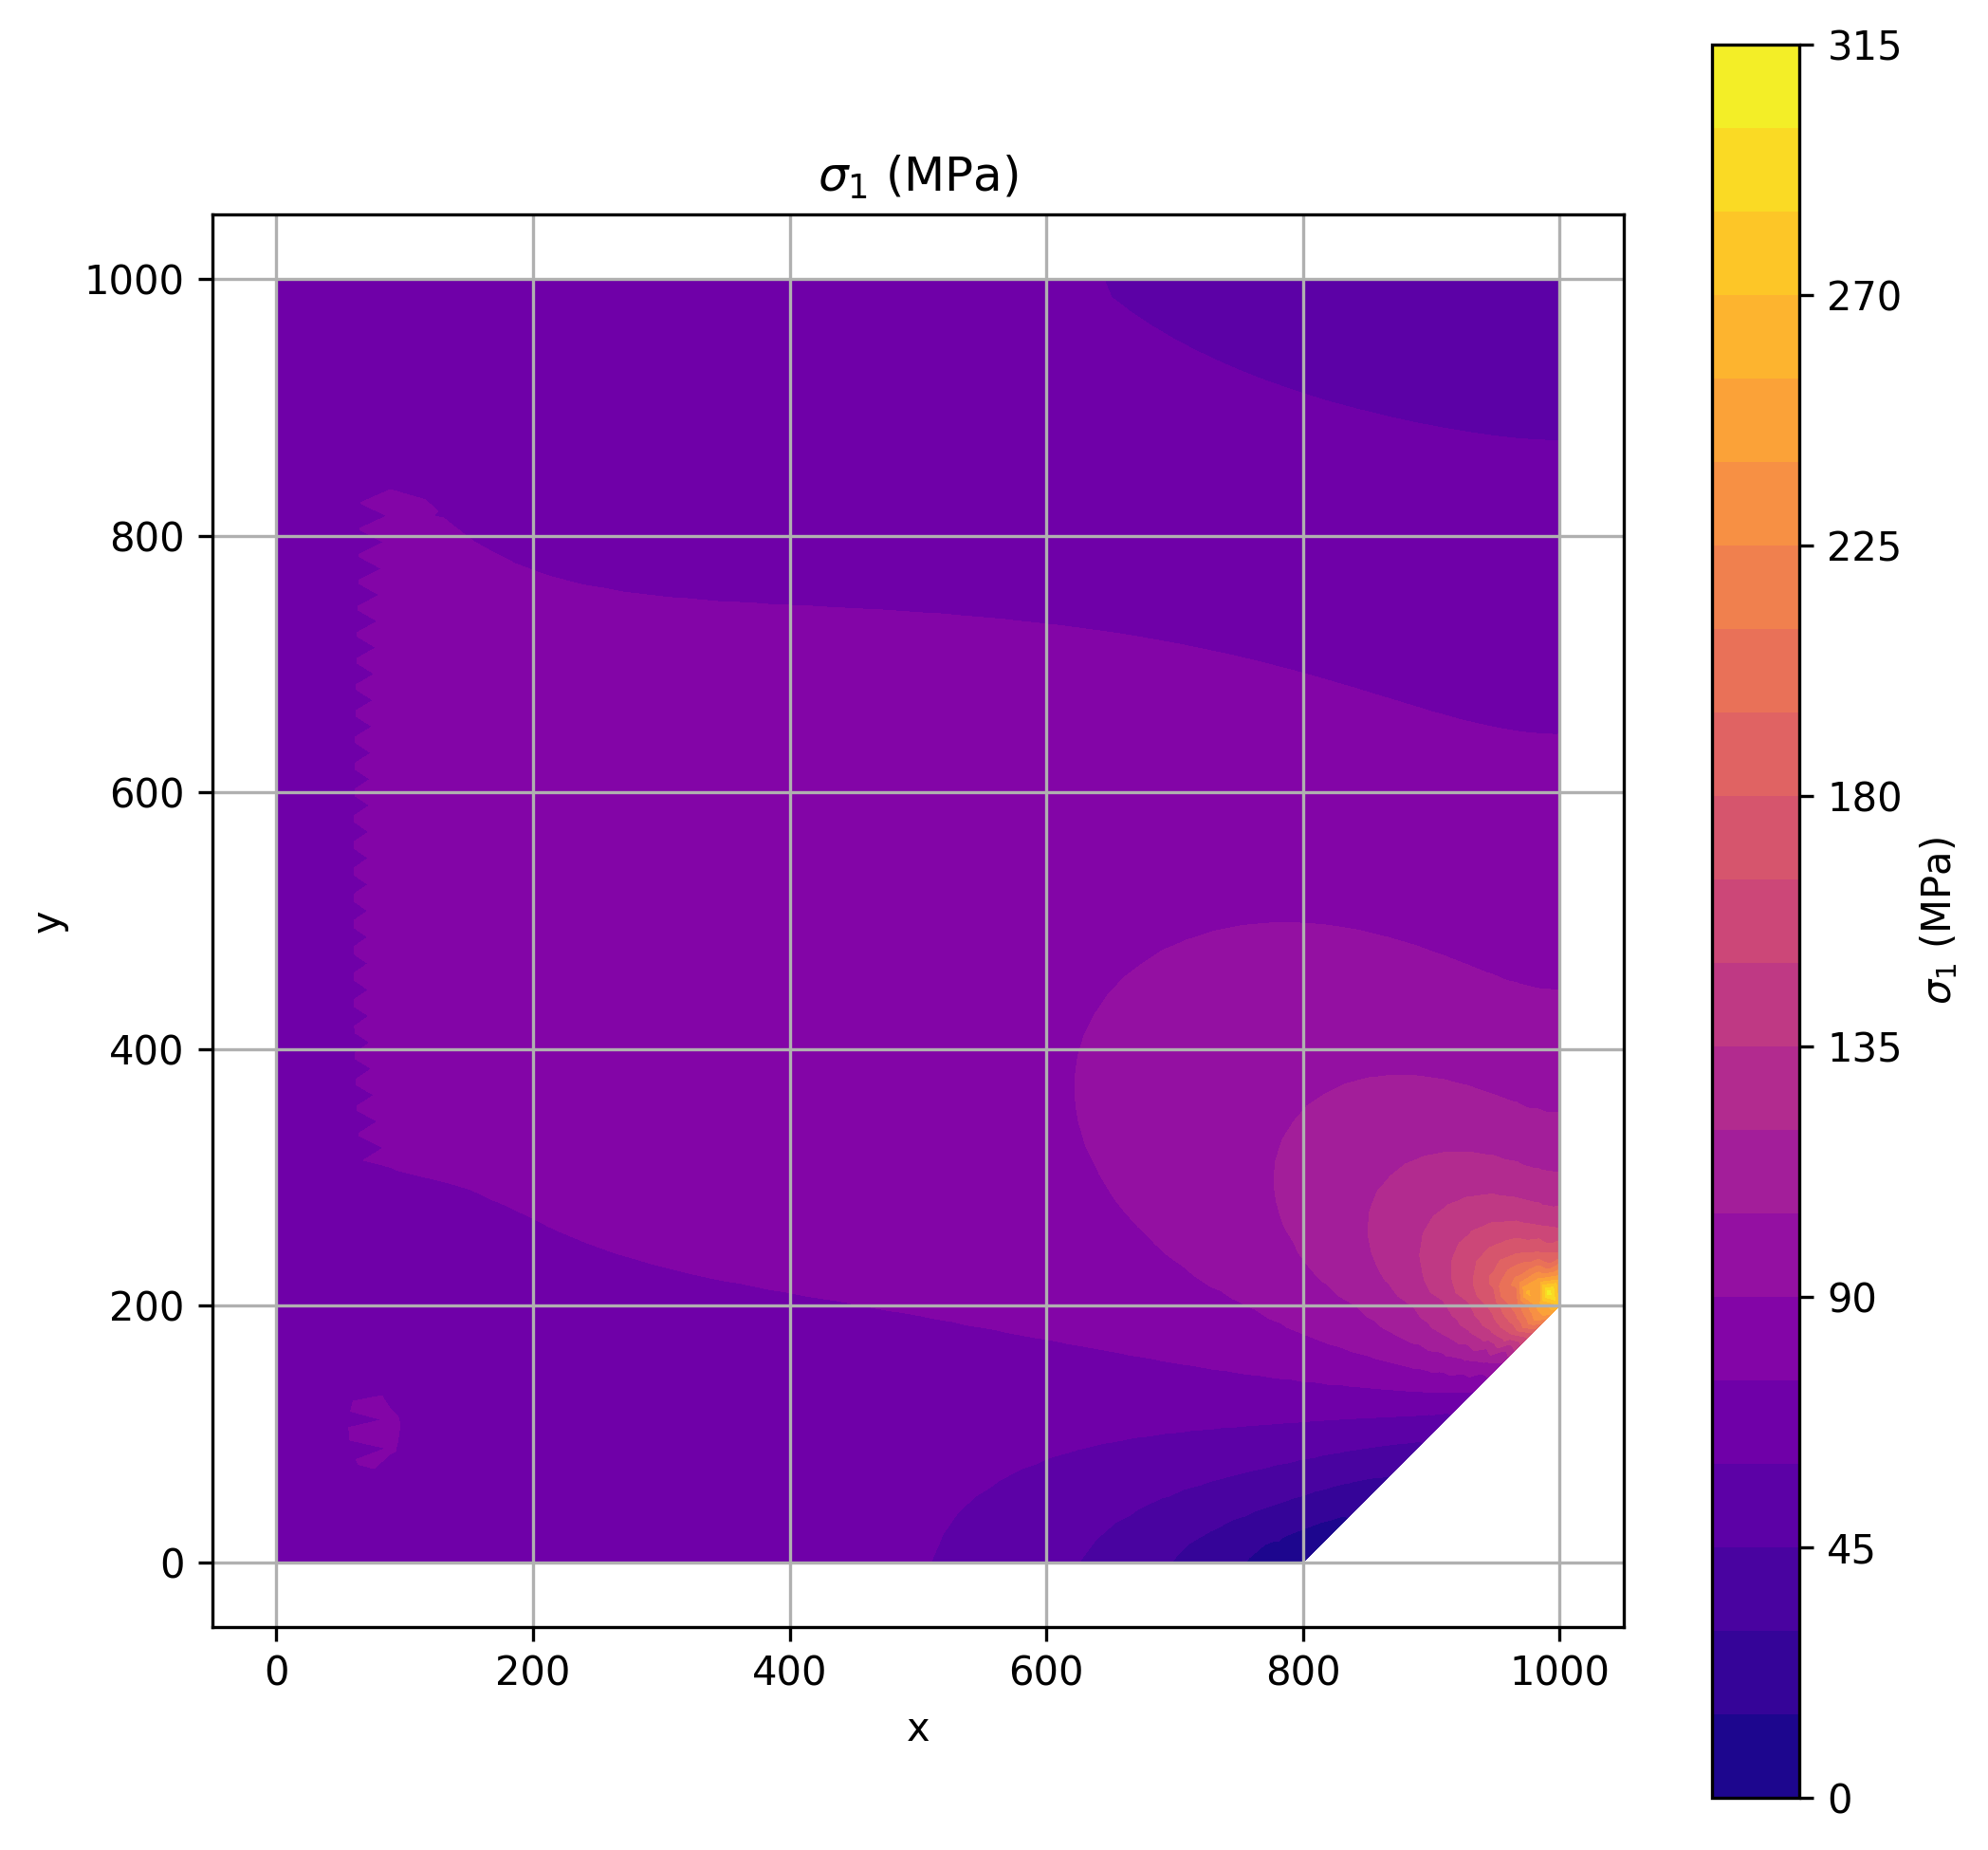
\includegraphics[width=\textwidth]{GRAFICOS/Quad9/2mm_local/resultados - sigma_1.png}
    \caption{Local mesh refinement - $h=2mm$}
    \label{fig:img2}
  \end{subfigure}
\end{figure}

\begin{figure}[H]
  \centering
  \begin{subfigure}[b]{0.45\textwidth}
    \centering
    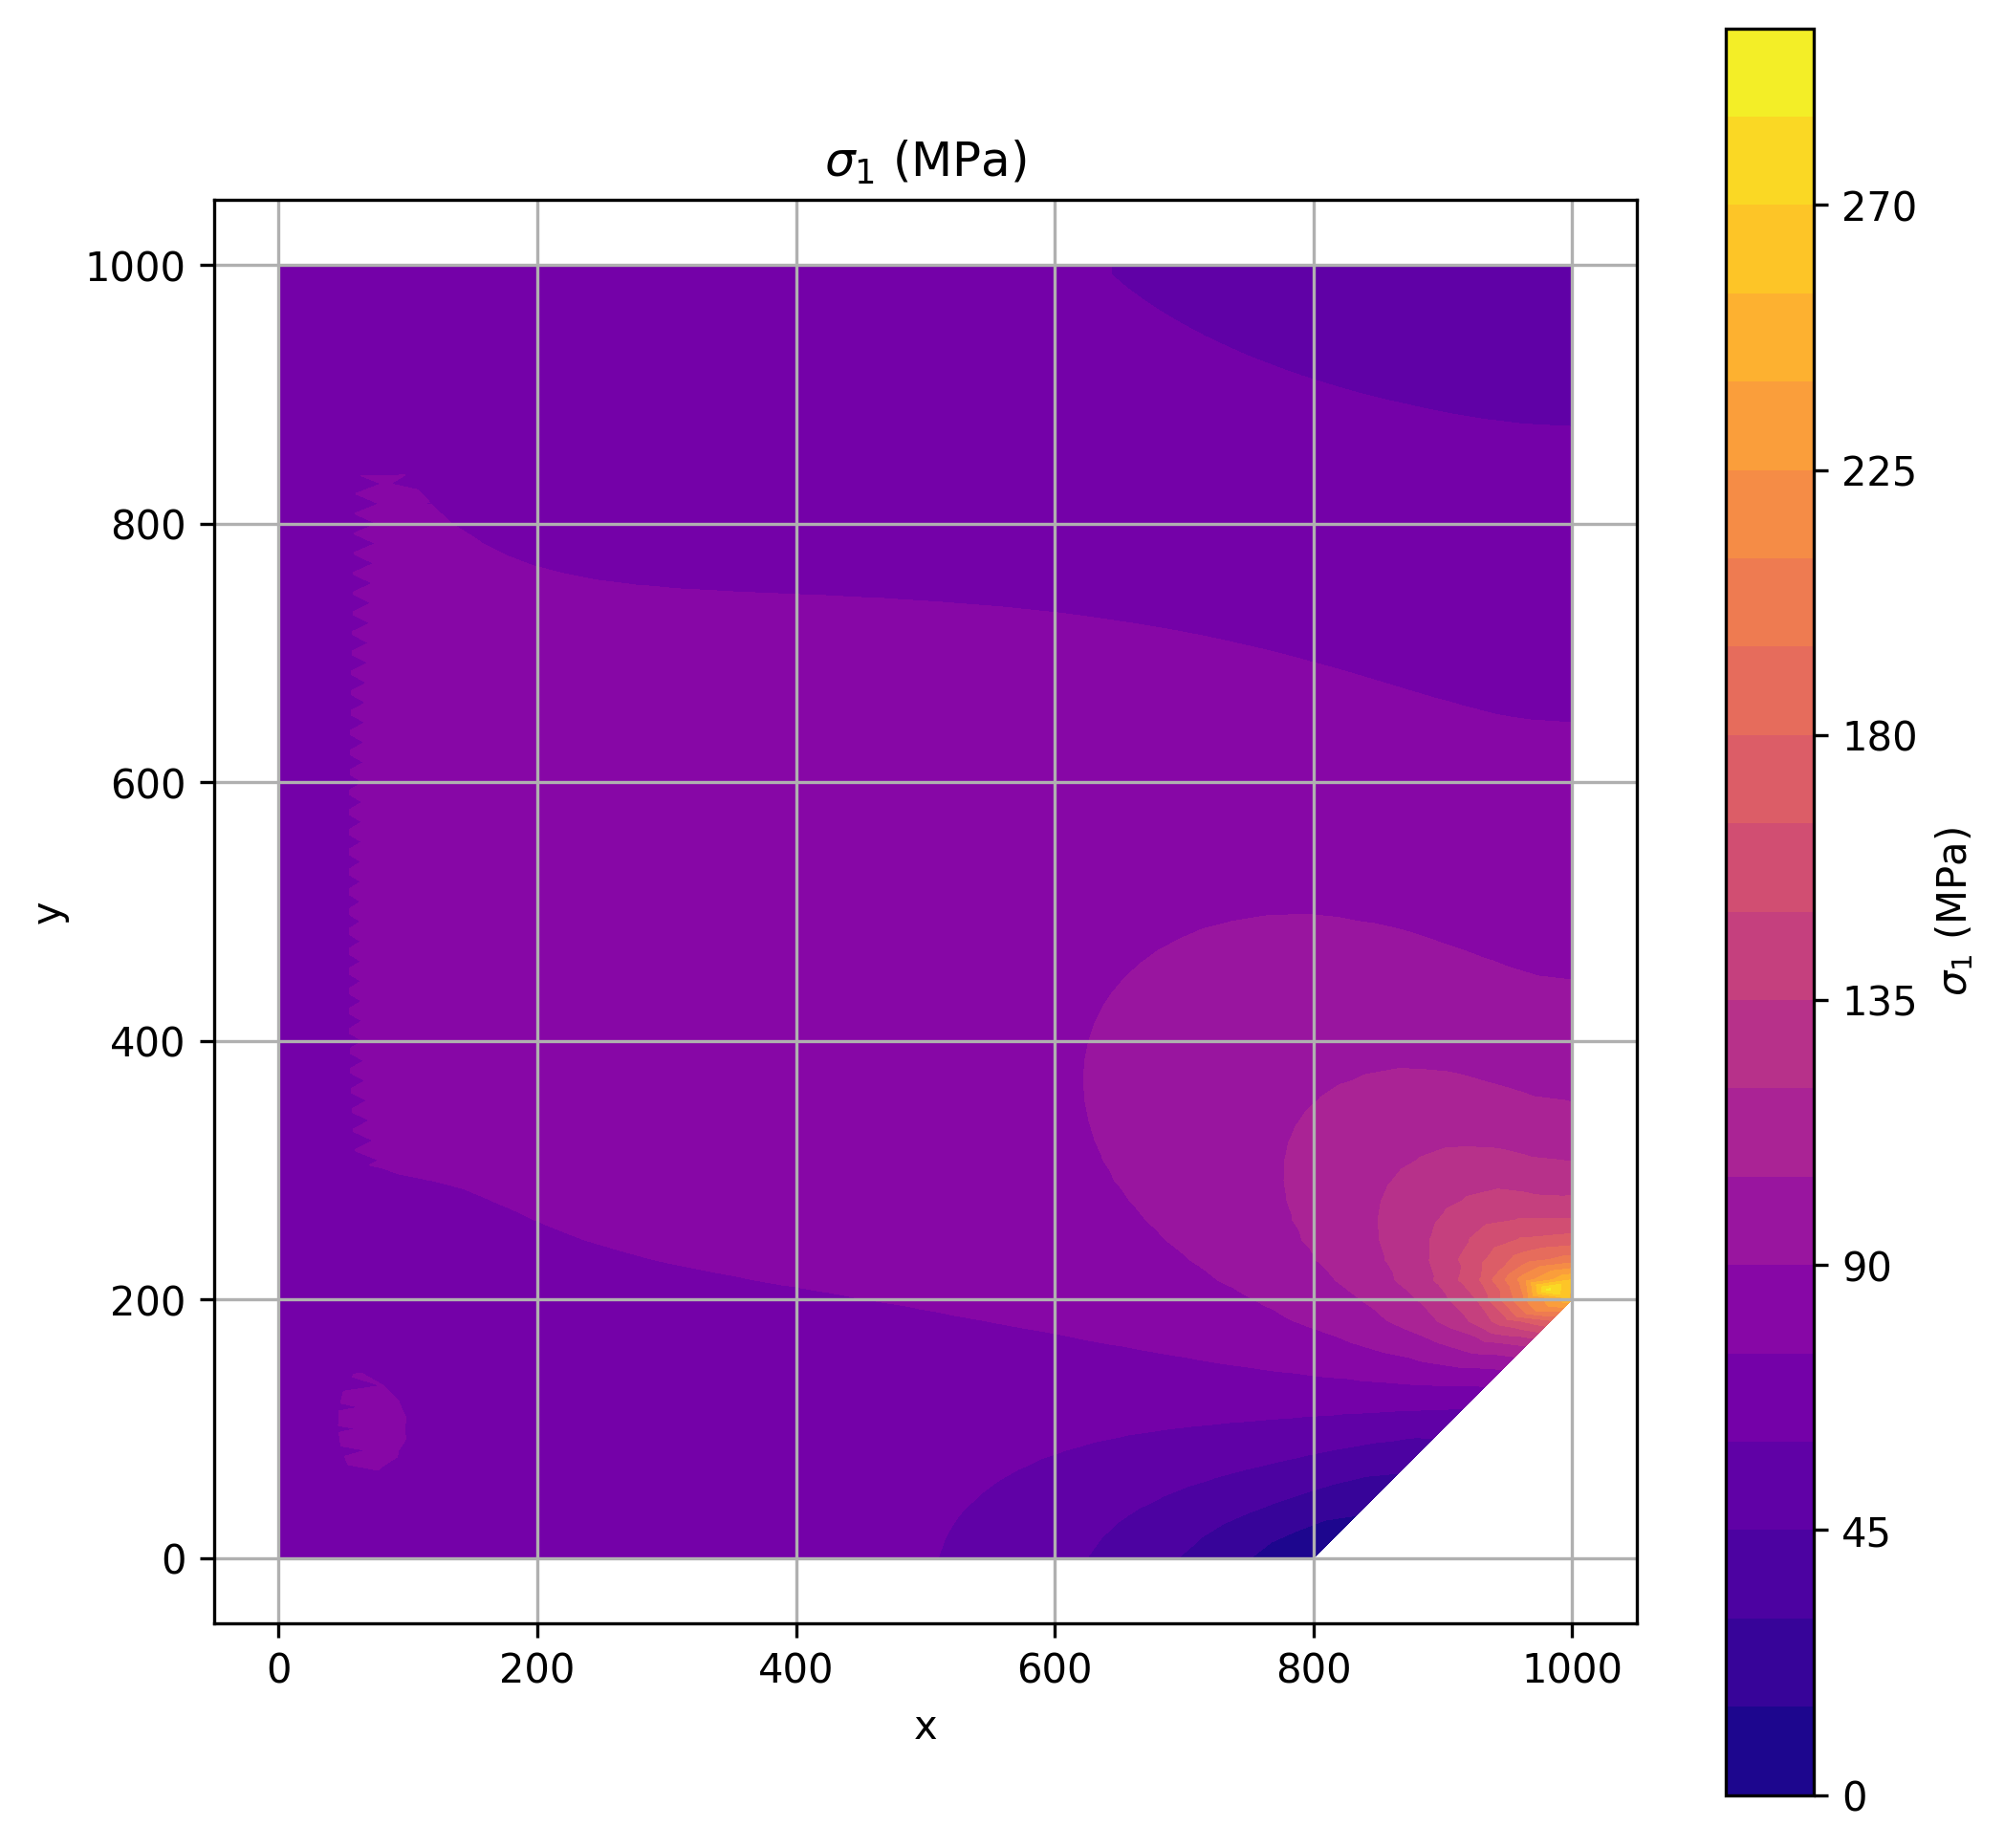
\includegraphics[width=\textwidth]{GRAFICOS/Quad9/1.75mm_global/resultados - sigma_1.png}
    \caption{Global mesh refinement - $h=1.75mm$}
    \label{fig:img11}
  \end{subfigure}
  \hfill
  \begin{subfigure}[b]{0.45\textwidth}
    \centering
    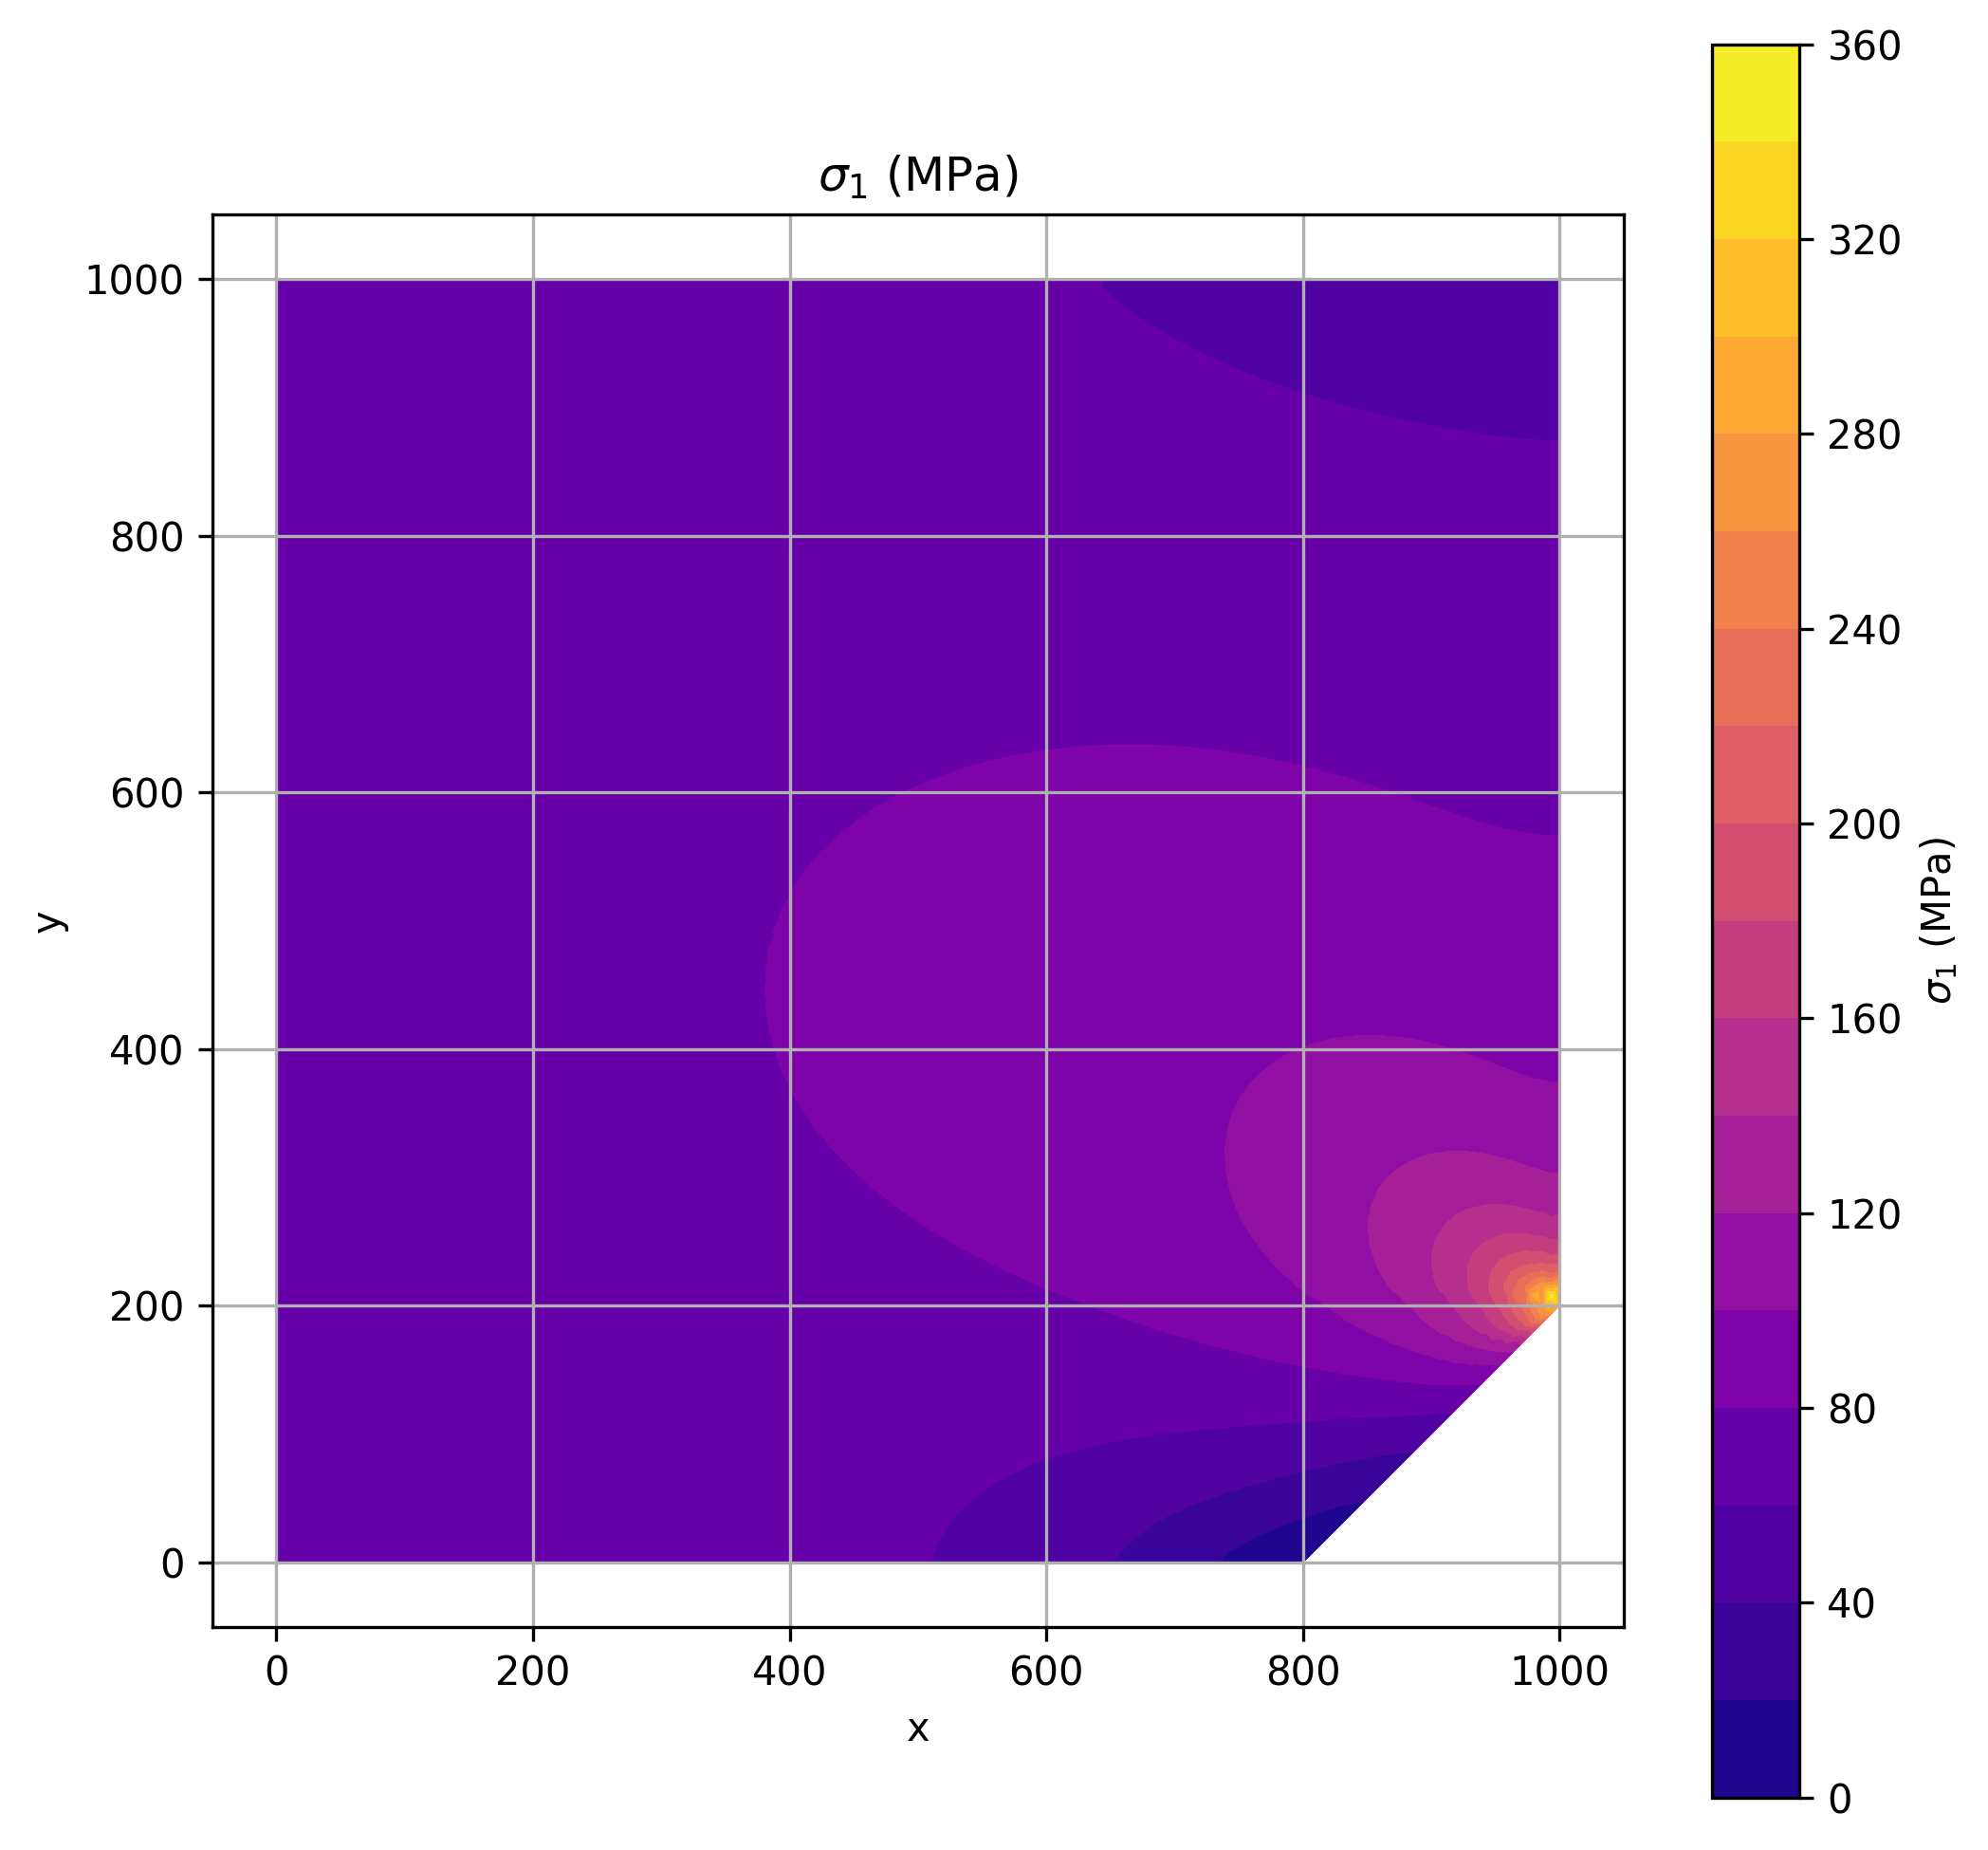
\includegraphics[width=\textwidth]{GRAFICOS/Quad9/1.75mm_local/resultados - sigma_1.png}
    \caption{Local mesh refinement - $h=1.75mm$}
    \label{fig:img21}
  \end{subfigure}
\end{figure}

\begin{figure}[H]
  \centering
  \begin{subfigure}[b]{0.45\textwidth}
    \centering
    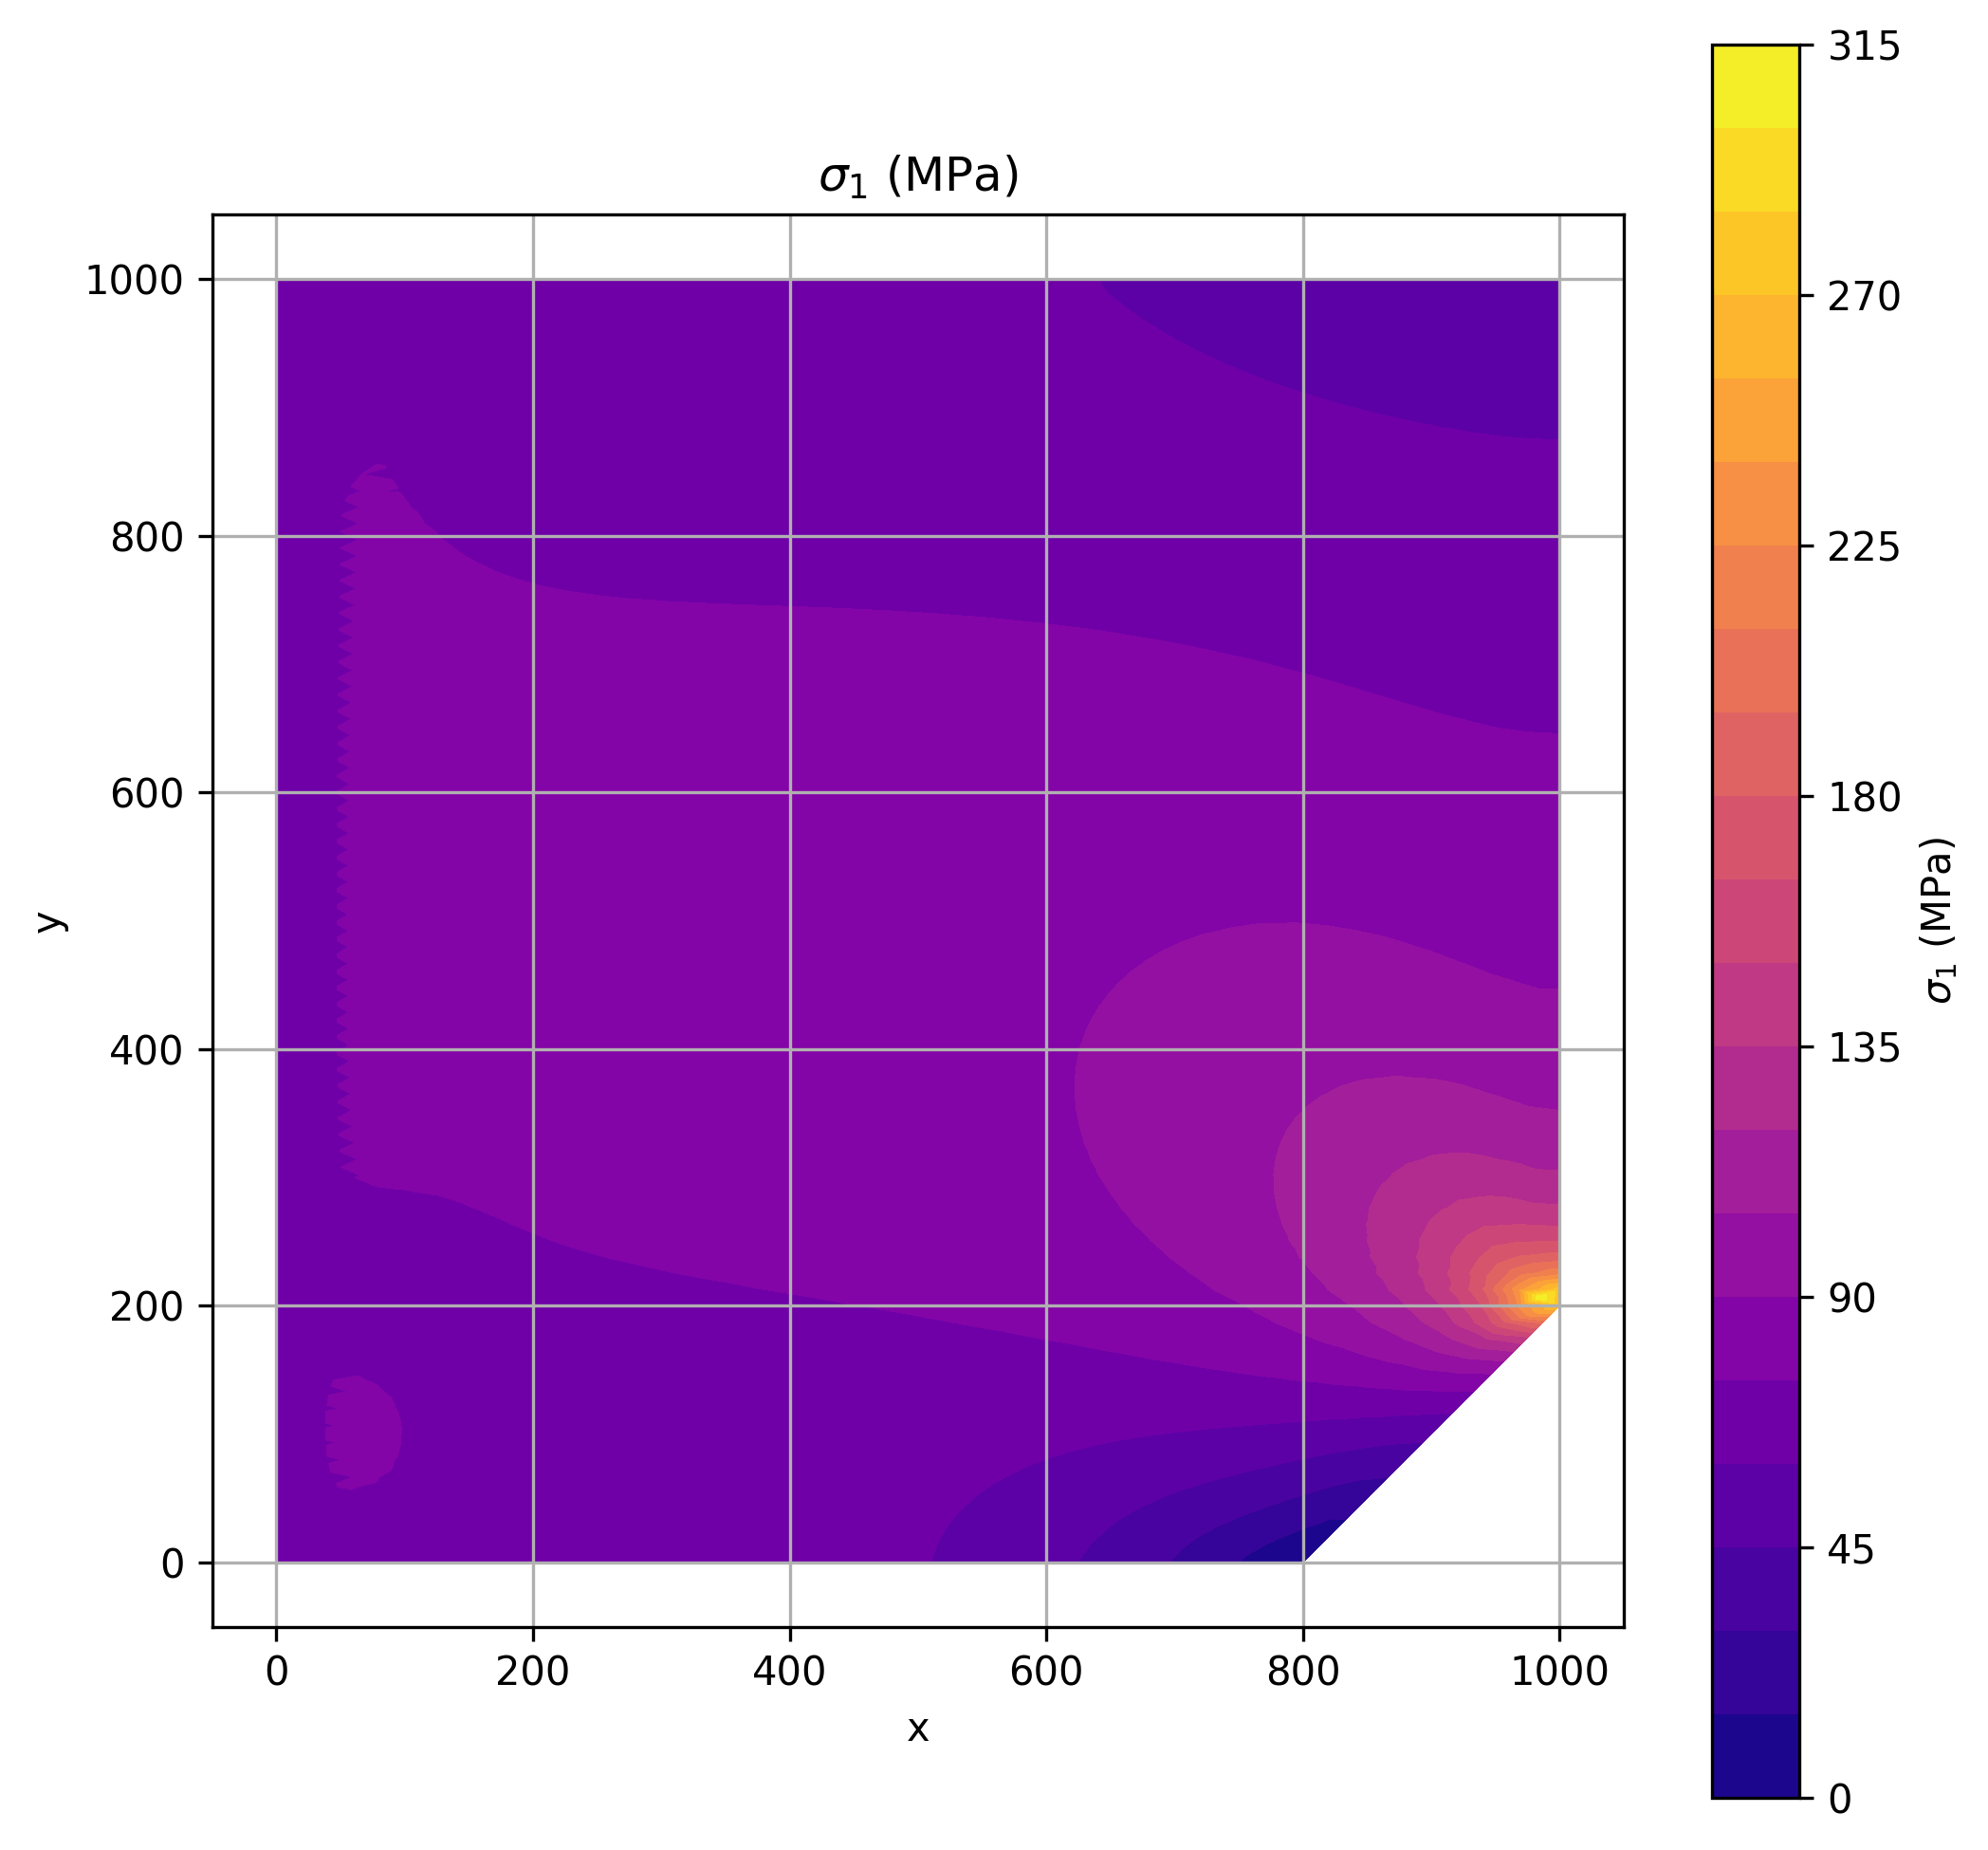
\includegraphics[width=\textwidth]{GRAFICOS/Quad9/1.5mm_global/resultados - sigma_1.png}
    \caption{Global mesh refinement - $h=1.5mm$}
    \label{fig:img12}
  \end{subfigure}
  \hfill
  \begin{subfigure}[b]{0.45\textwidth}
    \centering
    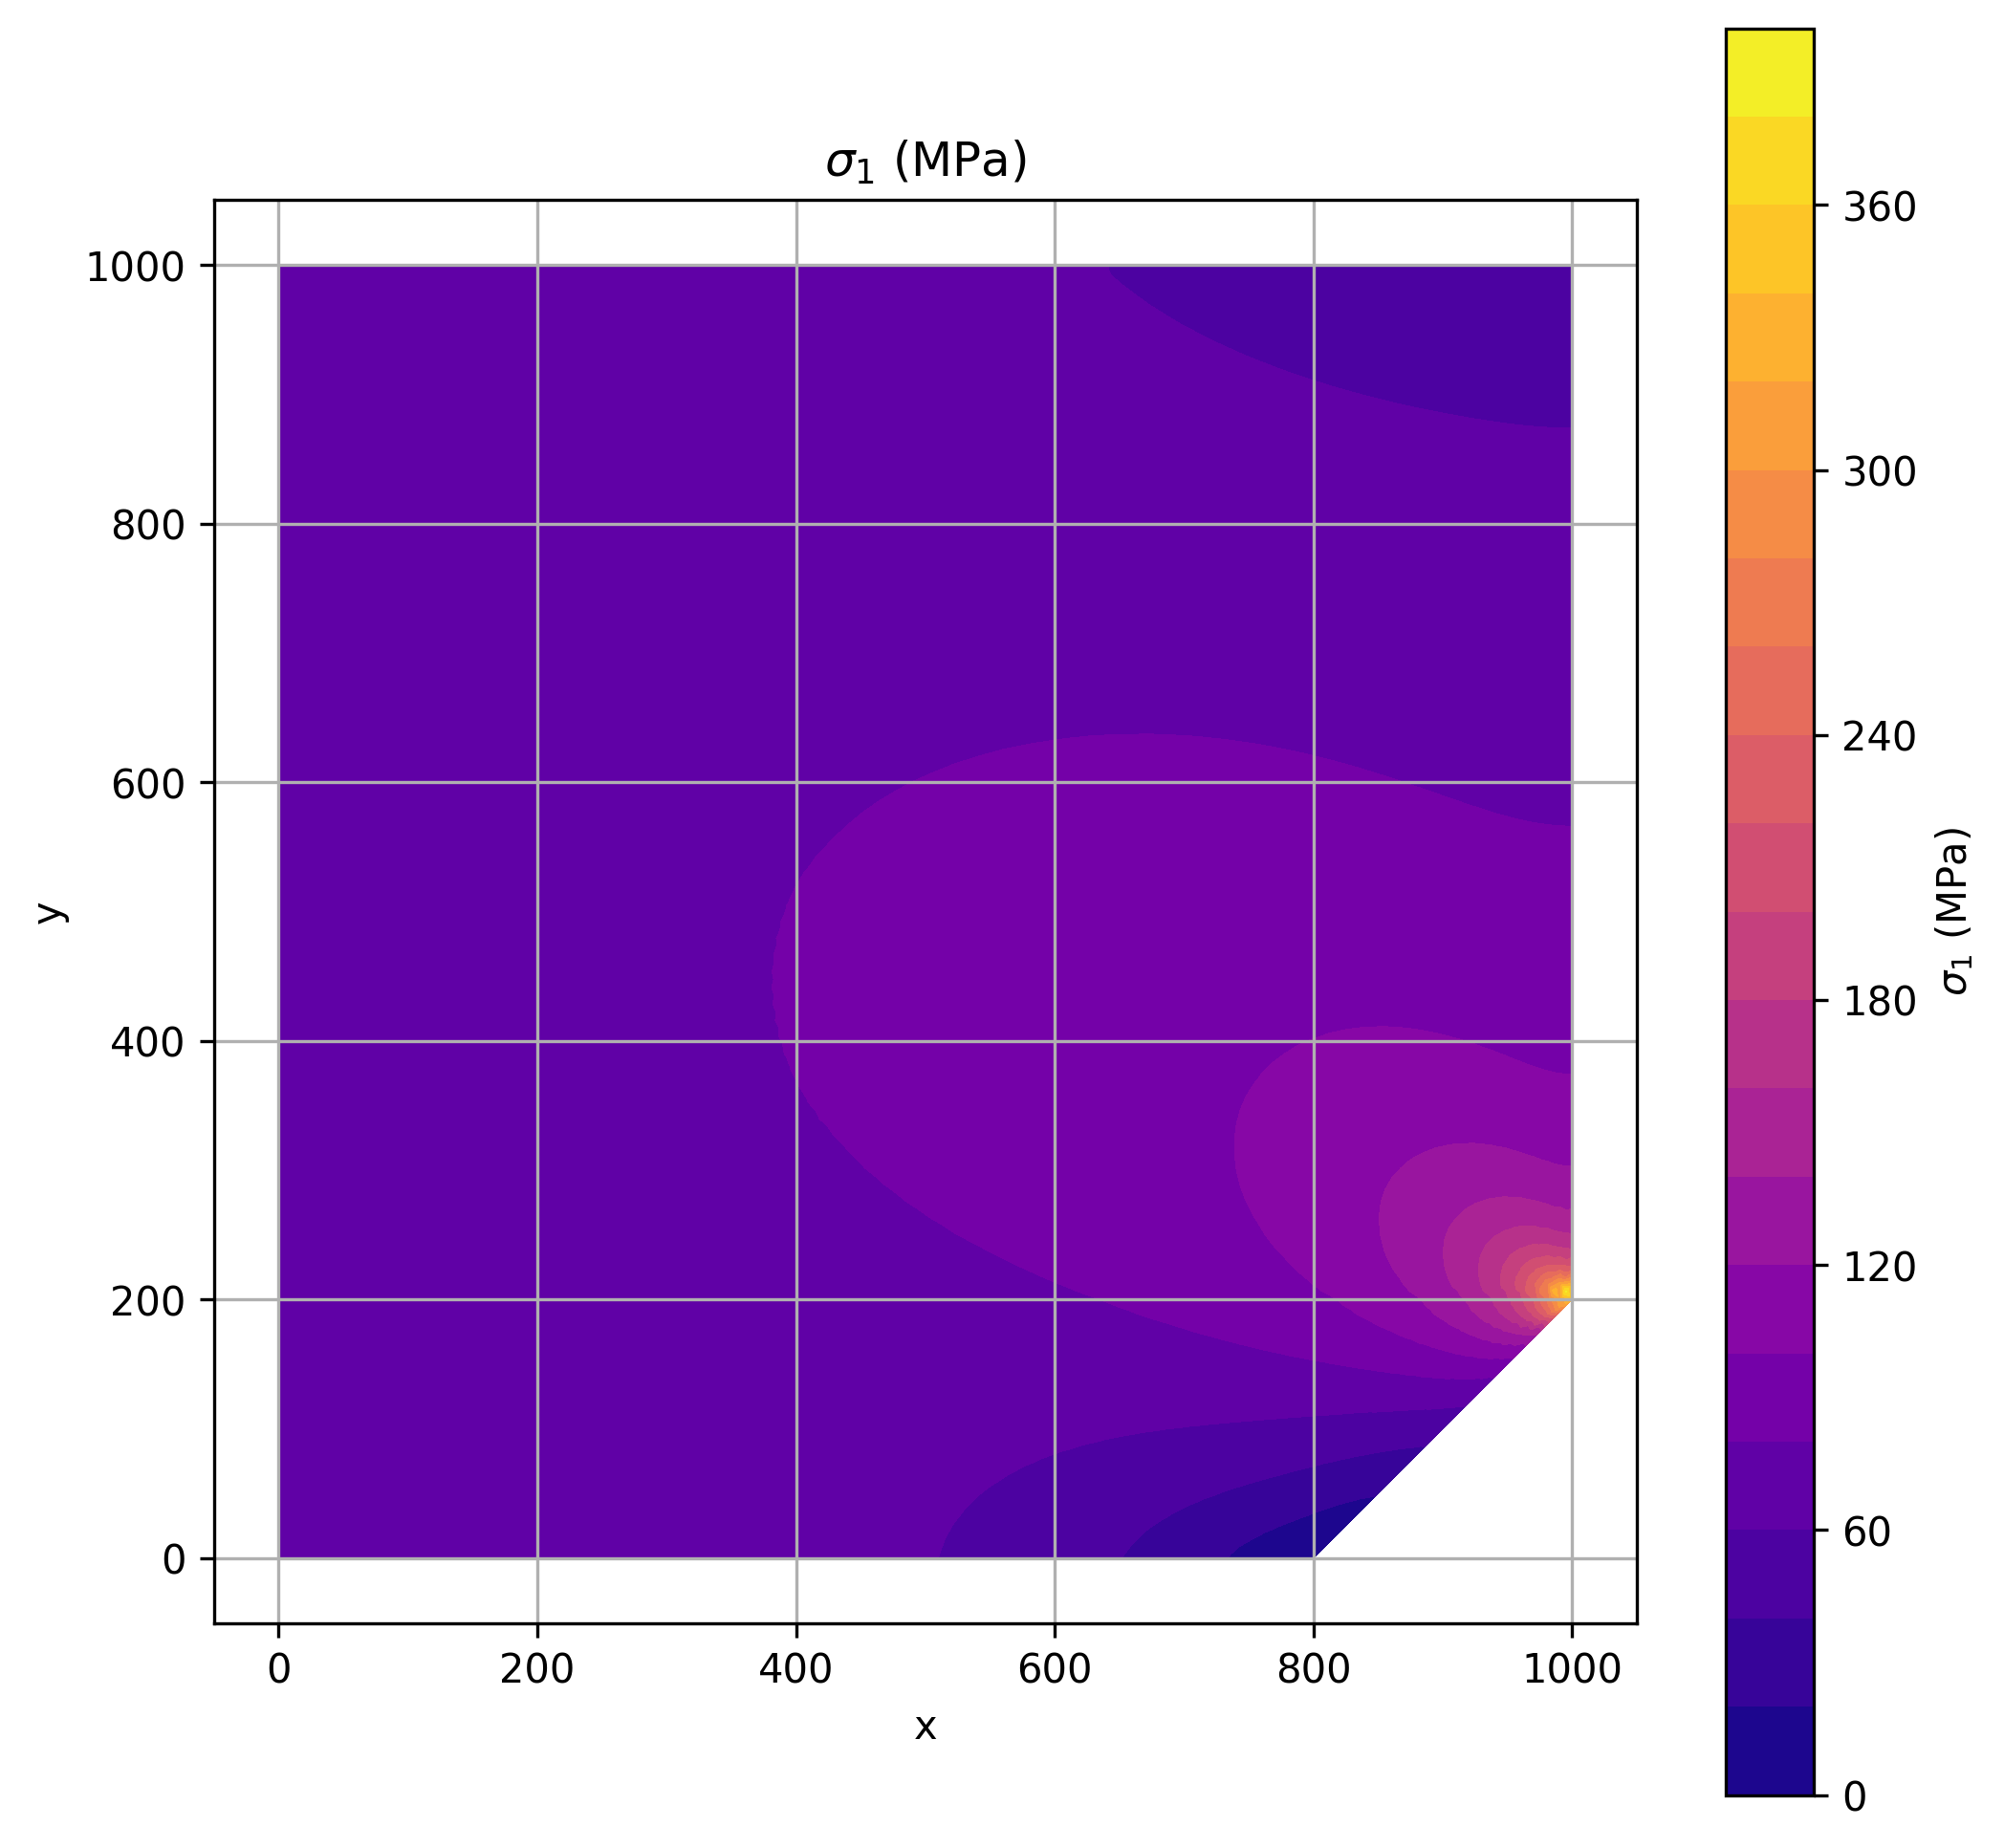
\includegraphics[width=\textwidth]{GRAFICOS/Quad9/1.5mm_local/resultados - sigma_1.png}
    \caption{Local mesh refinement - $h=1.5mm$}
    \label{fig:img22}
  \end{subfigure}
\end{figure}

\begin{figure}[H]
  \centering
  \begin{subfigure}[b]{0.45\textwidth}
    \centering
    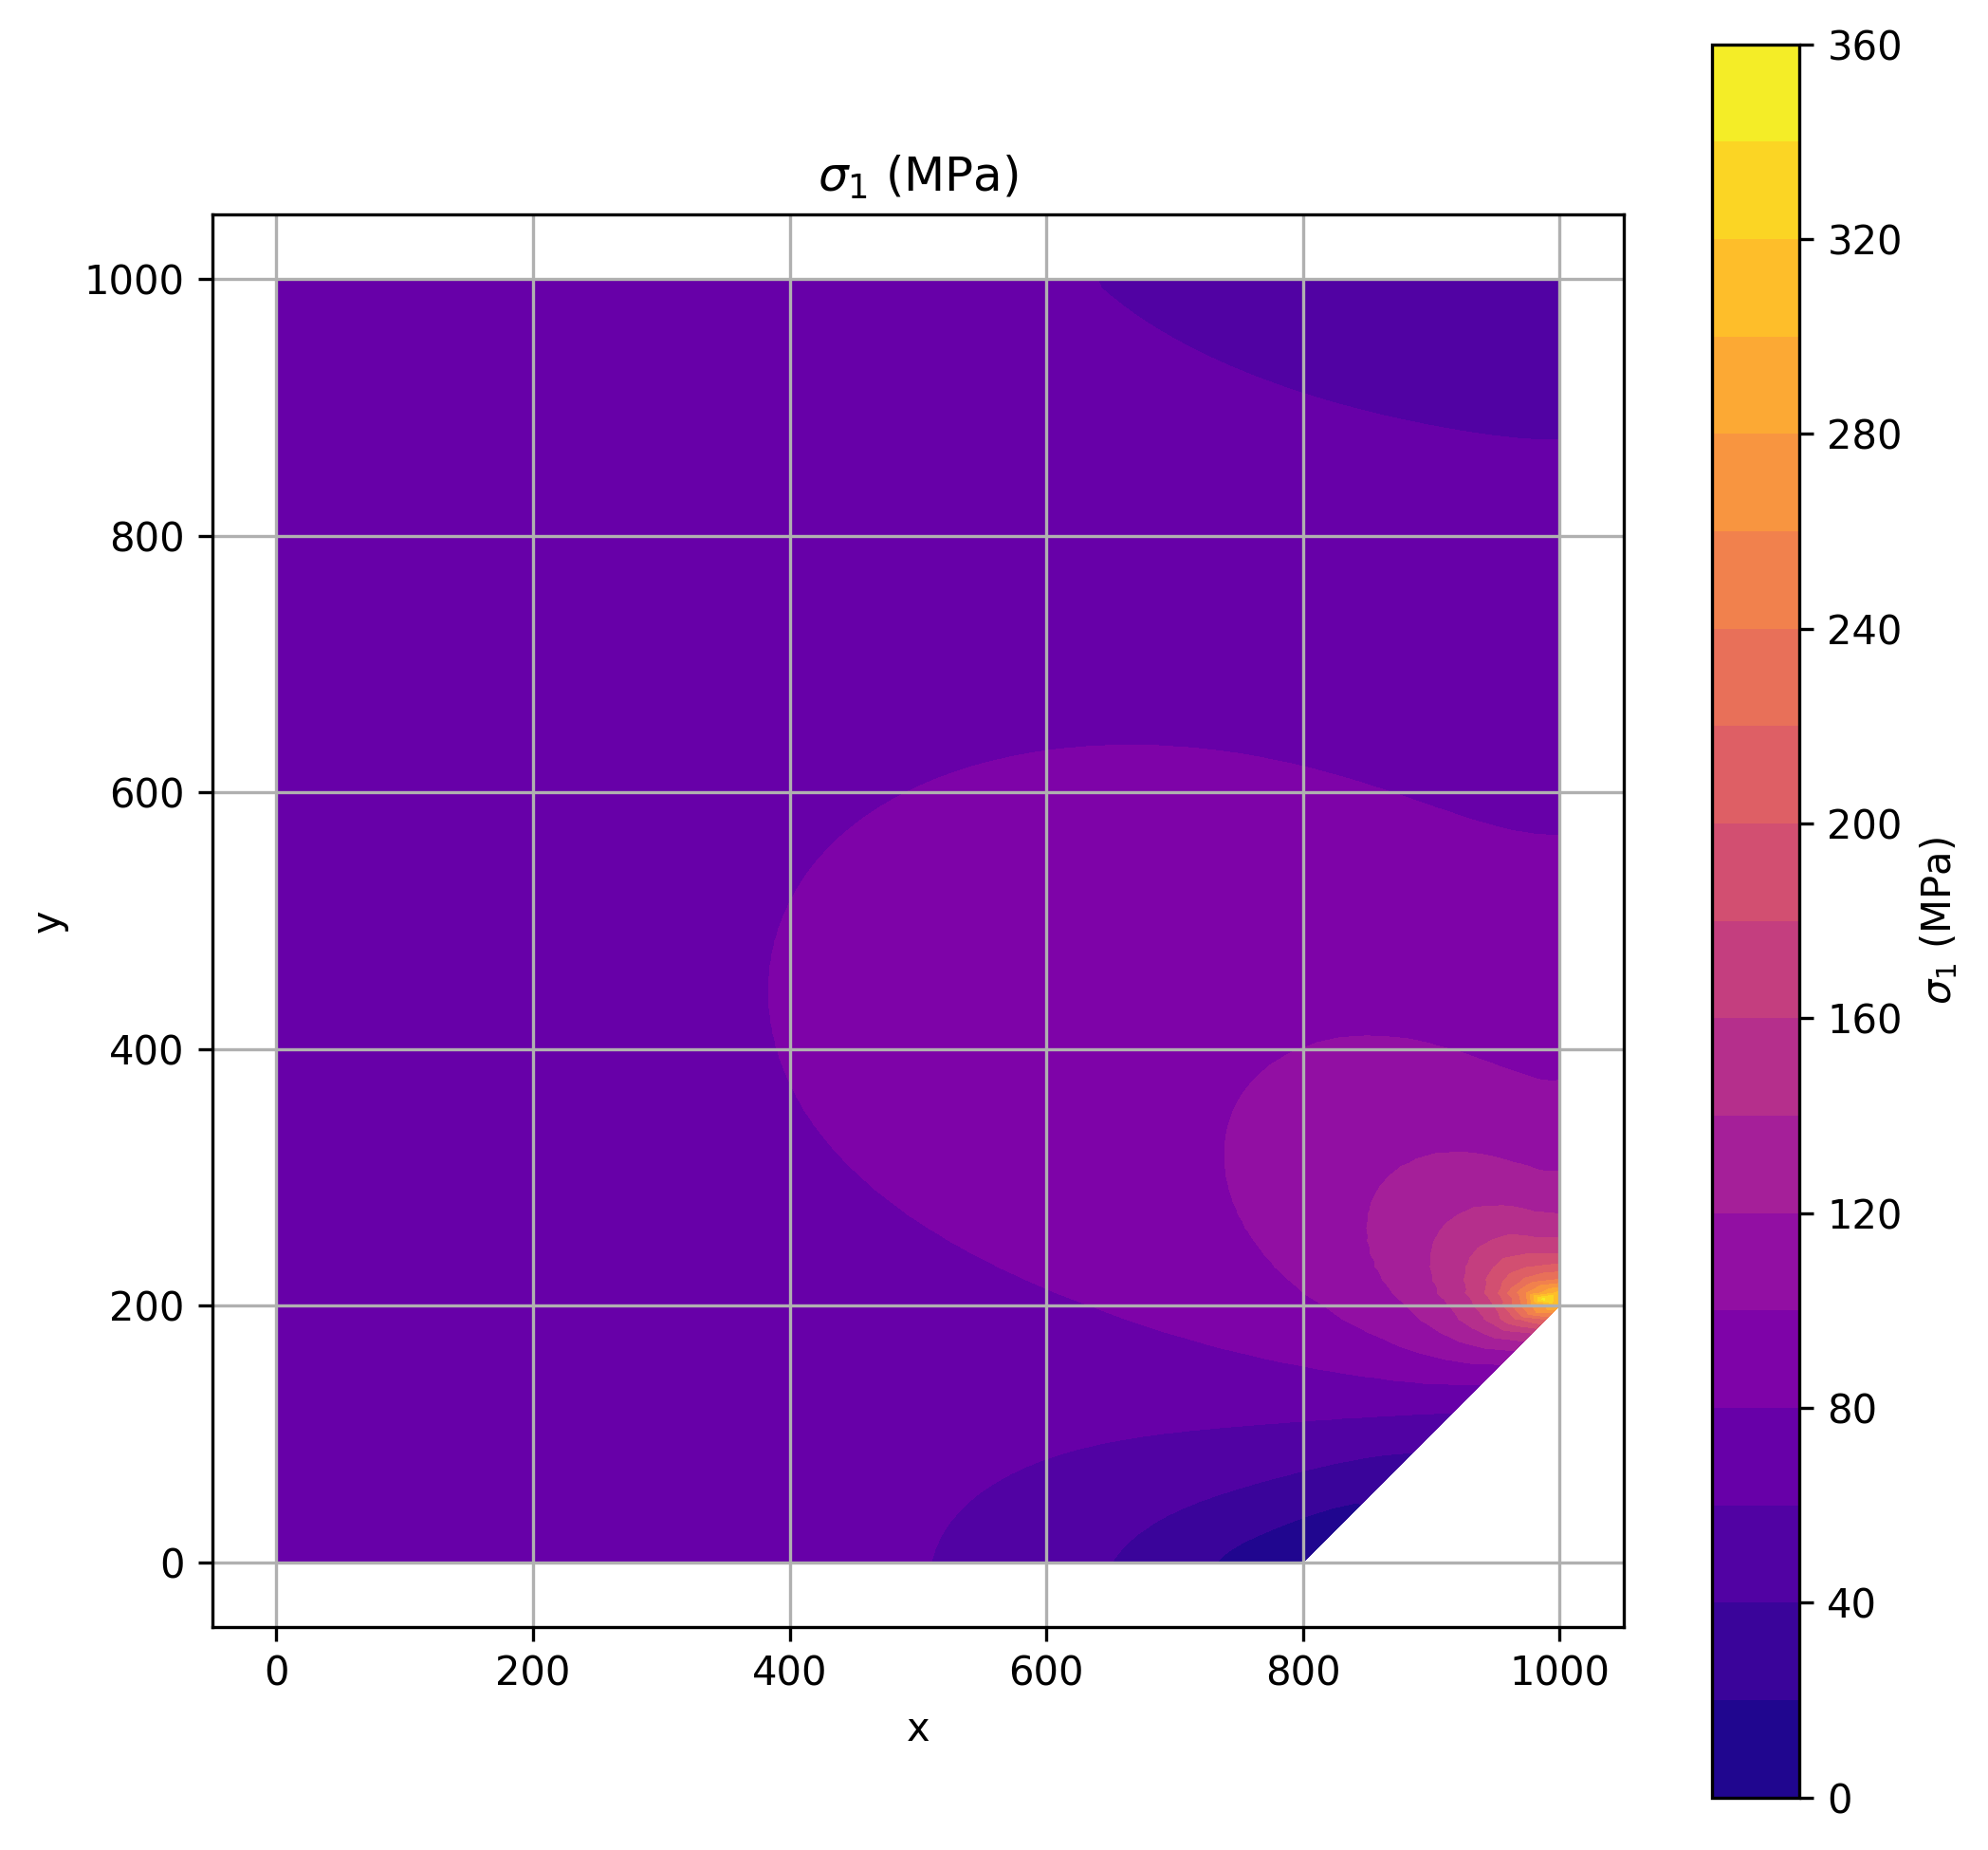
\includegraphics[width=\textwidth]{GRAFICOS/Quad9/1.25mm_global/resultados - sigma_1.png}
    \caption{Global mesh refinement - $h=1.25mm$}
    \label{fig:img13}
  \end{subfigure}
  \hfill
  \begin{subfigure}[b]{0.45\textwidth}
    \centering
    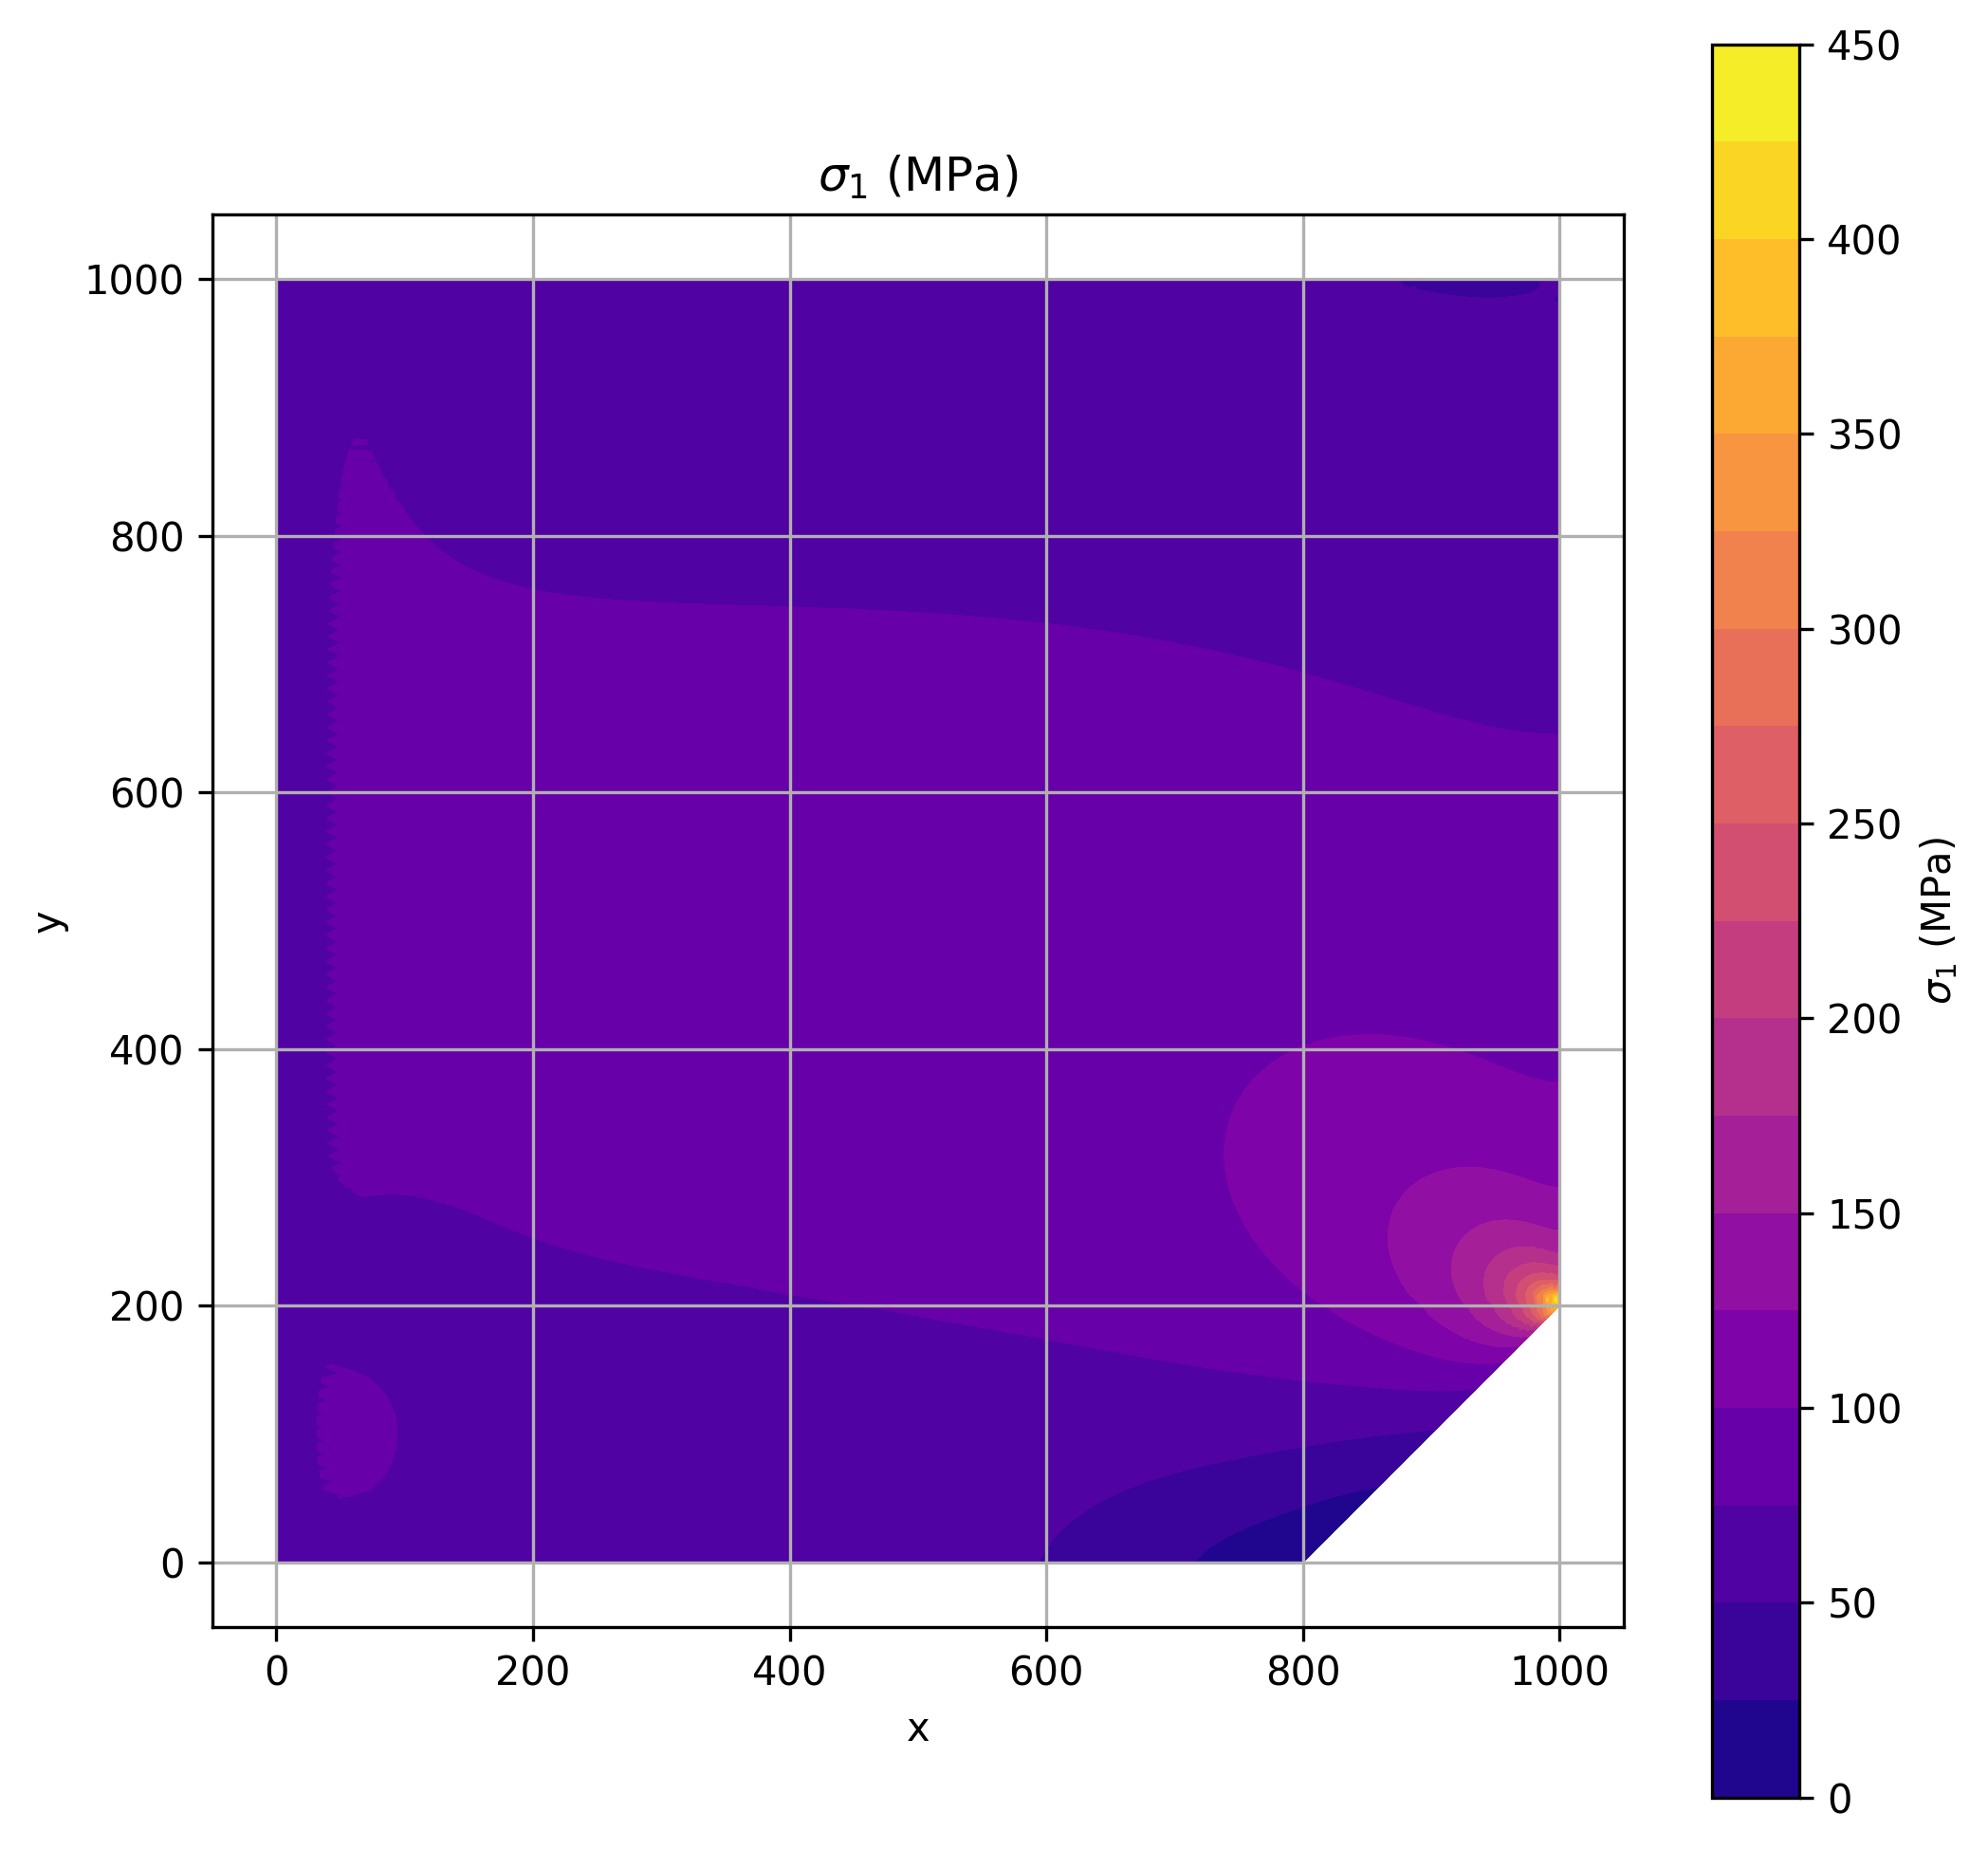
\includegraphics[width=\textwidth]{GRAFICOS/Quad9/1.25mm_local/resultados - sigma_1.png}
    \caption{Local mesh refinement - $h=1.25mm$}
    \label{fig:img23}
  \end{subfigure}
\end{figure}

\begin{table}[H]
  \centering
\caption{Table of $\sigma_{\max}$ with global and local refinement for different $h$ - Quad9 Elements}
  \begin{tabular}{|c|c|c|}
    \hline
    \multicolumn{3}{|c|}{$\sigma_{max} (MPa)$} \\ \hline
    $h$ (mm) & Global & Local \\ \hline
    2 & 240.86 & 268.64 \\ \hline
    1.75 & 265.56 & 305.40 \\ \hline
    1.5 & 288.52 & 335.68 \\ \hline
    1.25 & 317.26 & 373.40 \\ \hline
  \end{tabular}
  \label{tab:12}
\end{table}

As it can be seen in the Tables \ref{tab:5x2} and \ref{tab:12}, the maximum stress increases as the mesh is refined, which is expected. However, the maximum stress is lower for Quad9 elements than for Quad4 elements in local refinment, which indicates that the higher order elements provide a more accurate representation of the stress distribution.

To do a complete stress analysis, the Von Misses stress was plotted for every mesh size and element type. They can be observed in the Apendix section. 

The codes for the stress plot can be found in the following links: \href{https://github.com/LukasWolff2002/TAREA_3_FINITE/blob/main/ENTREGA_2/QUAD4/graph.py}{Code for Quad4 Stress Plot} and \href{https://github.com/LukasWolff2002/TAREA_3_FINITE/blob/main/ENTREGA_2/QUAD9/graph.py}{Code for Quad9 Stress Plot}.

\subsection{Part c)}

In this section, an optimization of the strcutre was made. Moreover, it was modeled and simulated, resulting in a complete stress and behaviour analysis.

The main objective was to anulate the stress concentration sections, in order to reduce the maximum stress in the strcuture and compare it with the previous results.

As it was mentioned above, the thickness used for the general analysis was $t=20mm$. To optimize the structure response and reduce the stress concentrations zones, iterations were made in every single element varying its thickness from $1mm$ to $40mm$, and comparying the stresses in each case, mantaining the total mass constant. The result was a multiple thickness structure.

\begin{figure}[H]
    \centering
    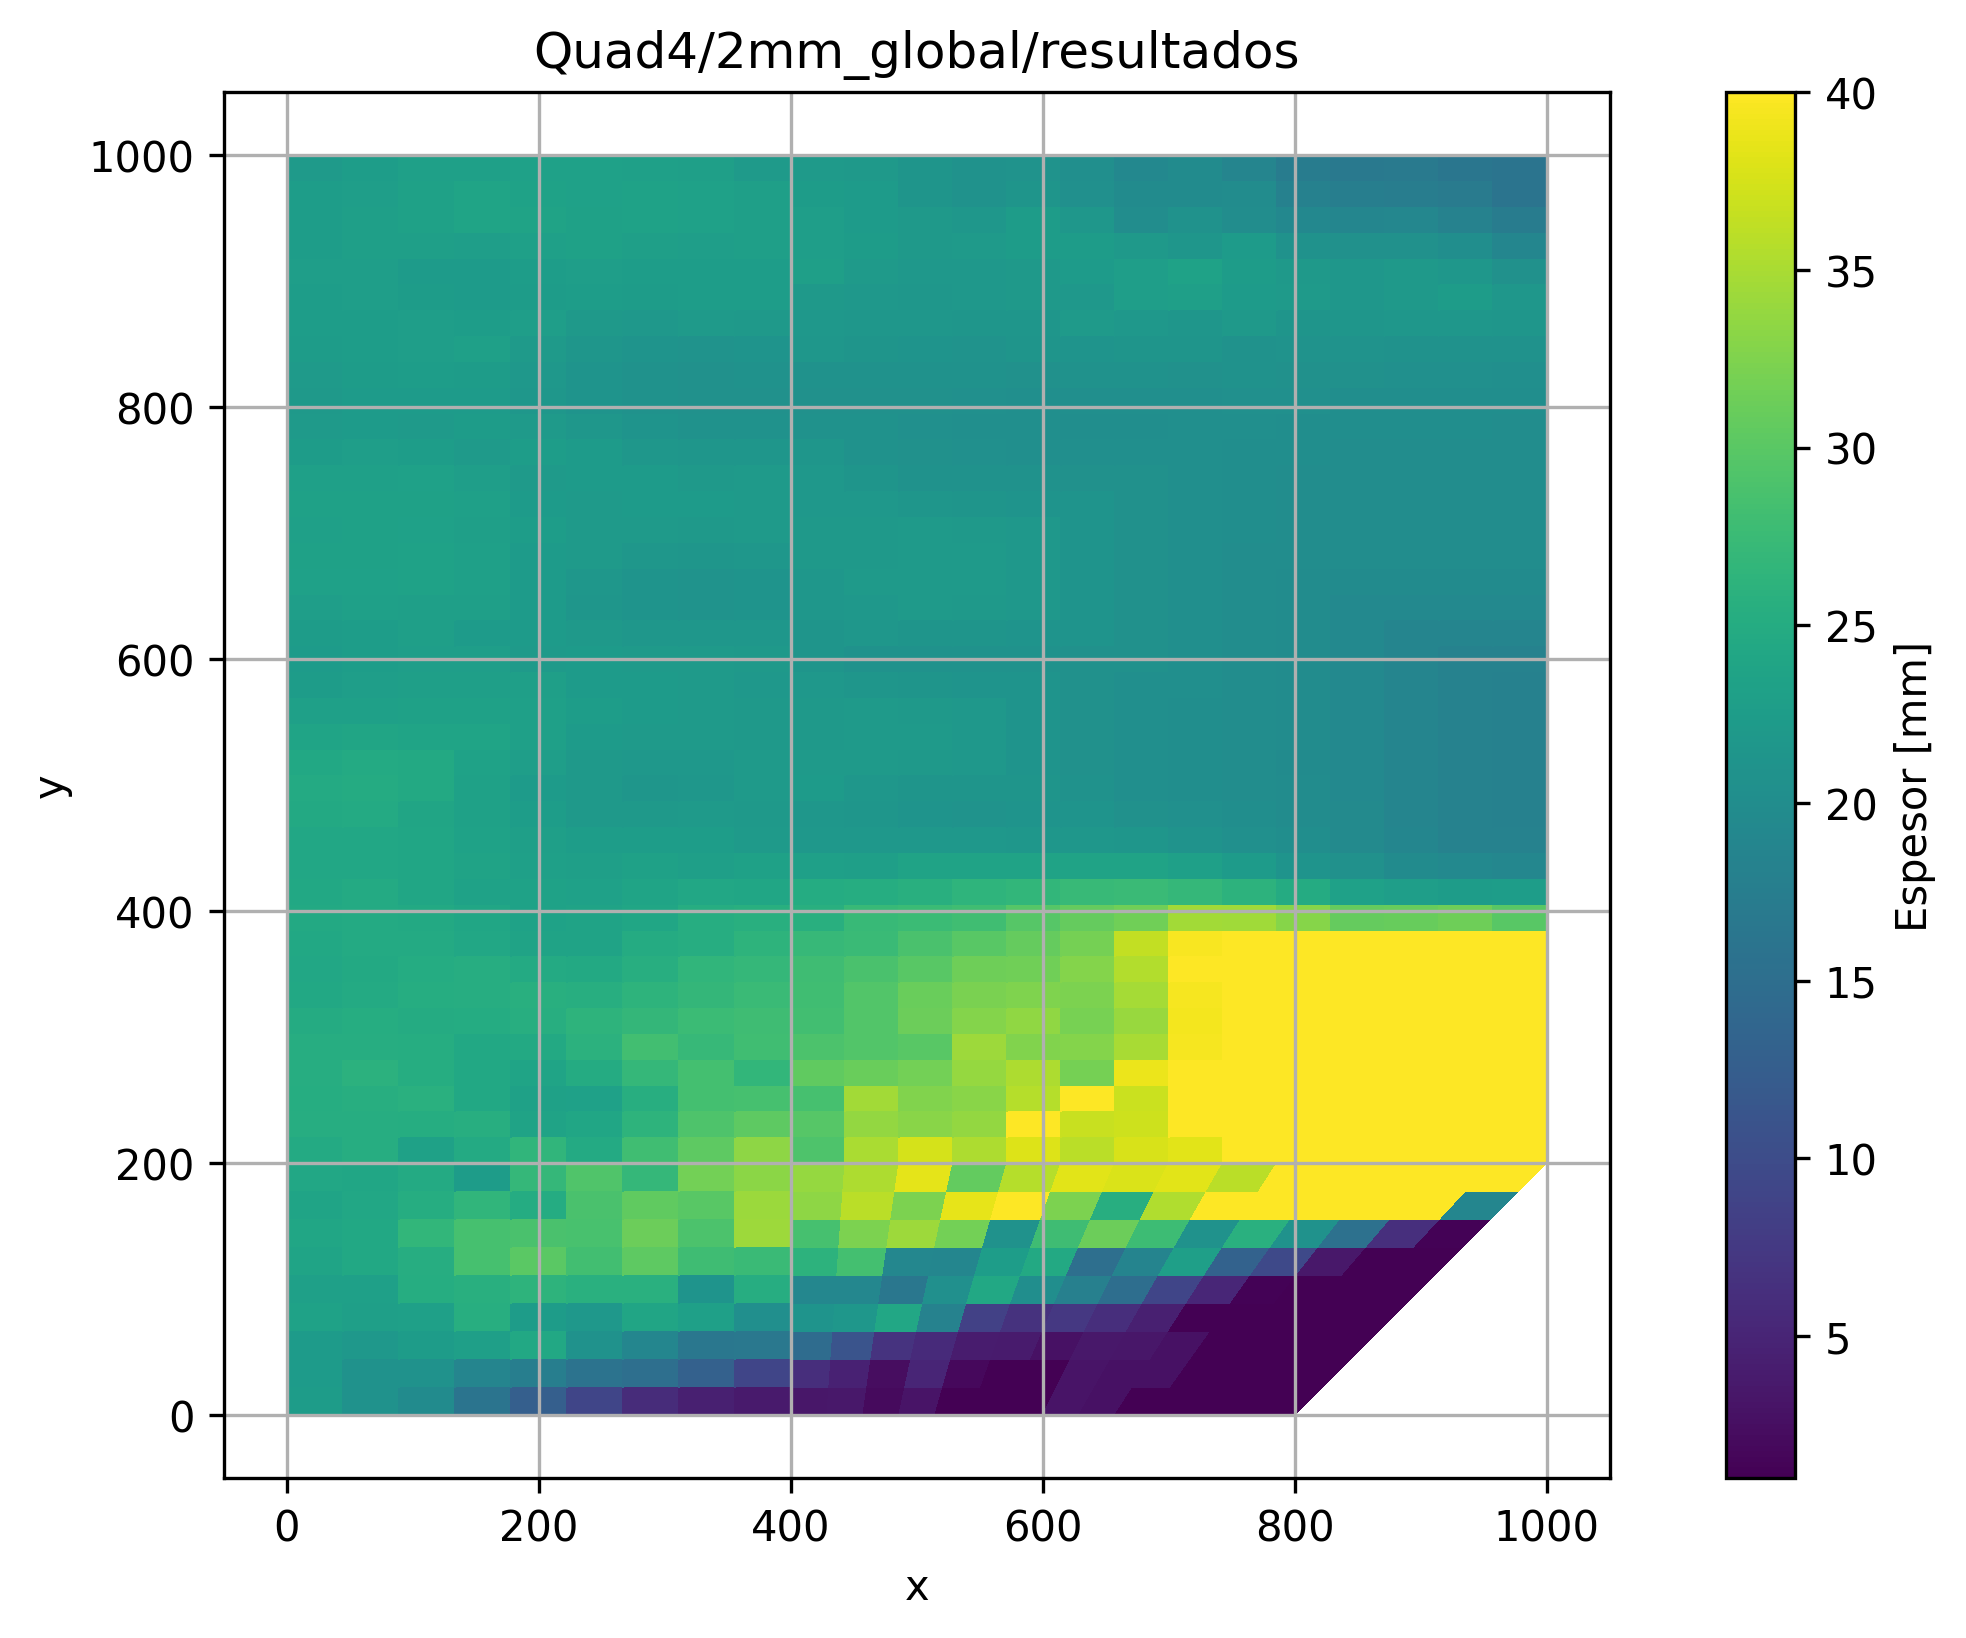
\includegraphics[width=0.5\textwidth]{GRAFICOS/Quad4/2mm_global/resultados_espesor_post_topologic.png}
    \caption{Optimized structure with multiple thicknesses}
    \label{fig:optimized_structure}
\end{figure}

With this result, the Von Misses stress distribution was modeled as follows.

\begin{figure}[H]
    \centering
    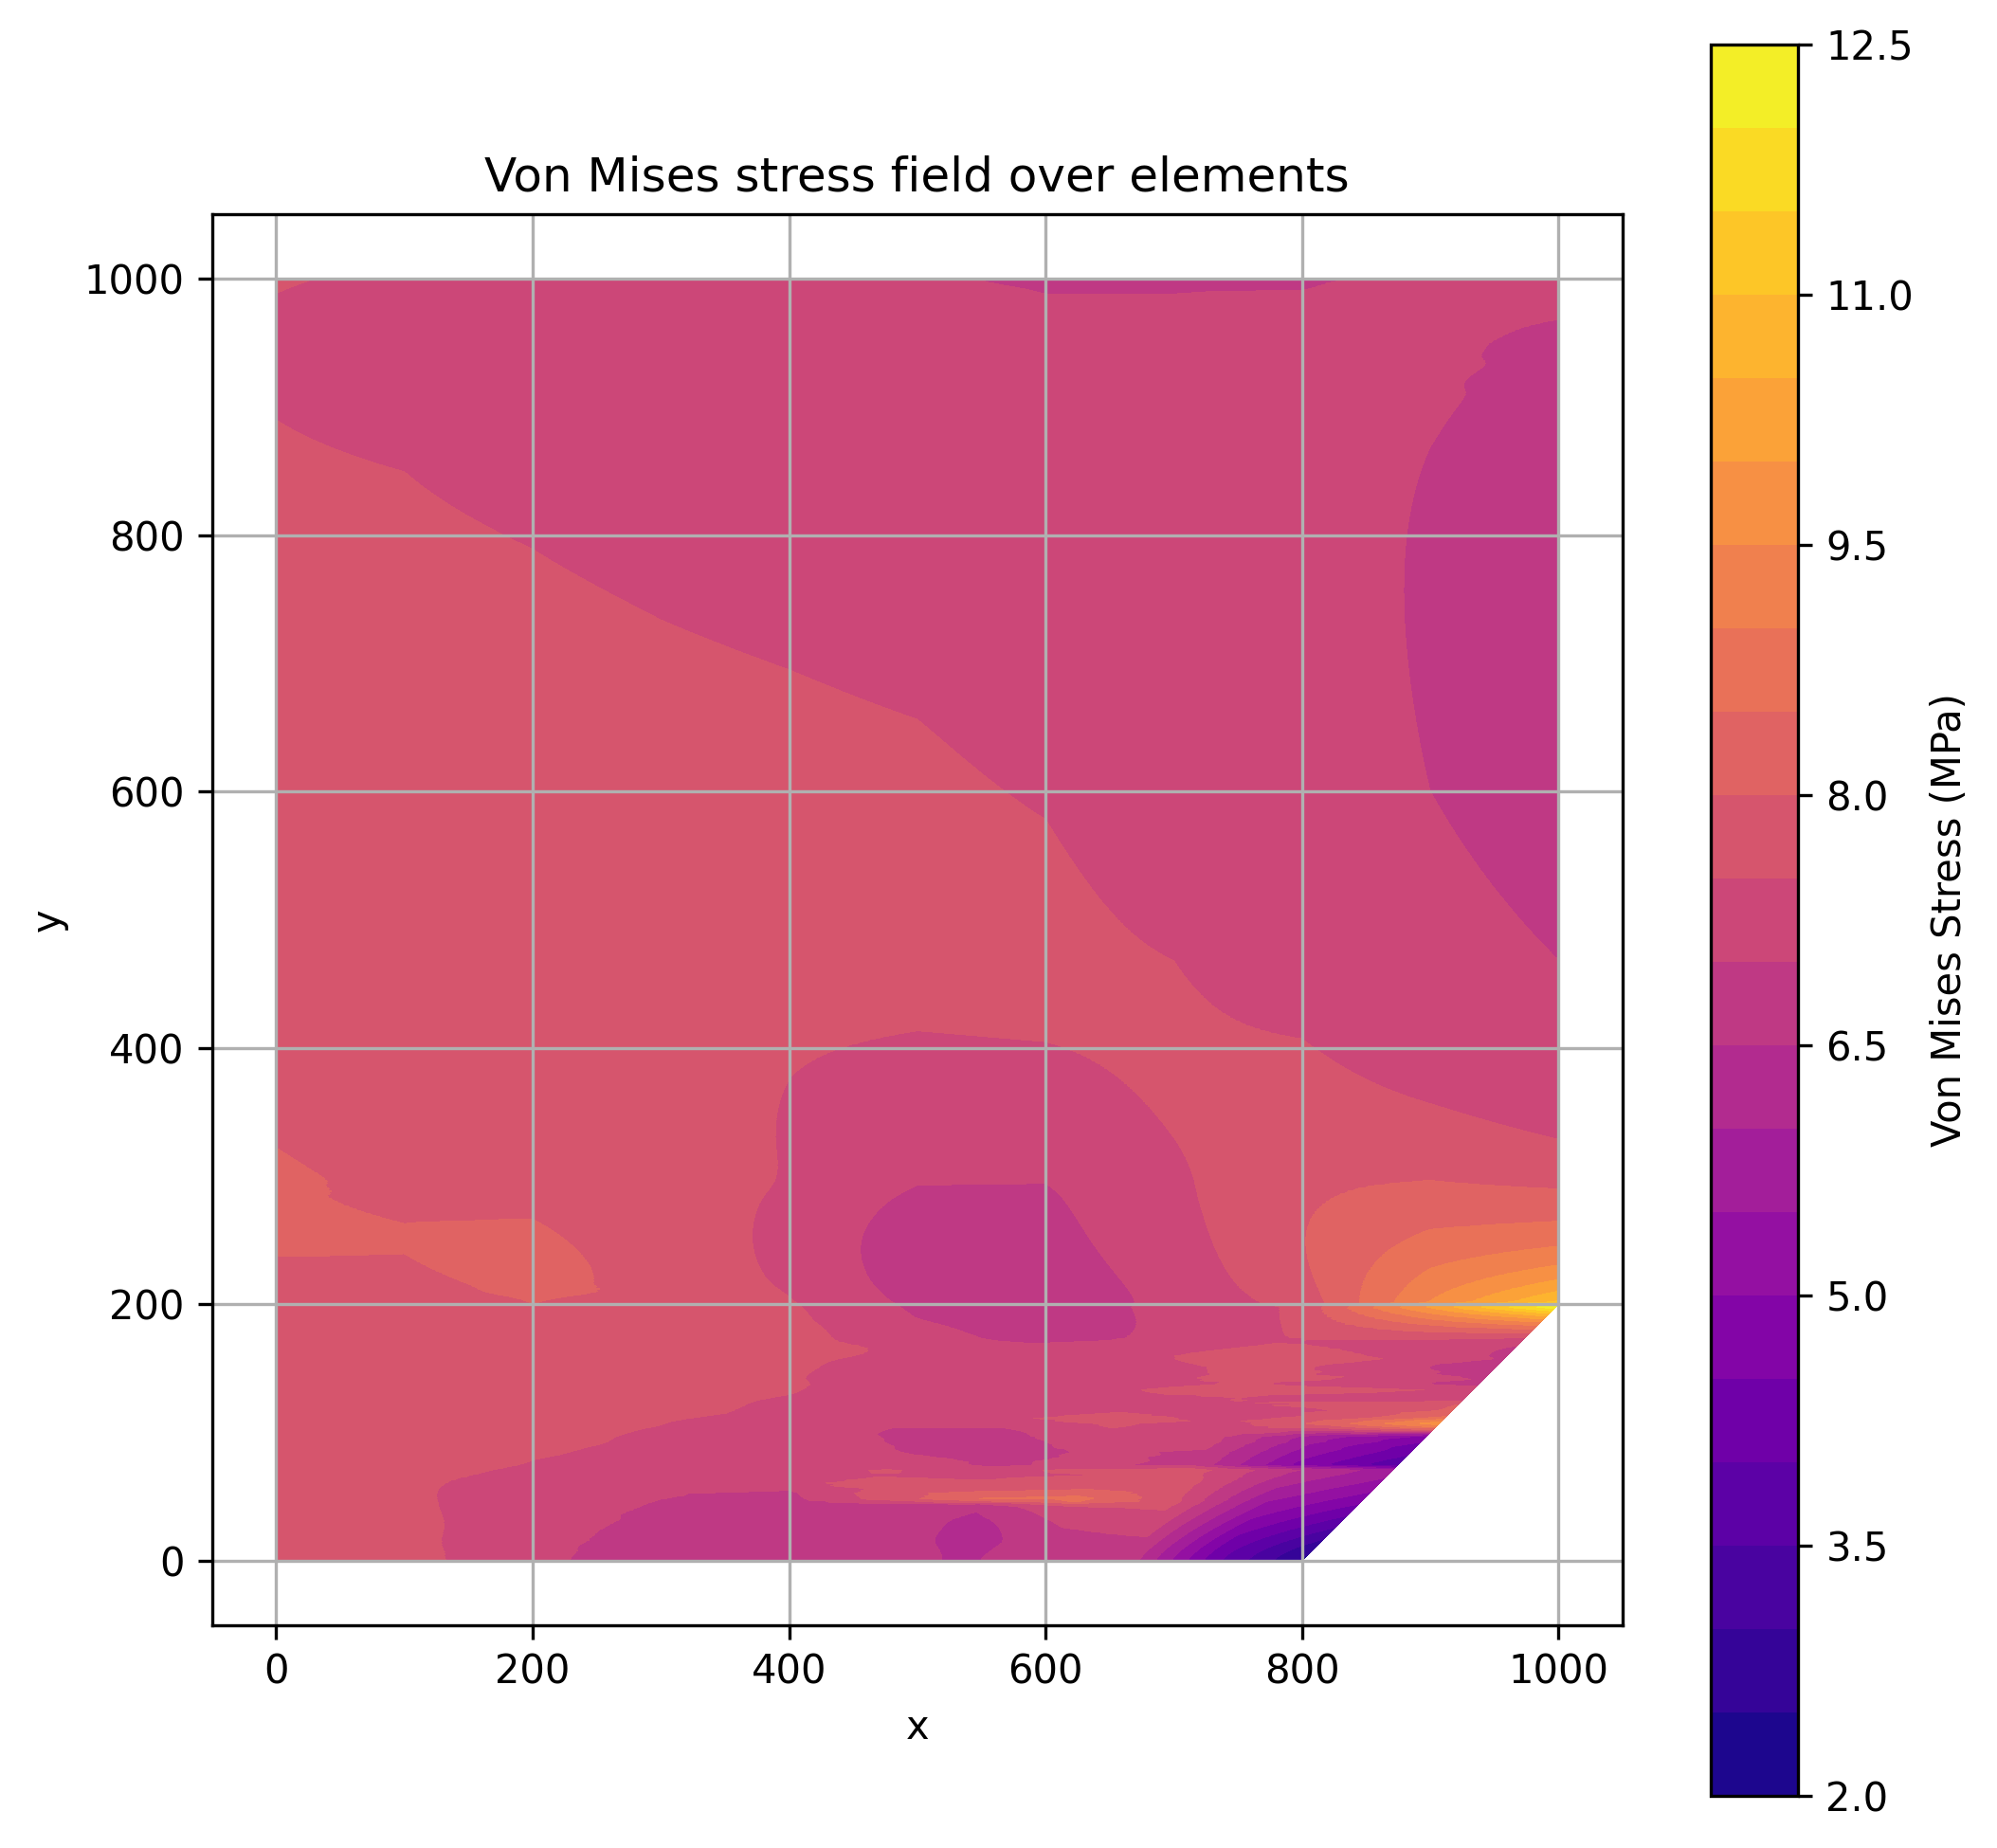
\includegraphics[width=0.5\textwidth]{GRAFICOS/Quad4/2mm_global/resultados_topo_von_mises_post_topologic.png}
    \caption{Von Misses stress distribution in the optimized structure}
    \label{fig:optimized_structure_stress}
\end{figure}

Figure \ref{fig:optimized_structure_stress} shows the Von Misses stress distribution in the optimized structure. As it can be seen, the maximum stress is $\sigma_{max} = 105 MPa$ which is significantly lower than the maximum stress in the previous analysis, taking into account all the mesh sizes.

Even though the stress concentration is not zero, an optimization in terms of decreasing the stress magnitud and mantaining the mass invariant was achieved. Making an overall stress distribution more homogeneous and uniform. This procedure is shown in the following code: \href{ https://github.com/LukasWolff2002/TAREA_3_FINITE/blob/main/ENTREGA_2/QUAD4/main.py}{Github code for Topological Optimization}.

The following graph, shows how the maximum principal stress converges with decreasing characteristic mesh size.

\begin{figure}[H]
    \centering
    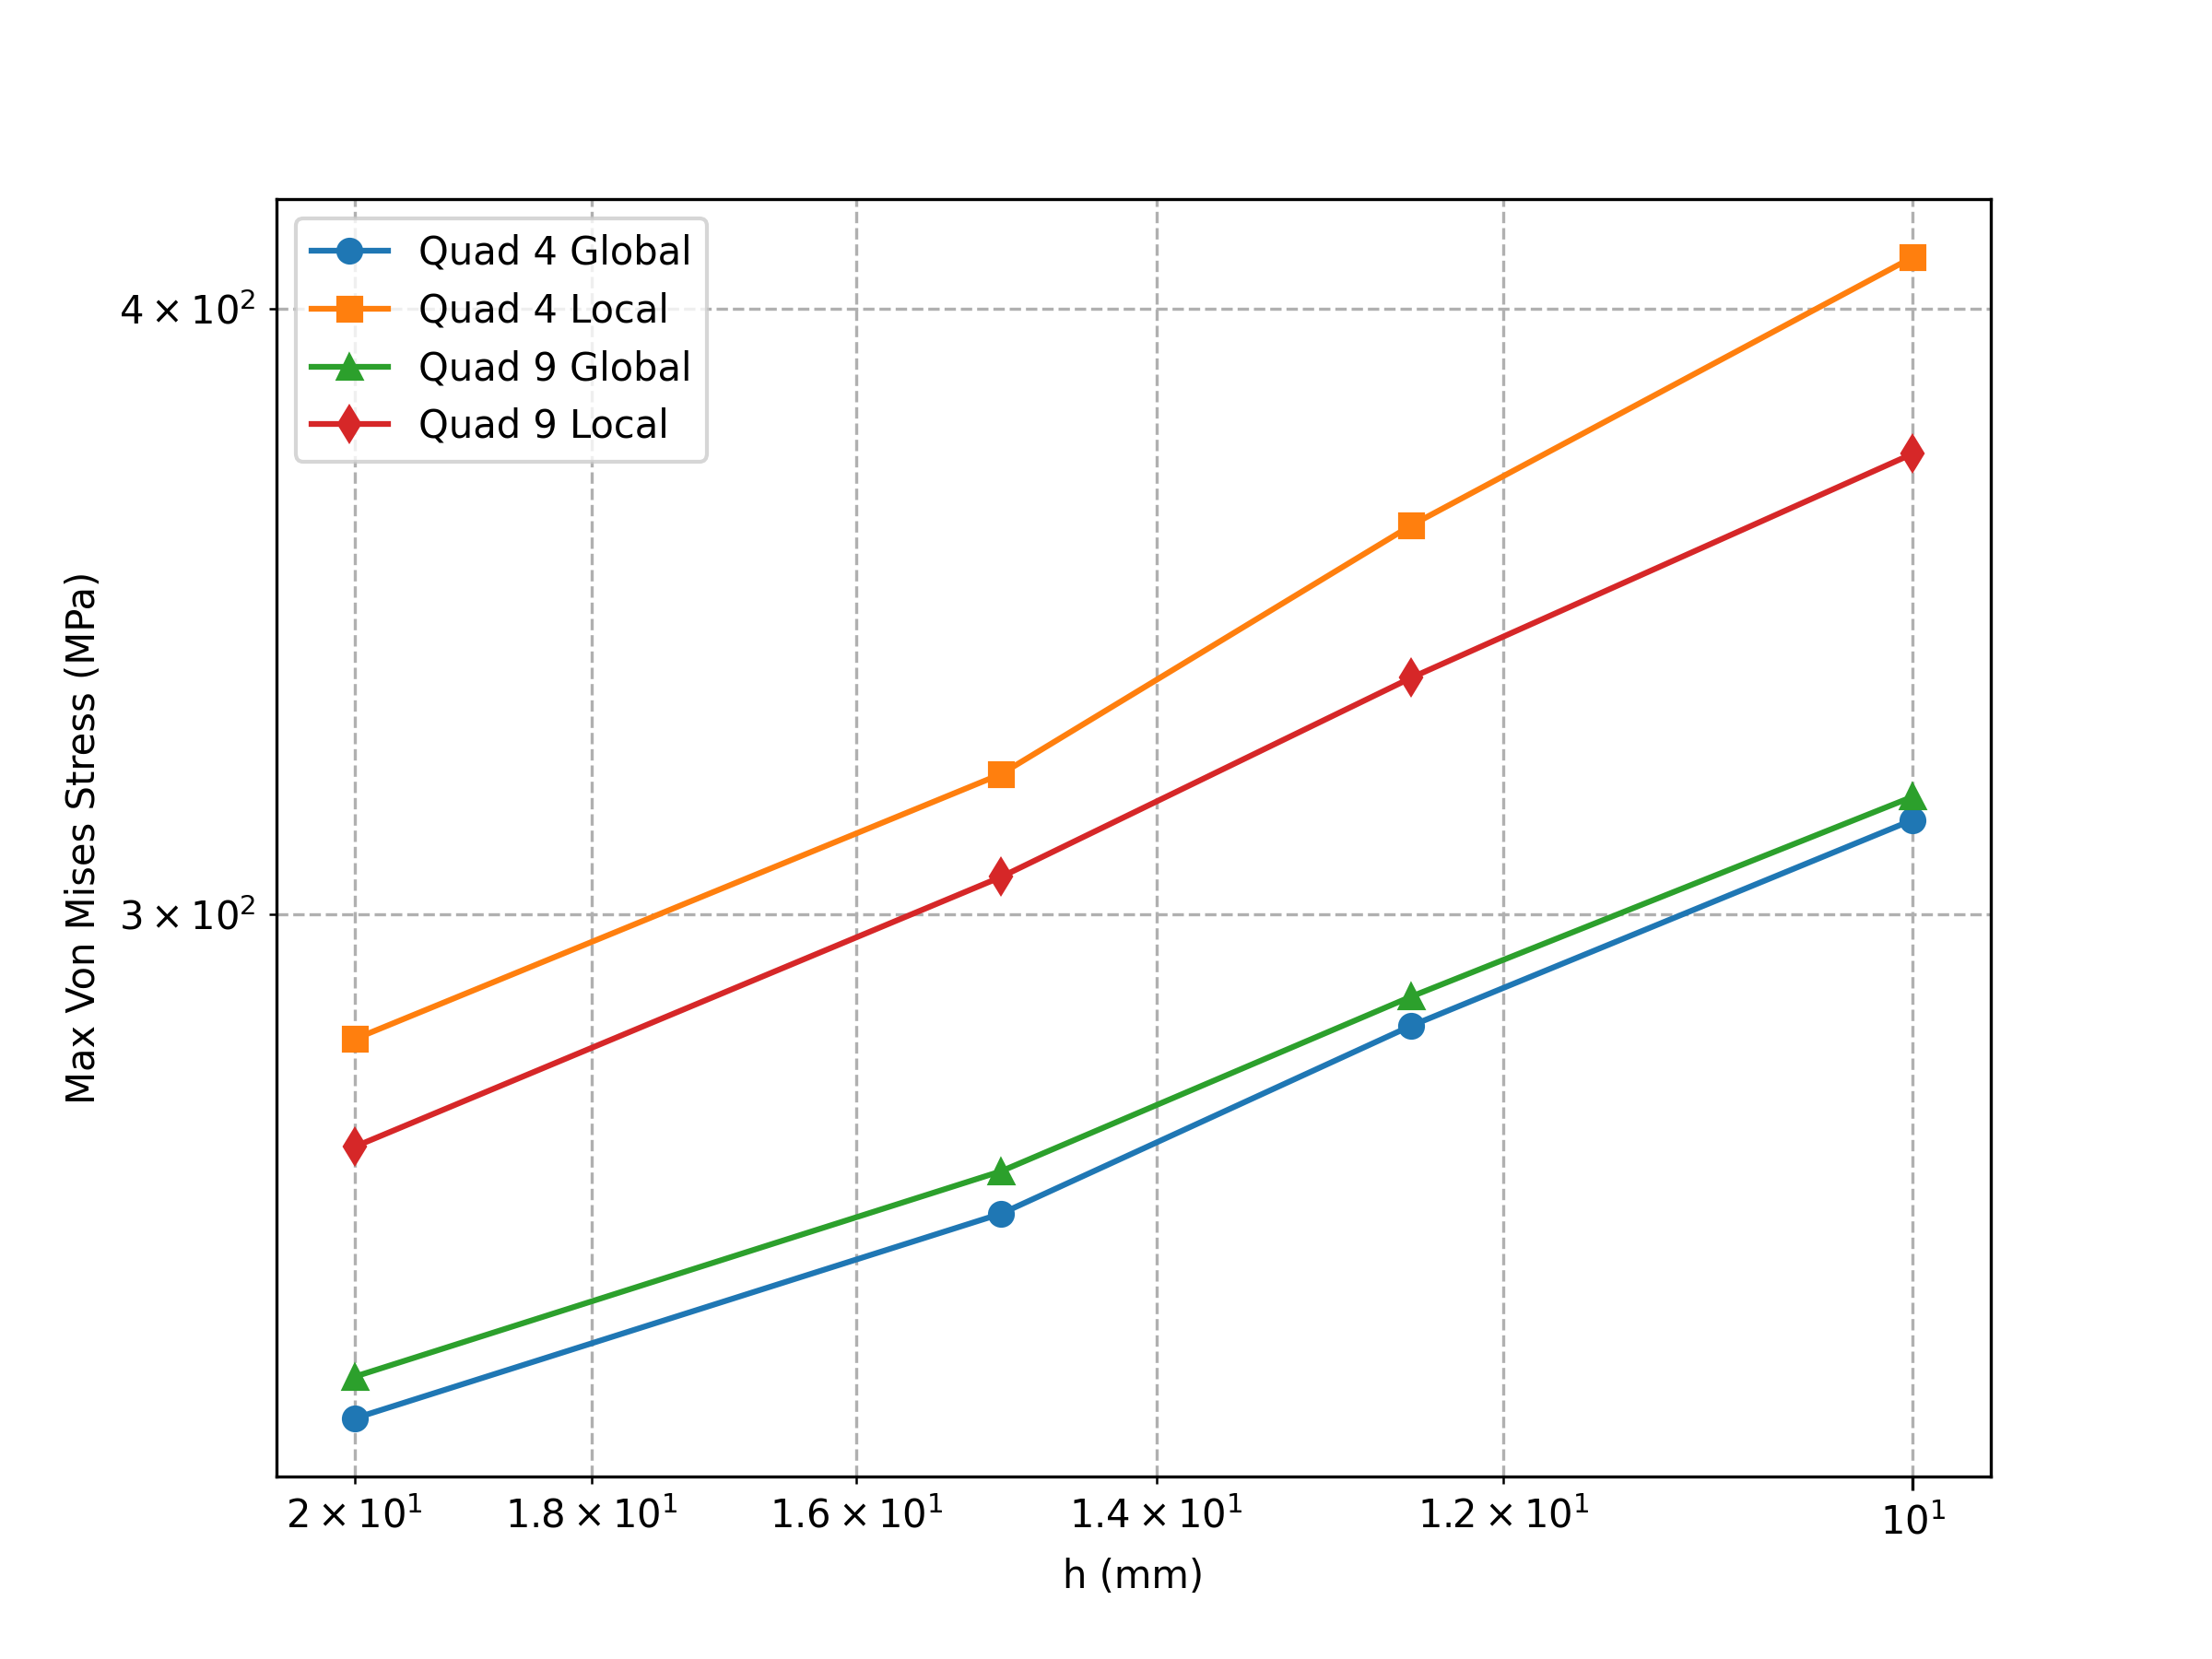
\includegraphics[width=0.5\textwidth]{GRAFICOS/convergencia.png}
    \caption{Convergence of the maximum principal stress with decreasing characteristic mesh size}
    \label{fig:convergence}
\end{figure}

Because of the maximum limit of $h=2mm$, when simulating smaller mesh sizes, the processing time increases exponentially, for that reason the curves are not significally decreasing to a convergance. Adding to the analysis, we can observe that Quad4 elements converge faster when refining the mesh locally, while Quad9 has similar behaviour in both cases.

\section{Part d) - Essay}

This assignment offered valuable lessons in the fundamentals of finite element method (FEM) modeling, specifically focusing on mesh refinement techniques and their influence on stress analysis around critical regions.

One of the primary insights was the significance of mesh refinement in accurately capturing stress concentrations. Uniformly refining the mesh throughout the model increases accuracy but at a high computational cost. Conversely, targeted local refinement, especially near geometric discontinuities, achieves comparable precision more efficiently by increasing element density only where necessary. This highlights the importance of balancing computational resources with accuracy requirements.

Through systematic analysis, it was evident that the maximum principal stress is highly sensitive to mesh density near the stress concentration. As mesh size decreases, the stress predictions converge, confirming the necessity of adequate mesh resolution in critical zones for reliable results.

Local geometric modifications, such as material removal or shape optimization near stress risers, demonstrated the profound effect design changes can have on redistributing stresses. By mitigating sharp gradients, these modifications reduce peak stresses, enhancing the structural safety and durability of the component. This emphasizes the iterative relationship between simulation and design optimization.

The assignment also shed light on practical FEM challenges, including the complexity of mesh generation, ensuring mesh compatibility (especially with structured meshes like transfinite meshing), and selecting appropriate element types. Employing higher-order elements (Quad9) and parametrized mesh control strategies proved essential in improving solution accuracy without excessive computational expense.

In reflection, the experience underscored the critical role of informed mesh refinement and design iteration in FEM. Successful modeling requires not only technical skills in software and numerical methods but also engineering judgment to focus resources where they matter most. This holistic approach ensures simulations that are both efficient and trustworthy, enabling better-informed engineering decisions.